In this chapter, we present results on the finite-volume spectrum of $\Sigma$ baryons in several $I=1$, $S=-1$ symmetry sectors, namely $G_{1g}$, $G_{1u}$, $H_u$, $H_g$, $G_{2g}$, and $G_{2u}$. We have constructed correlator matrices from large bases of single- and two-hadron operators, which allows us to more accurately determine the spectrum than in previous works. We compare our results to experimentally observed $\Sigma$ resonances, and compare to a previous work using a smaller lattice, heavier pion, and no two-hadron operators.

The $\Sigma$ baryons are unstable resonances. However, lattice QCD Monte Carlo results are obtained in finite volume.  In finite volume, only the energies of the finite-volume stationary states can be determined.  To deduce the spectrum of resonances from the finite-volume energies would require a technique similar to that employed by L\"uscher~\cite{Luscher:1990ck} but extended beyond two-particle thresholds.  Such a technique does not yet exist and would be prohibitively difficult to carry out.  Our goal here is much more humble.  We wish mainly to identify the finite-volume states produced primarily by three-quark single baryon operators.  The energies of such states are expected to fall near the resonance energies of the $\Sigma$ baryons which are predominantly three-quark excitations.  The narrower the resonance, the closer our estimates should be.  In other words, our results should be viewed as a qualitative study of the resonance spectrum.  Note that resonances which are primarily ``molecular'' in nature cannot be determined in this way.  Futhermore, our use of an unphysical light quark mass to make the calculations practical will cause further deviations from experiment.

All past studies~\cite{Edwards:2012fx, Bulava:2009jb, Bulava:2010yg, Edwards:2011jj} suffer from these same flaws.  However, all past studies have only used single baryon operators.  This study is the first to also use meson-baryon operators, significantly improving the spectrum determination.
\section{Ensemble}
Ensemble details are identical to those described in Sec.~\ref{sec:ensemble}.
\section{$G_{1g}$ Spectrum}
The isotriplet, $S=-1$, $G_{1g}$ symmetry channel is parity-positive and contains spins $\frac{1}{2}$, $\frac{7}{2}$, $\frac{9}{2}$, and beyond. In this channel, we expect to see several experimentally observed states including the physical $\Sigma$, the $\Sigma(1660)$, and the $\Sigma(2030)$, which have spins $\frac{1}{2}$, $\frac{1}{2}$, and $\frac{7}{2}$, respectively. In addition to these single-hadron states, we expect to see many multi-hadron states. Reliably extracting finite-volume single-hadron states that correspond to resonances in infinite-volume requires the use of multi-hadron operators, since we expect the finite-volume counterpart to a resonance to have some overlap onto its decay products. While it would be ideal to compute many-hadron correlators, computing correlators for states with greater than two hadrons is prohibitively expensive, so we limit ourselves to using operators which are designed to create at most two hadrons.

In general, we start with a large basis of operators, and \emph{prune} out those which are either too noisy or not sufficiently linearly independent. For the single-hadron operators, we started with a large basis 16 operators, and pruned our set down to just 7. For the two-hadron operators, we started with a basis of 25 operators, and pruned our set down to just 21. The final basis of single- and two-hadron operators used to extract the spectrum in this channel is given in Table~\ref{table:g1g_ops}. Just as in Sec.~\ref{sec:a0}, we make use of variationally improved single-hadron operators. That is, we first diagonalize in the subspace of single-hadron operators to form linear combinations which overlap more independently onto the single-hadron states of interest, in order to aid in level identification. We found that a normalization time, metric time, and diagonalization time of $\tau_N=3$, $\tau_0=4$, and $\tau_d=7$ ensured that the rotated correlator matrix remained sufficiently diagonal. It is important to note that while $\eta\Sigma$ two-hadron operators are included, there is no corresponding $\phi\Sigma$ operator, so we expect to miss a two-hadron state. This will be the case in every channel in this chapter.

\begin{table}[H]
    \centering
    \begin{tabular}{l|l}
        \textbf{Single-Hadron Operators} & \textbf{Two-Hadron Operators} \\
        \hline
        $\Sigma_{G_{1g}}^{DDI0}$ & $\pi(0)_{A_{1u}^-}^{SS0}\Lambda(0)_{G_{1u}}^{SS2}$\\
        $\Sigma_{G_{1g}}^{DDI22}$ & $\pi(0)_{A_{1u}^-}^{SS0}\Lambda(0)_{G_{1u}}^{SS3}$\\
        $\Sigma_{G_{1g}}^{DDL55}$ & $\pi(1)_{A_2^-}^{SS1}\Lambda(1)_{G_1}^{SS1}$\\
        $\Sigma_{G_{1g}}^{SS2}$ & $\pi(2)_{A_2^-}^{SS0}\Lambda(2)_{G}^{SS0}$\\
        $\Sigma_{G_{1g}}^{SS3}$ & $\pi(3)_{A_2^-}^{SS0}\Lambda(3)_{G}^{SS0}$\\
        $\Sigma_{G_{1g}}^{TDT65}$ & $\pi(1)_{A_2^-}^{SS0}\Sigma(1)_{G_1}^{SS0}$\\
        $\Sigma_{G_{1g}}^{TDT72}$ & $\pi(1)_{A_2^-}^{SS1}\Sigma(1)_{G_1}^{SS0}$\\
        & $\pi(1)_{A_2^-}^{SS1}\Sigma(1)_{G_1}^{SS2}$\\
        & $\pi(2)_{A_2^-}^{SS0}\Sigma(2)_{G}^{SS1}$\\
        & $\pi(3)_{A_2^-}^{SS0}\Sigma(3)_{G}^{SS4}$\\
        & $\overline K(1)_{A_1}^{SS2}N(1)_{G_1}^{SS0}$\\
        & $\overline K(1)_{A_2}^{SS0}N(1)_{G_1}^{SS0}$\\
        & $\overline K(1)_{A_2}^{SS1}N(1)_{G_1}^{SS0}$\\
        & $\overline K(1)_{E}^{SS2}N(1)_{G_1}^{SS0}$\\
        & $\overline K(4)_{A_2}^{SS1}N(4)_{G_1}^{SS0}$\\
        & $\overline K(2)_{A_2}^{SS0}N(2)_{G}^{SS0}$\\
        & $\overline K(2)_{A_2}^{SS1}N(2)_{G}^{SS0}$\\
        & $\overline K(3)_{A_2}^{SS0}N(3)_{G}^{SS0}$\\
        & $\overline K(1)_{A_2}^{SS1}\Delta(1)_{G_1}^{SS0}$\\
        & $K(1)_{A_2}^{SS1}\Xi(1)_{G_1}^{SS0}$\\
        & $\eta(1)_{A_2^+}^{SS1}\Sigma(1)_{G_1}^{SS0}$
    \end{tabular}
    \caption{Operators used in the isotriplet $S=-1$ $G_{1g}$ symmetry sector.}\label{table:g1g_ops}
\end{table}
The spectrum obtained in terms of the kaon mass (obtained from the fit given in Ch.~\ref{ch:tetraquarks}) is shown in Fig.~\ref{fig:g1g_spectrum}. Correlator fits are shown in Fig.~\ref{fig:g1g_fits}, and fit details are given in Table~\ref{table:g1g_fits}. A qualitative attempt at level identification is made by determining, for each operator, which level overlaps maximally with the state created by that operator. Additionally, we are interested in operators which have significant but non-maximal overlaps onto a given state, which can inform us about mixing. Mixing is important since we expect a resonance to have overlap onto not only states created by single-hadron operators, but also states corresponding to potential decay products. A comparison of the experimentally observed resonances in this channel to the low-lying single-hadron-dominated states we obtain from the lattice is shown in Fig.~\ref{fig:g1g_exp}. Because we do not expect to reliably extract the masses of the highest few levels, we do not include the highest two single-hadron-dominated states in our comparison to experiment, and their energy determinations should be viewed as being much less reliable. When comparing results to experiment, we use the nucleon mass (obtained from the fit shown in Fig.~\ref{fig:nucleon_fit}) as a reference, since it is more sensitive than the kaon mass to the unphysically heavy pion. However, we are able to determine the kaon mass with better precision, so we use it as a reference in our full spectrum plots, e.g. Fig~\ref{fig:g1g_spectrum}. Our findings seem to agree qualitatively with previous lattice results by Edwards et al.\ in Ref.~\cite{Edwards:2012fx}, shown in Fig.~\ref{fig:edwards}, produced using a $16^3$ lattice with a pion mass of $m_\pi \approx 391$ MeV and no two-hadron operators. In Ref.~\cite{Edwards:2012fx}, they found one low-lying state, corresponding to the physical $\Sigma$, and four higher nearly-degenerate states with two less well determined levels just above the four levels. We find the same pattern: one low-lying level, with four higher well-determined nearly-degenerate levels, and two more states nearby but not well determined.

In comparing our results to experiment, we see qualitative agreement in energy: A well-determined ground state corresponding to the physical $\Sigma$ and several states above it near in energy to the $\Sigma(1660)$ and the $\Sigma(2030)$. Our results are certainly affected by our unphysically heavy pion and the fact that we are comparing infinite-volume resonances to their finite-volume stationary-state counterpart, however, so we should not expect rigorous agreement. Additionally, as will be the case in many of the other channels in this chapter, we do not find agreement between the number of single-hadron-dominated states on the lattice and the number of resonances seen in experiment in the same energy range. This should not come as a surprise, however. The problem of ``missing resonances''~\cite{Koniuk:1979vw} has long been an issue; the number of baryon resonances predicted by quark models has long disagreed with the number seen in experiment. In Ref.~\cite{Koniuk:1979vw}, Koniuk and Isgur attempt to explain this by claiming that over half of all predicted resonances are too inelastic to be easily seen.

\begin{figure}[H]
    \centering
    \hspace*{-0.5in}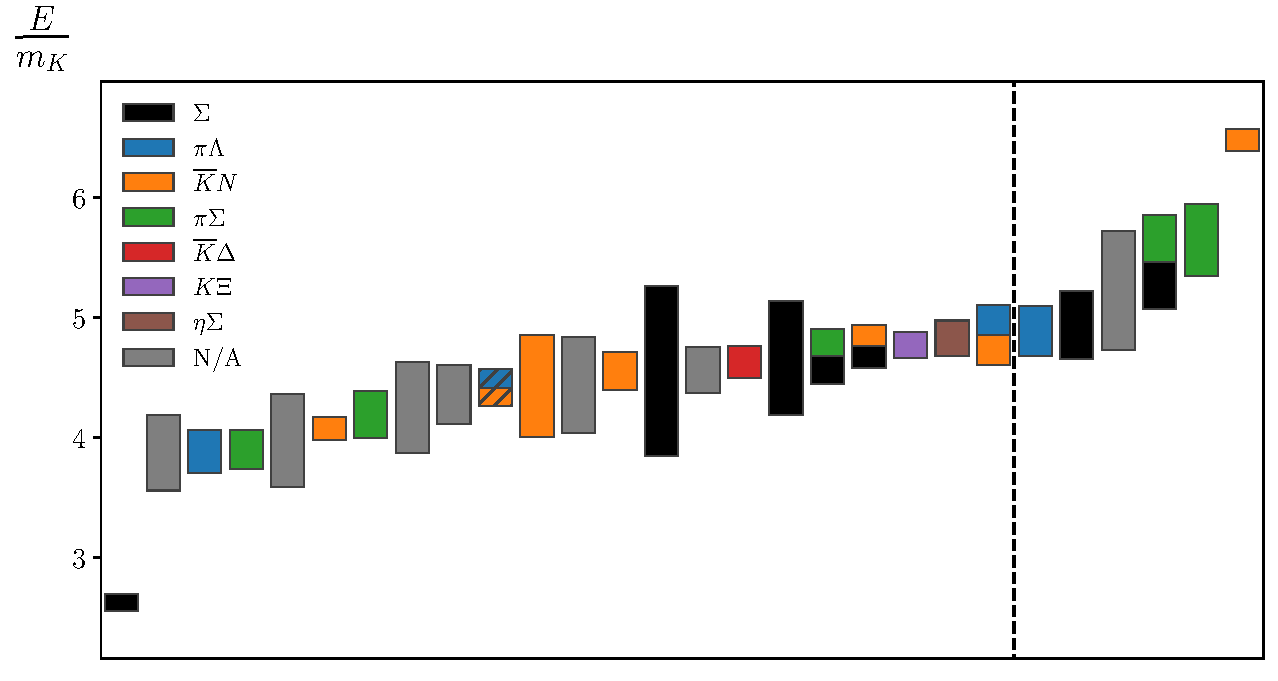
\includegraphics[width=\textwidth]{figures/sigmas/g1g/staircase_mk.pdf}
    \caption[The spectrum for the isotriplet $S=-1$ $G_{1g}$ channel, obtained by fitting the energies and overlap factors of the diagonalized correlator matrix.]{The spectrum for the isotriplet $S=-1$ $G_{1g}$ channel, obtained by fitting the energies and overlap factors of the diagonalized correlator matrix. A qualitative attempt at level identification is made by determining, for each operator, which level overlaps maximally with the state created by that operator. If a level does not overlap maximally with any operator's state, we denote its flavor content as ``N/A''. Because we expect a single-hadron resonance to have significant overlap with potential decay products, we also use hatching to denote any level which has an overlap of $\geq 70\%$ of the maximum overlap with a single-hadron operator. The vertical dashed line indicates the point beyond which our energy extractions are too high to be reliable.}\label{fig:g1g_spectrum}
\end{figure}

\begin{figure}[H]
    \centering
    \hspace*{-1cm}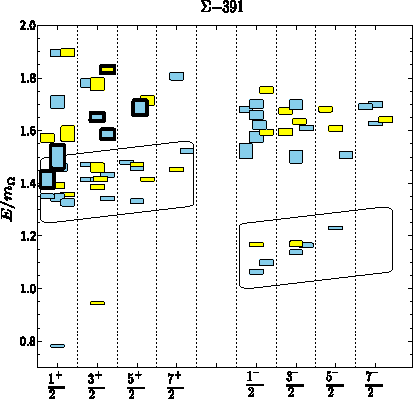
\includegraphics[width=0.8\textwidth]{figures/edwards.pdf}
    \caption[Observed single-hadron states on a $16^3$ lattice with a pion mass of $m_\pi \approx 391$, sorted by $J^P$ quantum numbers, from Ref.~\cite{Edwards:2012fx}.]{Observed single-hadron states on a $16^3$ lattice with a pion mass of $m_\pi \approx 391$, sorted by $J^P$ quantum numbers, from Ref.~\cite{Edwards:2012fx}. Colors indicate SU(3)-flavor irrep, which we do not identify.}\label{fig:edwards}
\end{figure}

\begin{figure}[H]
    \centering
    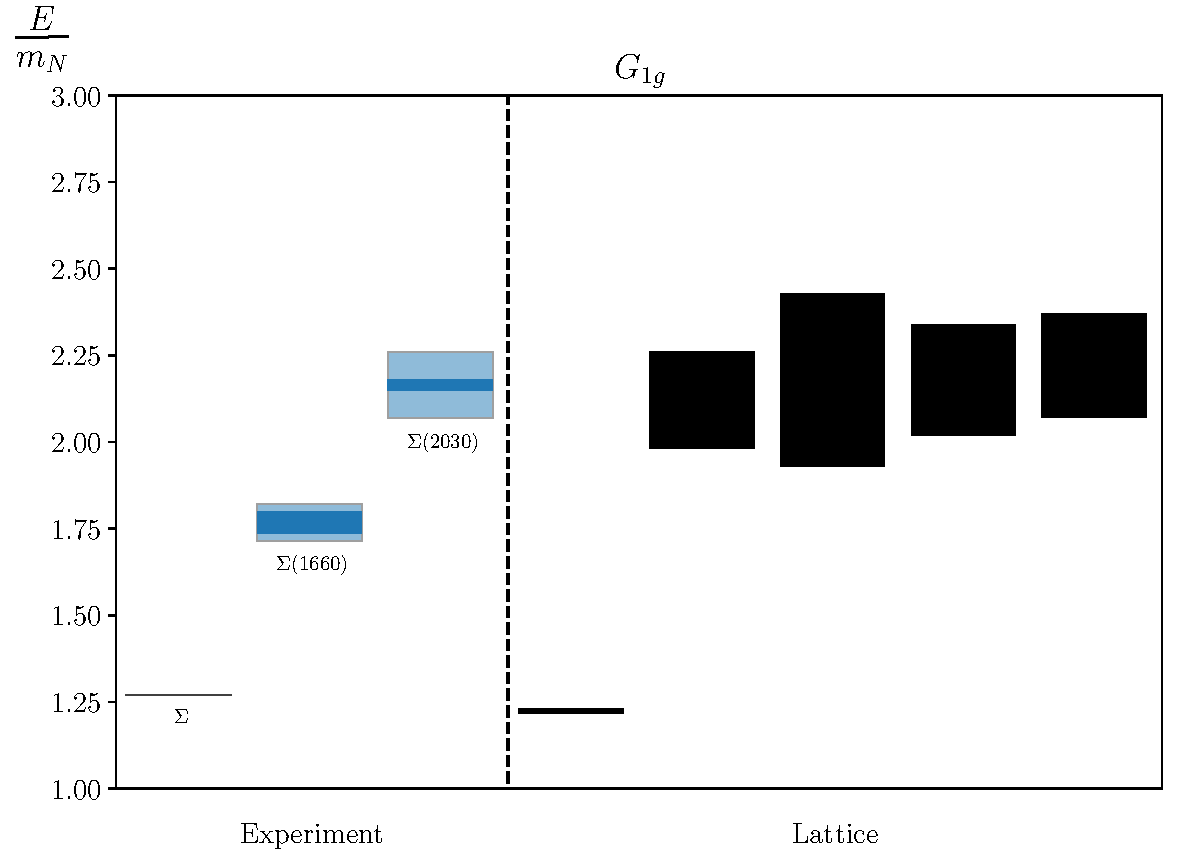
\includegraphics[width=0.8\textwidth]{figures/sigmas/g1g/expvslat.pdf}
    \caption[Experimentally observed resonances compared with the finite-volume single-hadron-dominated stationary states we obtain from the lattice in $G_{1g}$, in terms of the nucleon mass.]{Experimentally observed resonances compared with the finite-volume single-hadron-dominated stationary states we obtain from the lattice, in terms of the nucleon mass. For the experimental states, dark bands indicate experimental uncertainty and light bands indicate decay widths.}\label{fig:g1g_exp}
\end{figure}

\begin{figure}[H]
    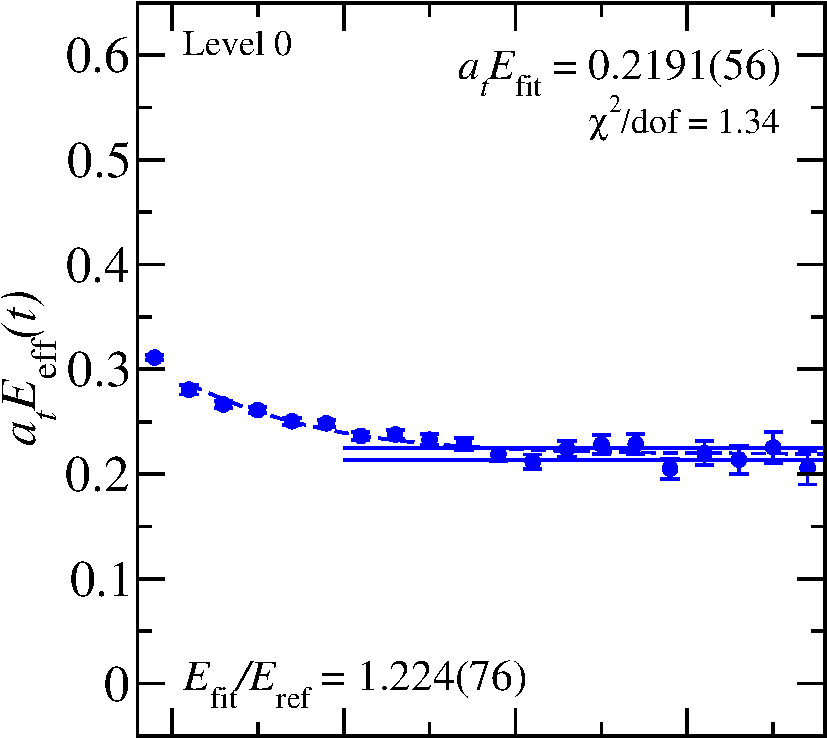
\includegraphics[width=0.215\textwidth]{figures/sigmas/g1g/fits/fit_0.pdf}
    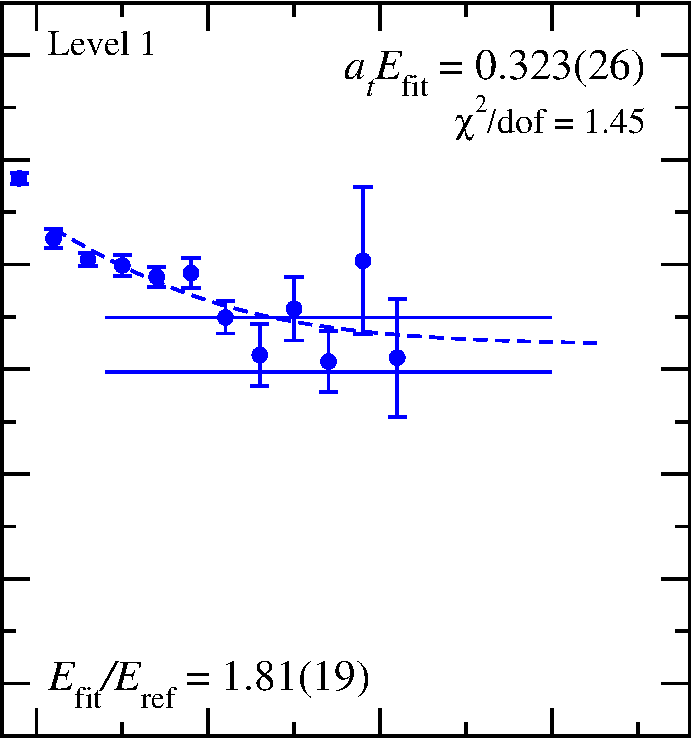
\includegraphics[width=0.18\textwidth]{figures/sigmas/g1g/fits/fit_7.pdf}
    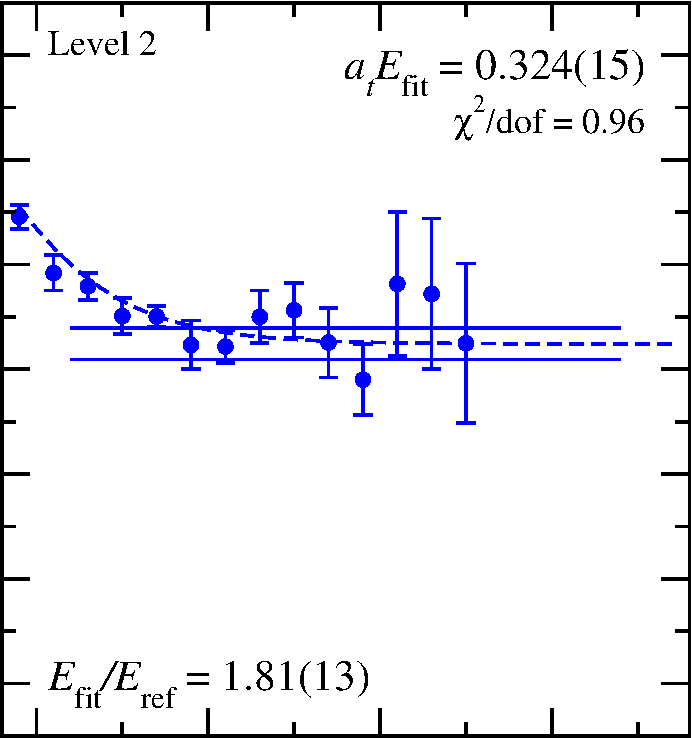
\includegraphics[width=0.18\textwidth]{figures/sigmas/g1g/fits/fit_3.pdf}
    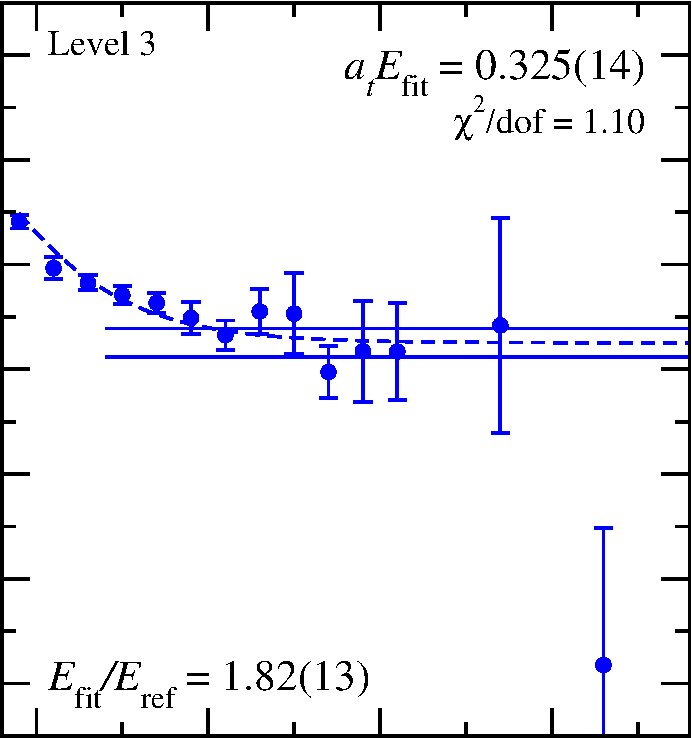
\includegraphics[width=0.18\textwidth]{figures/sigmas/g1g/fits/fit_4.pdf}
    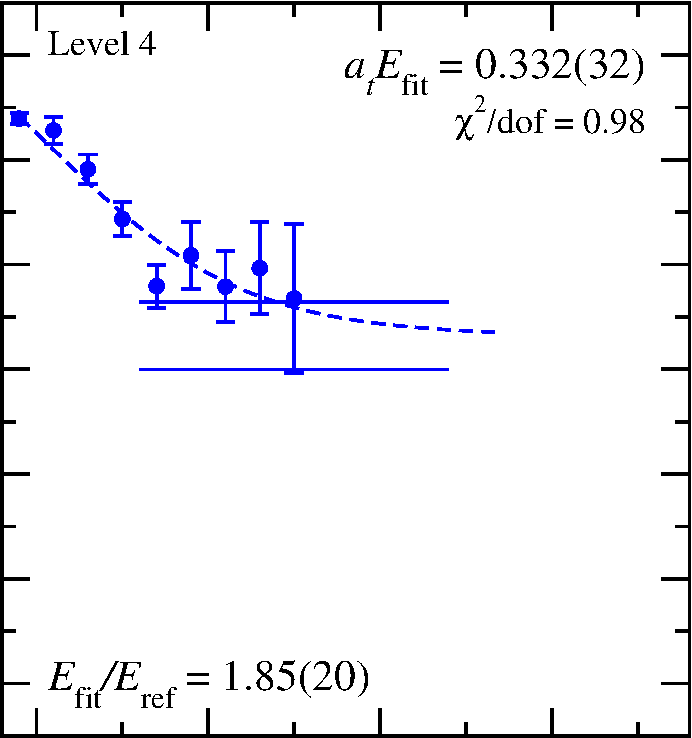
\includegraphics[width=0.18\textwidth]{figures/sigmas/g1g/fits/fit_21.pdf}\\
    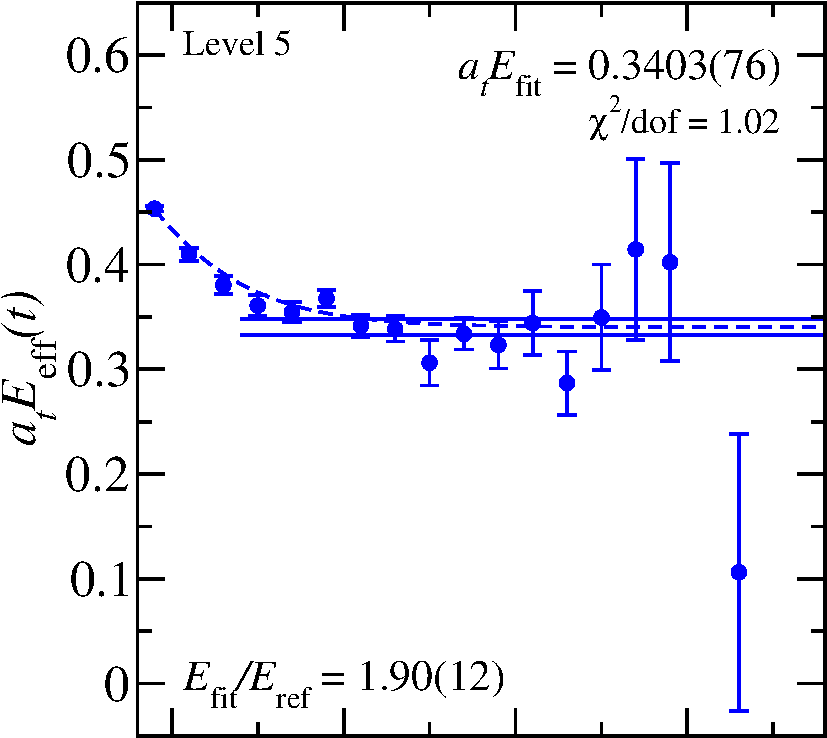
\includegraphics[width=0.215\textwidth]{figures/sigmas/g1g/fits/fit_5.pdf}
    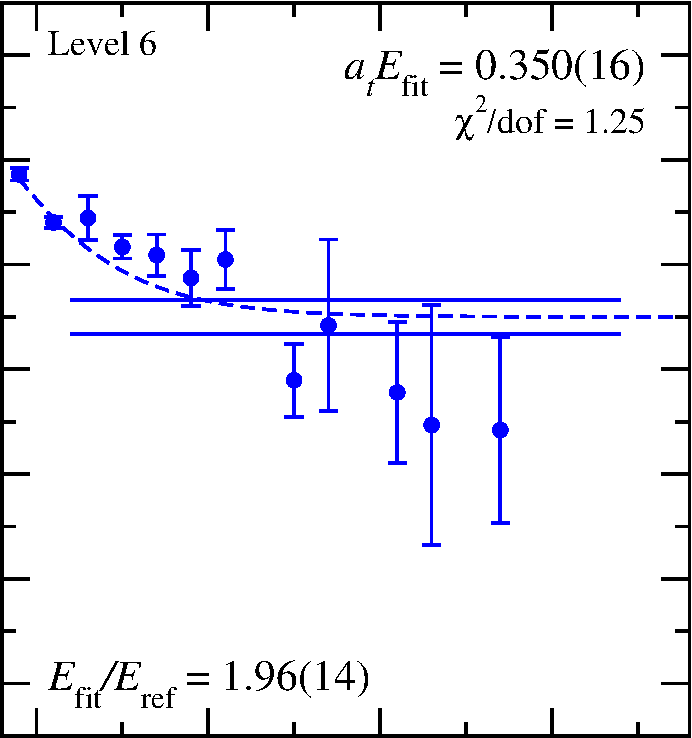
\includegraphics[width=0.18\textwidth]{figures/sigmas/g1g/fits/fit_9.pdf}
    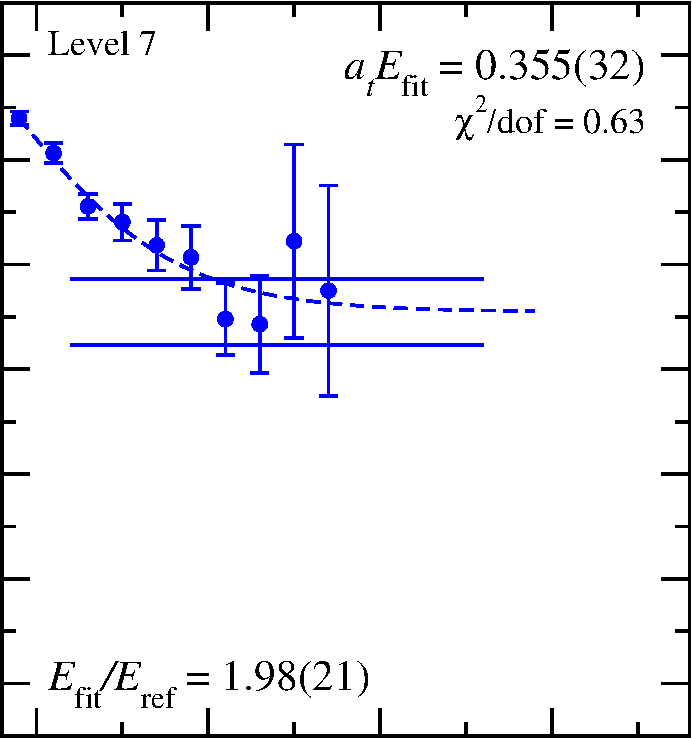
\includegraphics[width=0.18\textwidth]{figures/sigmas/g1g/fits/fit_19.pdf}
    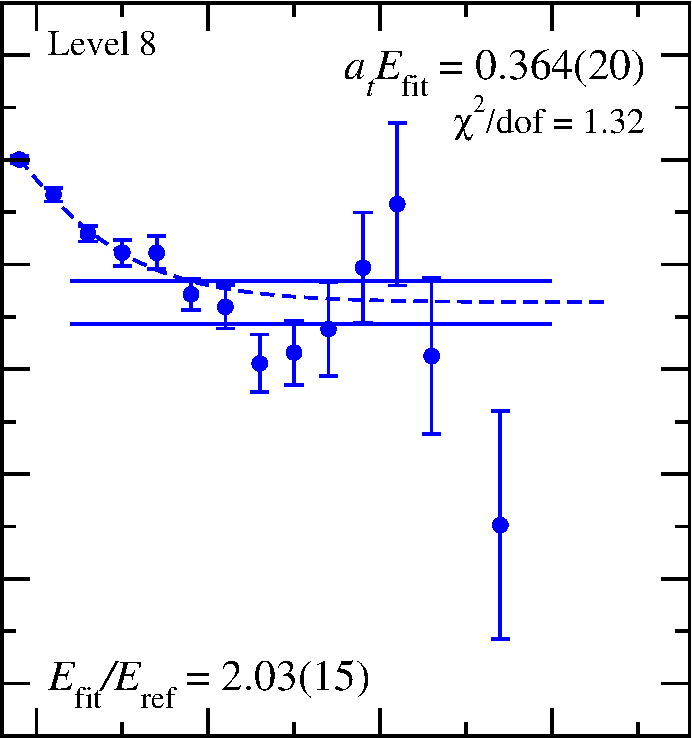
\includegraphics[width=0.18\textwidth]{figures/sigmas/g1g/fits/fit_14.pdf}
    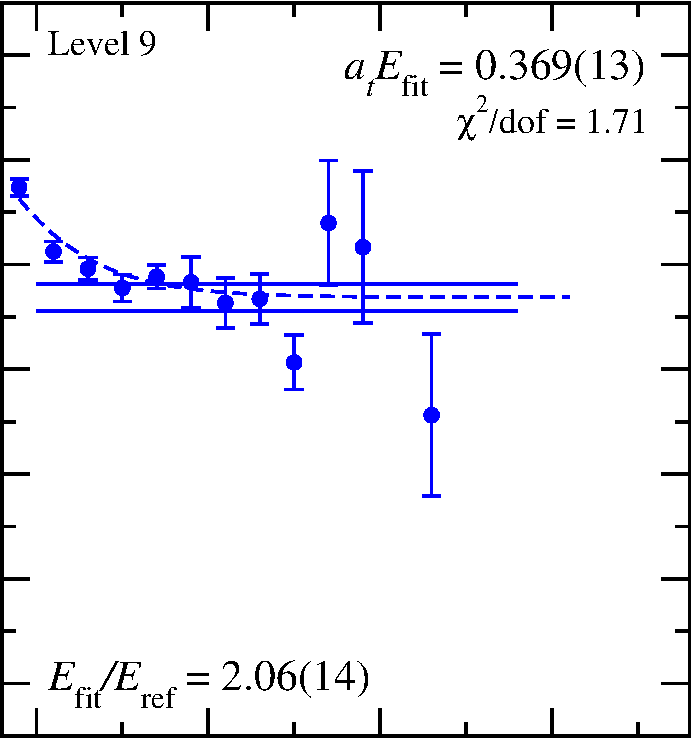
\includegraphics[width=0.18\textwidth]{figures/sigmas/g1g/fits/fit_6.pdf}\\
    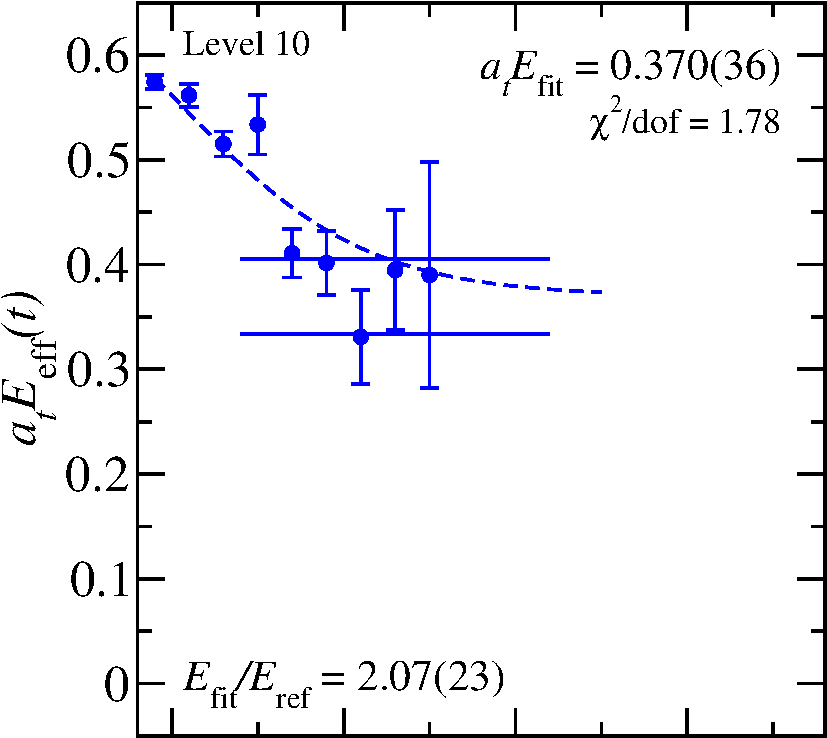
\includegraphics[width=0.215\textwidth]{figures/sigmas/g1g/fits/fit_23.pdf}
    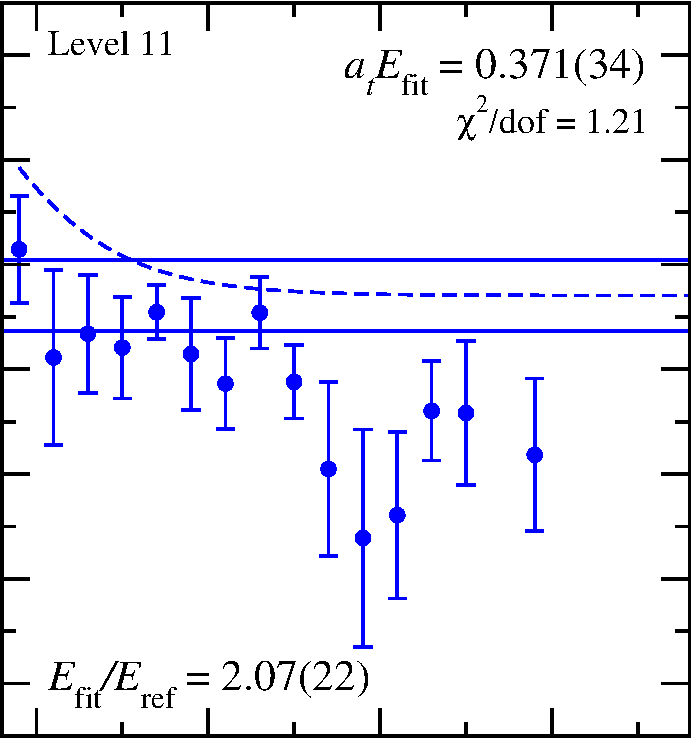
\includegraphics[width=0.18\textwidth]{figures/sigmas/g1g/fits/fit_1.pdf}
    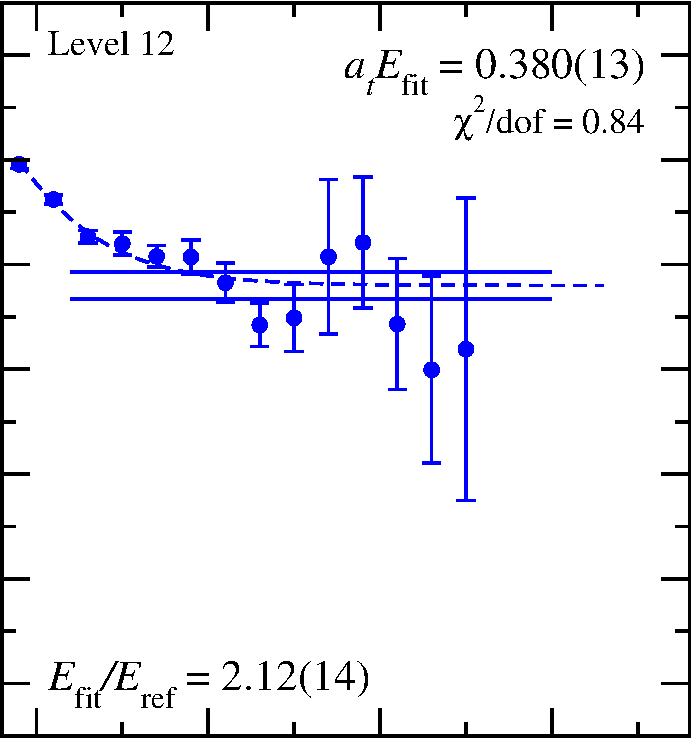
\includegraphics[width=0.18\textwidth]{figures/sigmas/g1g/fits/fit_13.pdf}
    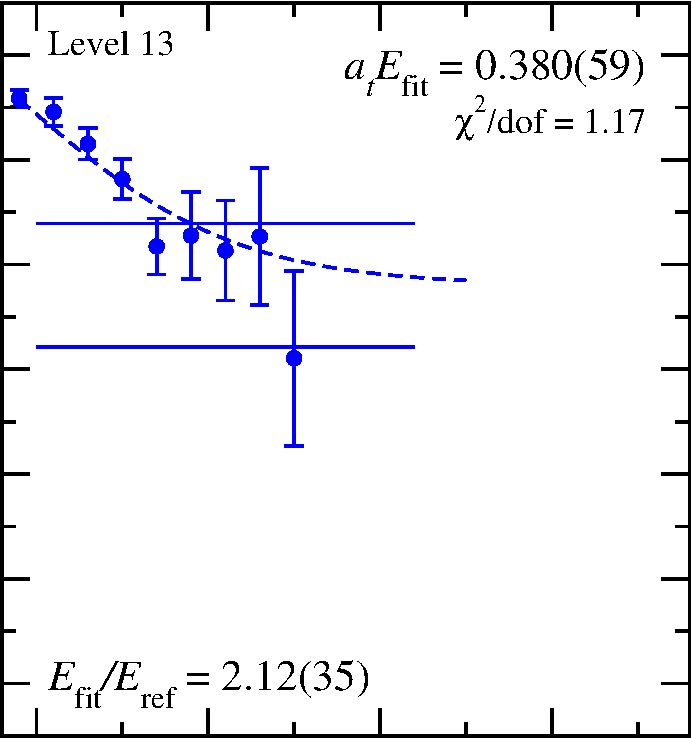
\includegraphics[width=0.18\textwidth]{figures/sigmas/g1g/fits/fit_22.pdf}
    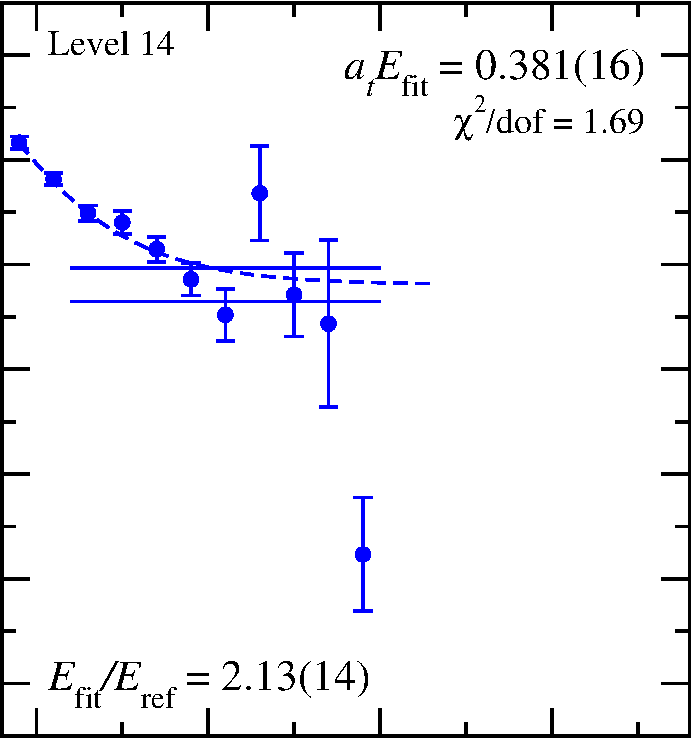
\includegraphics[width=0.18\textwidth]{figures/sigmas/g1g/fits/fit_16.pdf}\\
    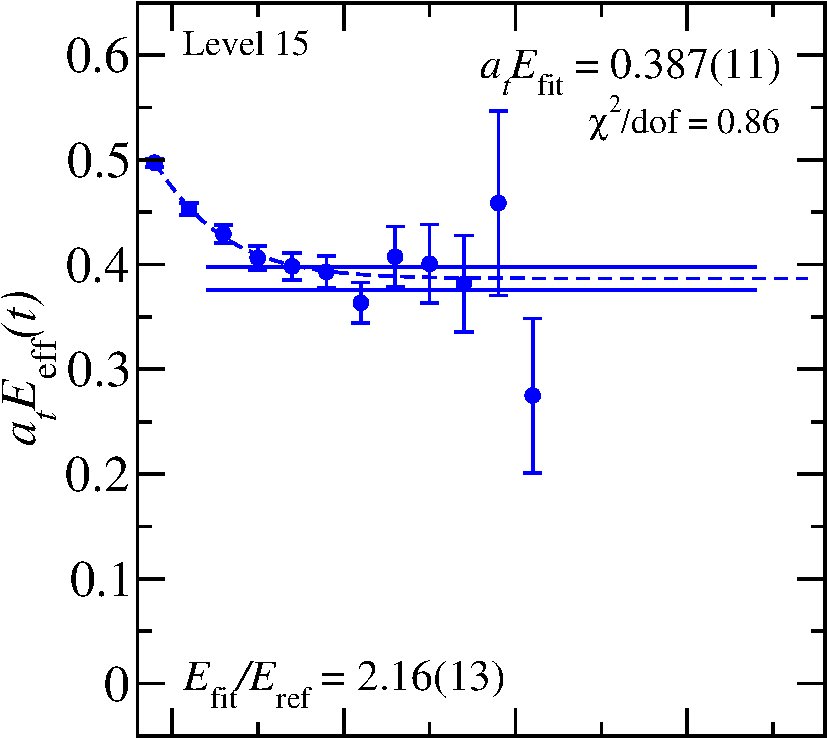
\includegraphics[width=0.215\textwidth]{figures/sigmas/g1g/fits/fit_11.pdf}
    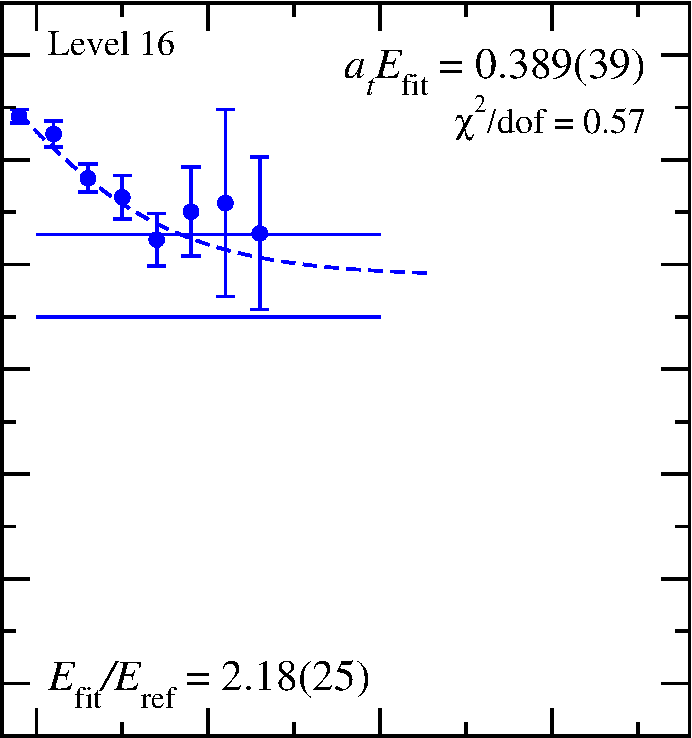
\includegraphics[width=0.18\textwidth]{figures/sigmas/g1g/fits/fit_20.pdf}
    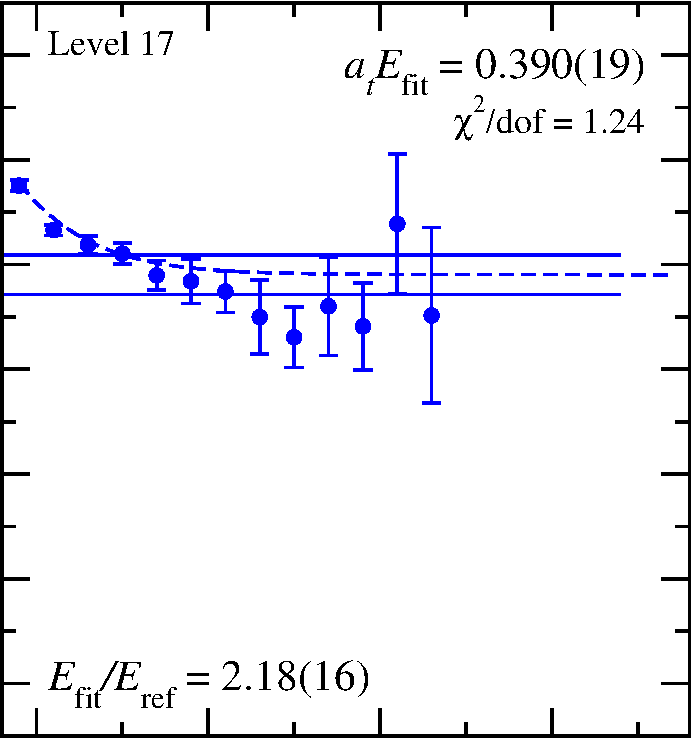
\includegraphics[width=0.18\textwidth]{figures/sigmas/g1g/fits/fit_8.pdf}
    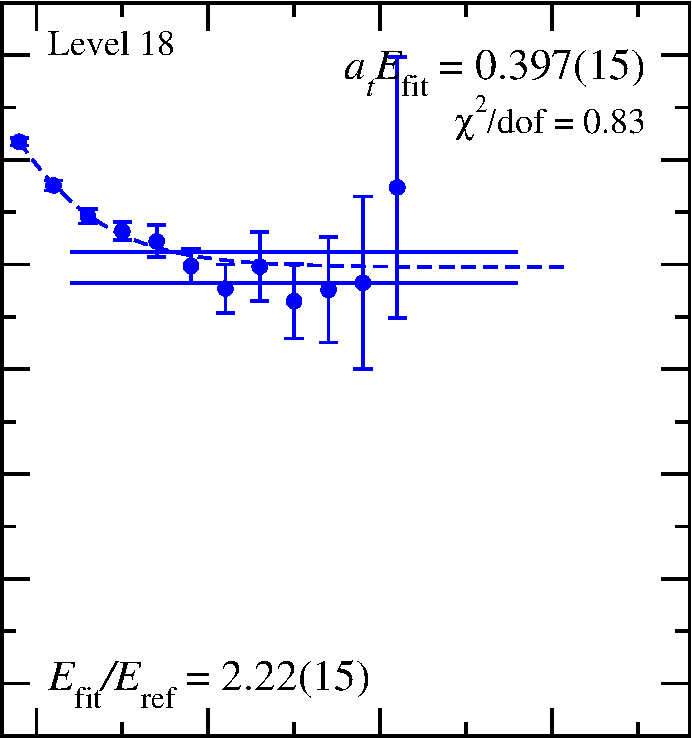
\includegraphics[width=0.18\textwidth]{figures/sigmas/g1g/fits/fit_15.pdf}
    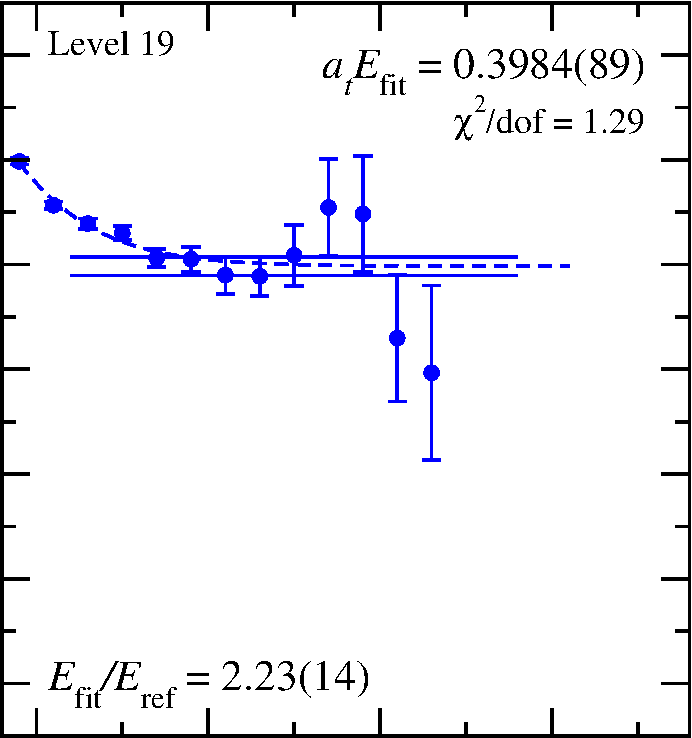
\includegraphics[width=0.18\textwidth]{figures/sigmas/g1g/fits/fit_12.pdf}\\
    \raisebox{0.35cm}{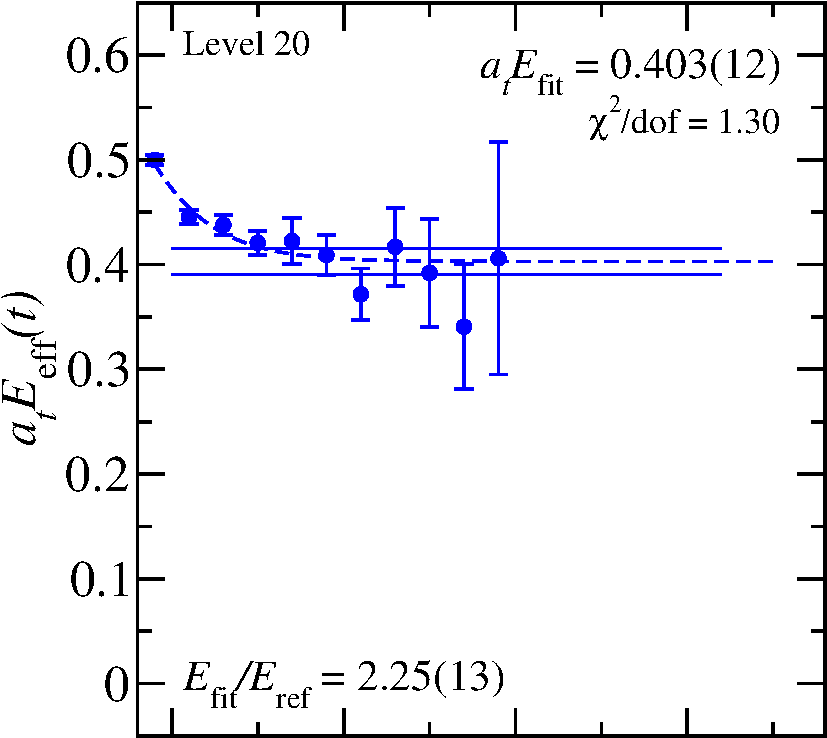
\includegraphics[width=0.215\textwidth]{figures/sigmas/g1g/fits/fit_10.pdf}}
    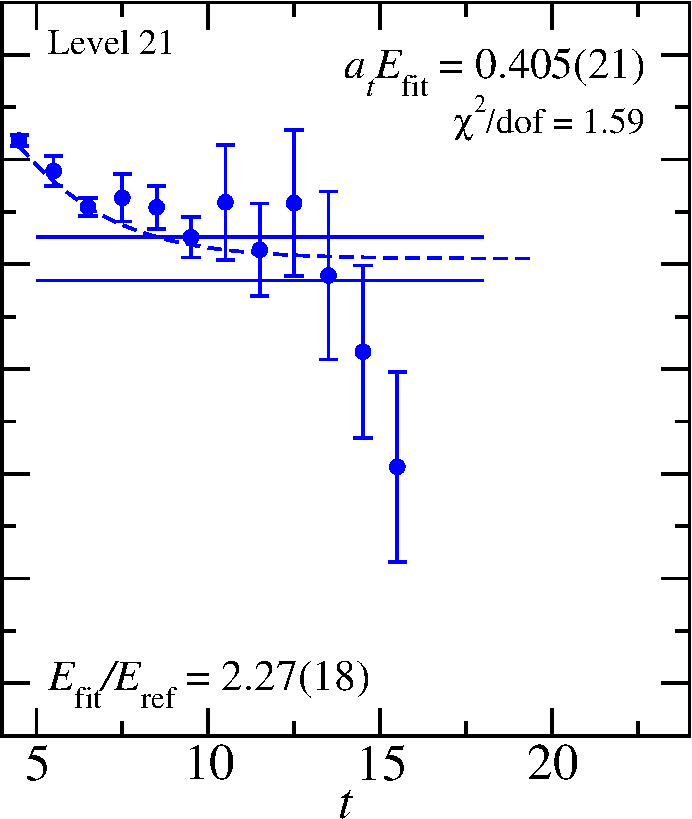
\includegraphics[width=0.18\textwidth]{figures/sigmas/g1g/fits/fit_17.pdf}
    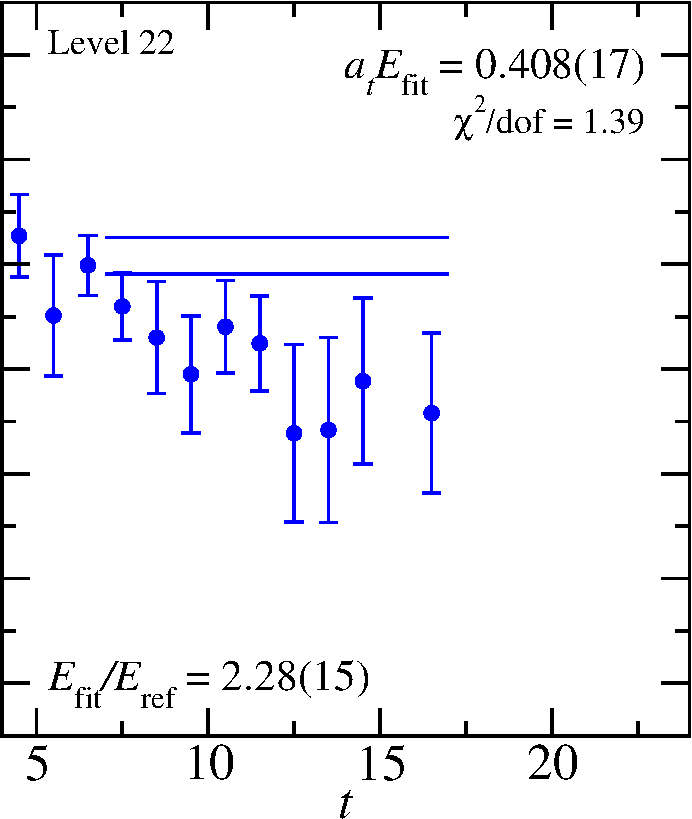
\includegraphics[width=0.18\textwidth]{figures/sigmas/g1g/fits/fit_2.pdf}
    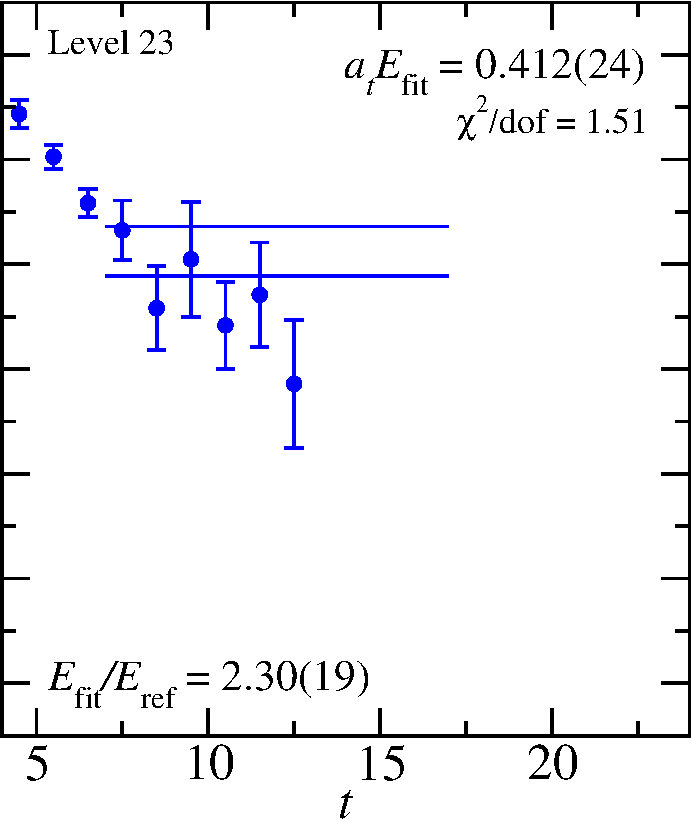
\includegraphics[width=0.18\textwidth]{figures/sigmas/g1g/fits/fit_18.pdf}
    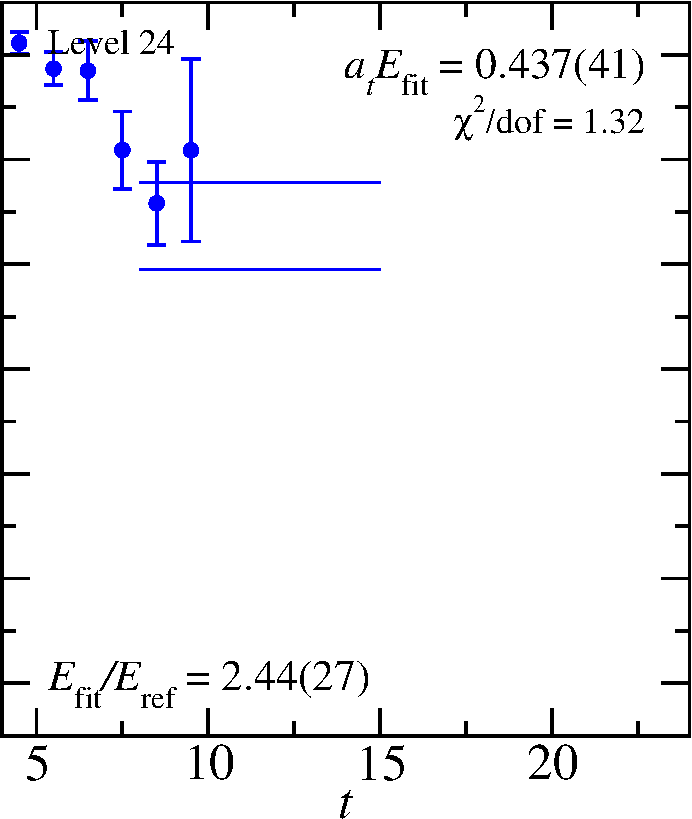
\includegraphics[width=0.18\textwidth]{figures/sigmas/g1g/fits/fit_25.pdf}\\[-0.35cm]
    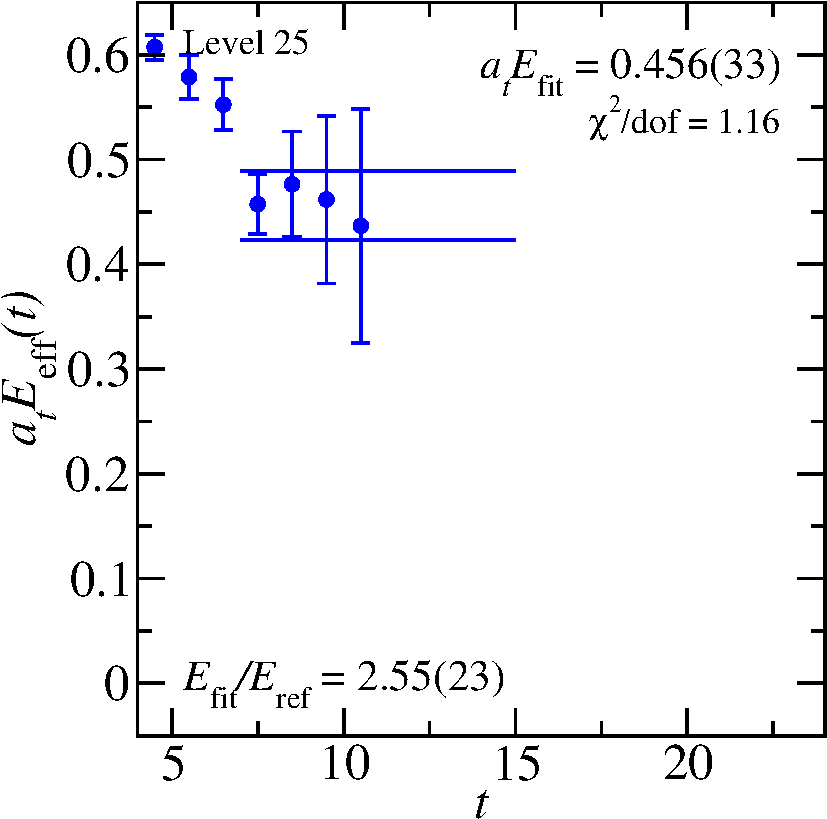
\includegraphics[width=0.215\textwidth]{figures/sigmas/g1g/fits/fit_24.pdf}
    \caption[Effective energies for the rotated $28\times 28$ correlator matrix in the isotriplet $S=-1$ $G_{1g}$ symmetry channel.]{Effective energies for the rotated $28\times 28$ correlator matrix in the isotriplet $S=-1$ $G_{1g}$ symmetry channel. Effective energy curves calculated from correlator fits are overlaid, and fit results are shown. The nucleon mass is used as a reference.}\label{fig:g1g_fits}
\end{figure}

\begin{figure}[H]
    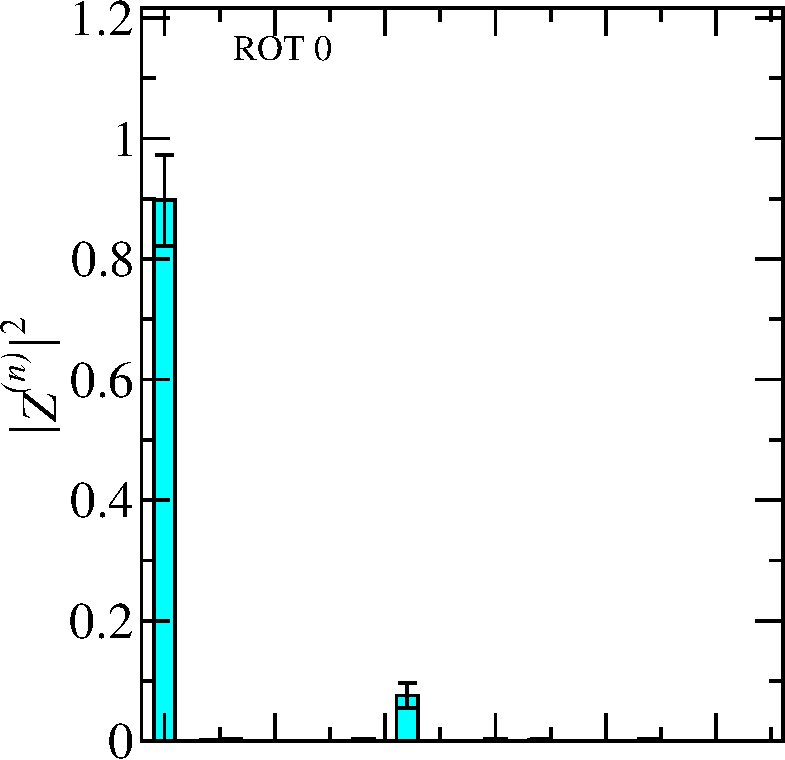
\includegraphics[width=.1975\textwidth]{figures/sigmas/g1g/zfactors/zfactor_isotriplet-S-1-P000-G1g_1-ROT-0.pdf}
    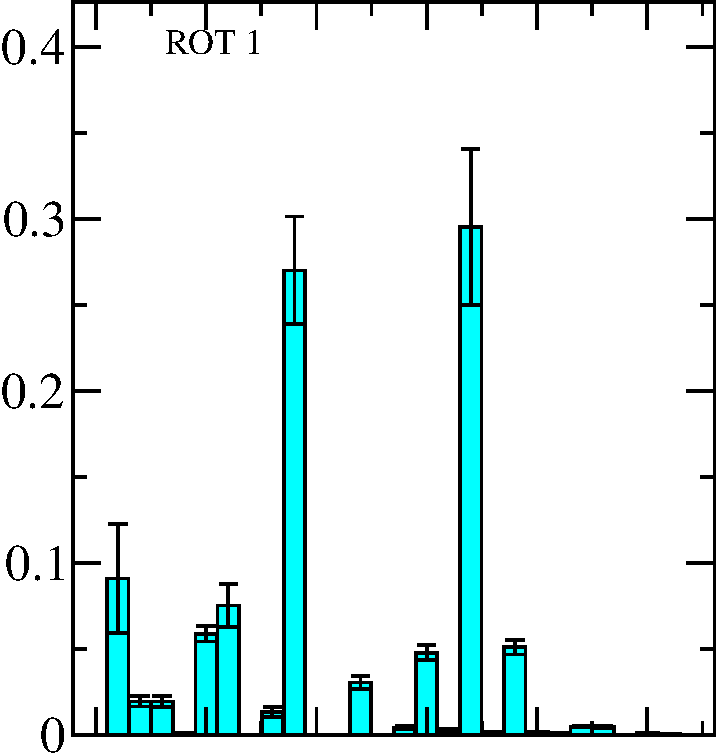
\includegraphics[width=.18\textwidth]{figures/sigmas/g1g/zfactors/zfactor_isotriplet-S-1-P000-G1g_1-ROT-1.pdf}
    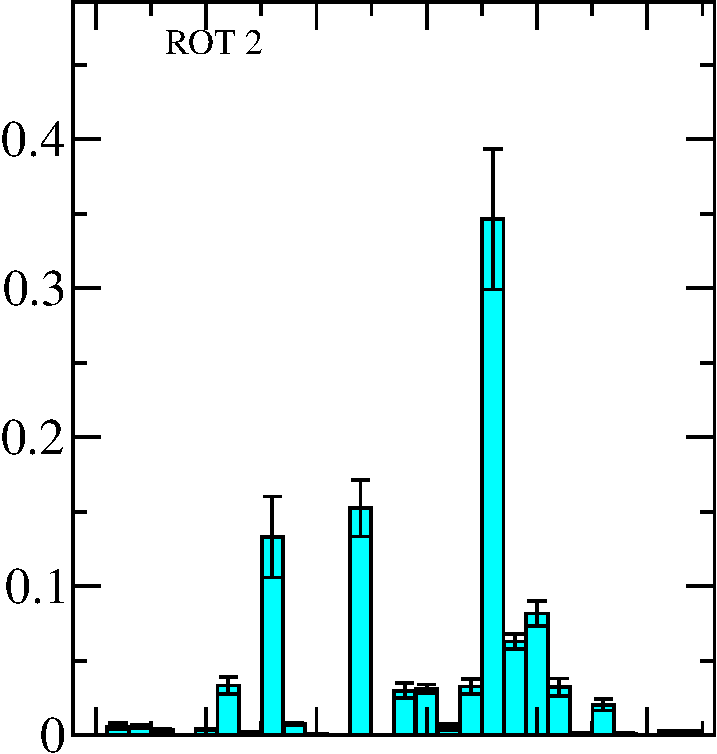
\includegraphics[width=.18\textwidth]{figures/sigmas/g1g/zfactors/zfactor_isotriplet-S-1-P000-G1g_1-ROT-2.pdf}
    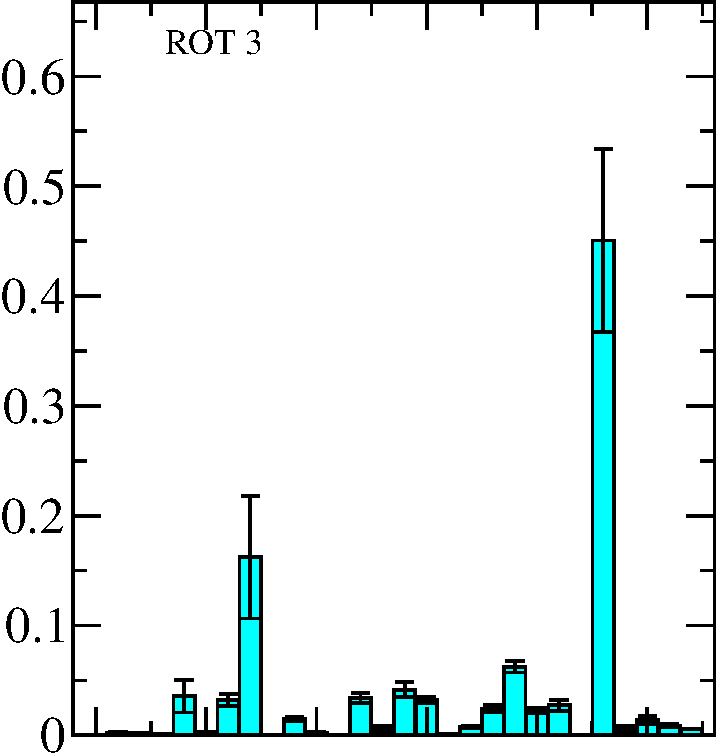
\includegraphics[width=.18\textwidth]{figures/sigmas/g1g/zfactors/zfactor_isotriplet-S-1-P000-G1g_1-ROT-3.pdf}
    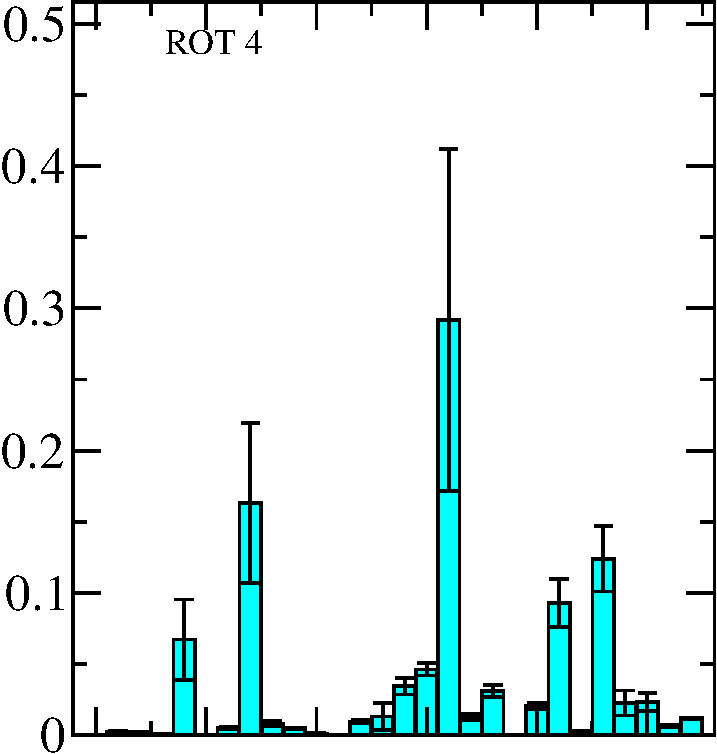
\includegraphics[width=.18\textwidth]{figures/sigmas/g1g/zfactors/zfactor_isotriplet-S-1-P000-G1g_1-ROT-4.pdf}\\
    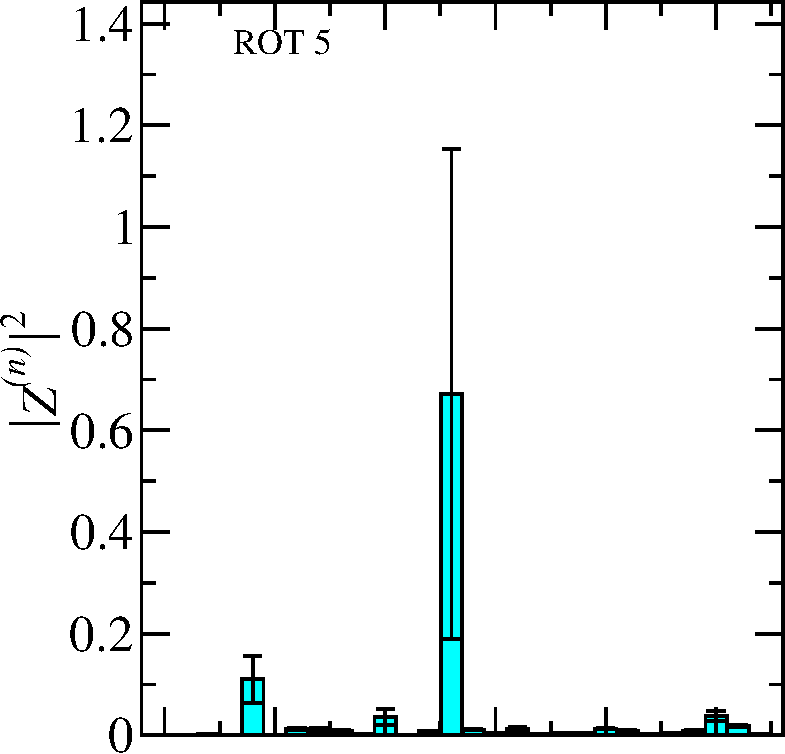
\includegraphics[width=.1975\textwidth]{figures/sigmas/g1g/zfactors/zfactor_isotriplet-S-1-P000-G1g_1-ROT-5.pdf}
    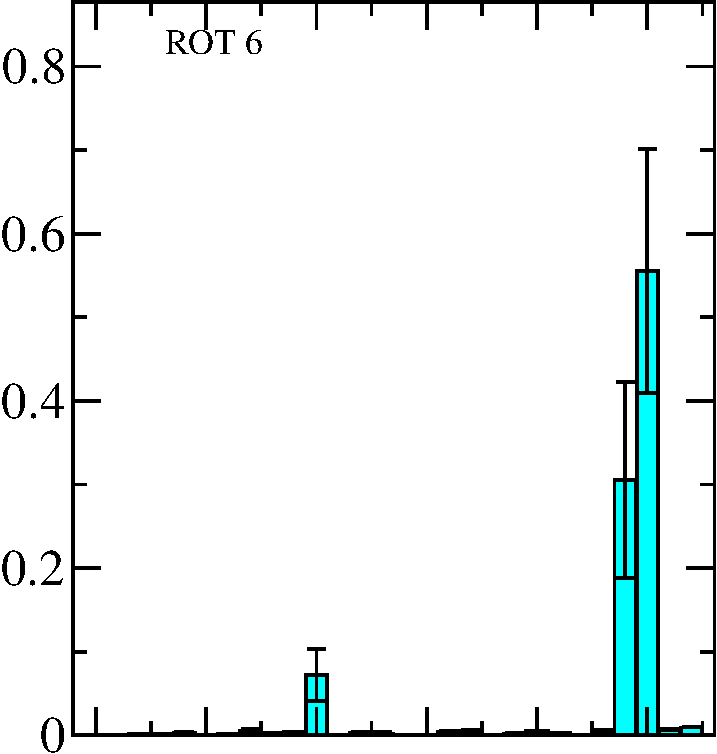
\includegraphics[width=.18\textwidth]{figures/sigmas/g1g/zfactors/zfactor_isotriplet-S-1-P000-G1g_1-ROT-6.pdf}
    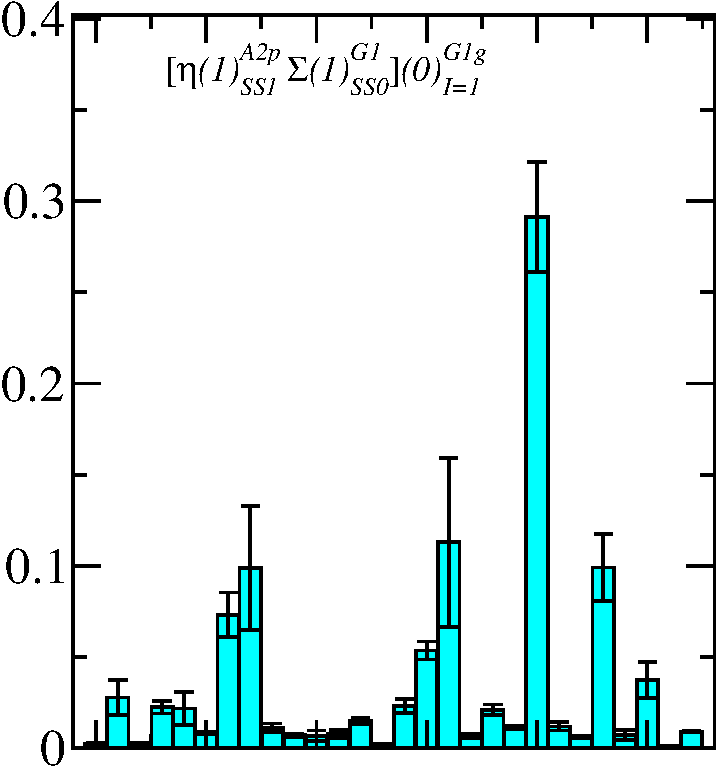
\includegraphics[width=.18\textwidth]{figures/sigmas/g1g/zfactors/zfactor_isotriplet_eta_sigma-G1g_1-P001-A2p-SS_1-P00-1-G1-SS_0.pdf}
    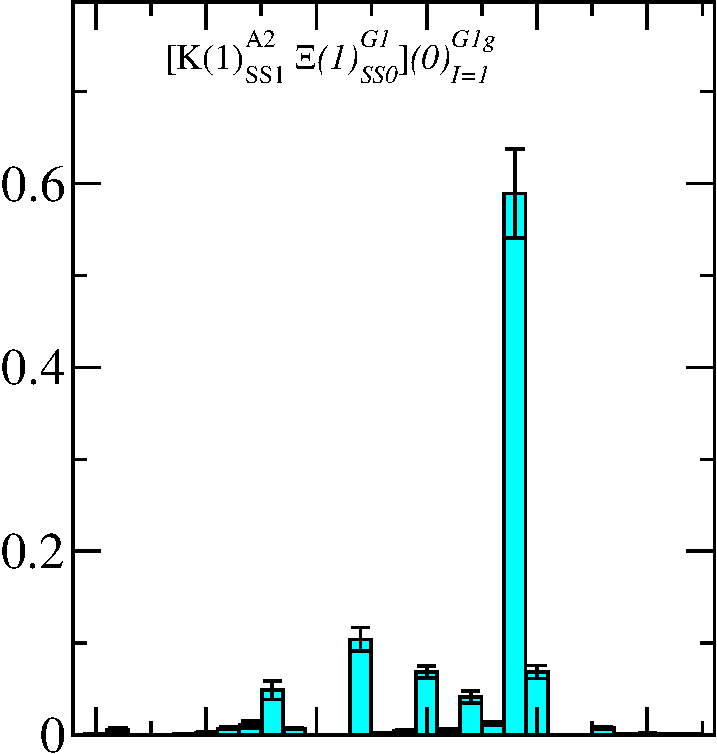
\includegraphics[width=.18\textwidth]{figures/sigmas/g1g/zfactors/zfactor_isotriplet_kaon_xi-G1g_1-P001-A2-SS_1-P00-1-G1-SS_0.pdf}
    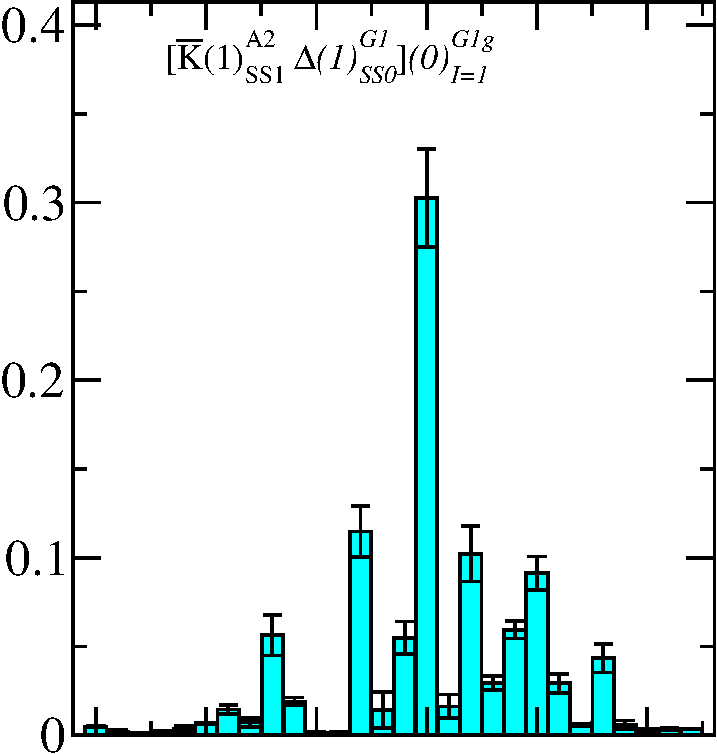
\includegraphics[width=.18\textwidth]{figures/sigmas/g1g/zfactors/zfactor_isotriplet_kbar_delta-G1g_1-P001-A2-SS_1-P00-1-G1-SS_0.pdf}\\
    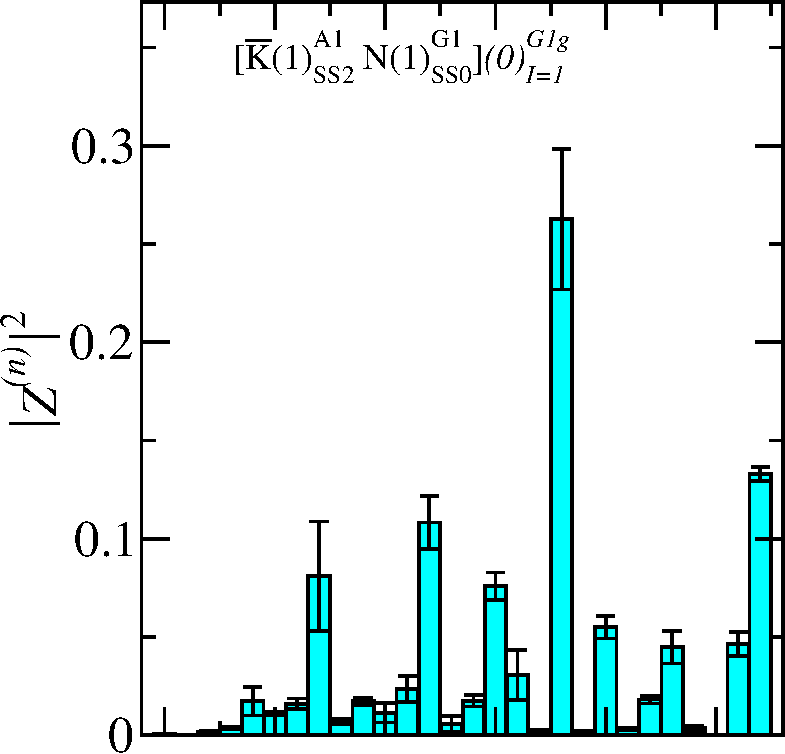
\includegraphics[width=.1975\textwidth]{figures/sigmas/g1g/zfactors/zfactor_isotriplet_kbar_nucleon-G1g_1-P001-A1-SS_2-P00-1-G1-SS_0.pdf}
    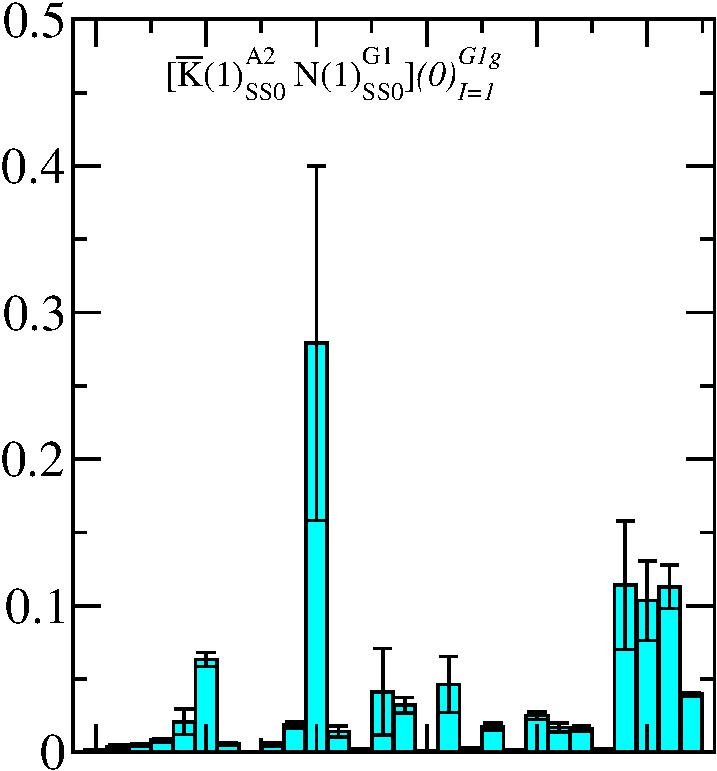
\includegraphics[width=.18\textwidth]{figures/sigmas/g1g/zfactors/zfactor_isotriplet_kbar_nucleon-G1g_1-P001-A2-SS_0-P00-1-G1-SS_0.pdf}
    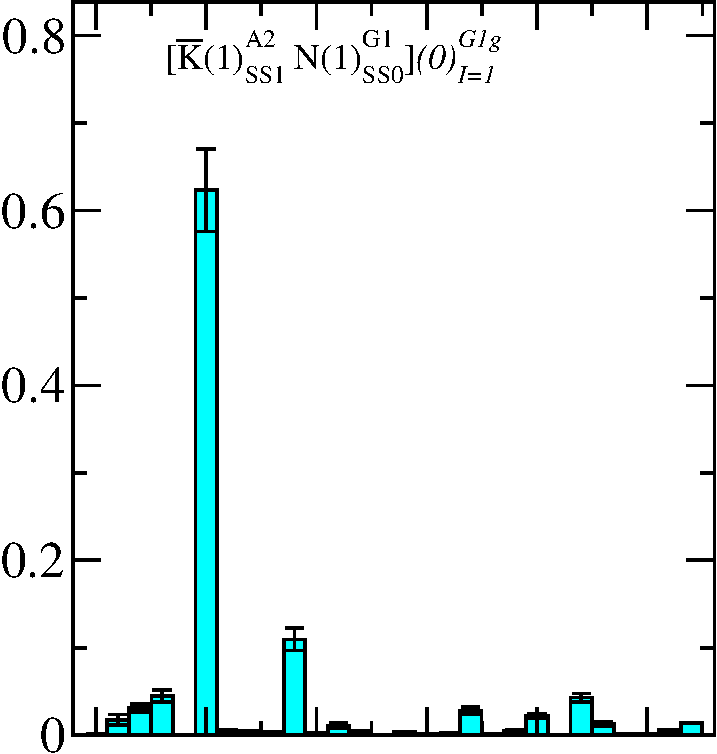
\includegraphics[width=.18\textwidth]{figures/sigmas/g1g/zfactors/zfactor_isotriplet_kbar_nucleon-G1g_1-P001-A2-SS_1-P00-1-G1-SS_0.pdf}
    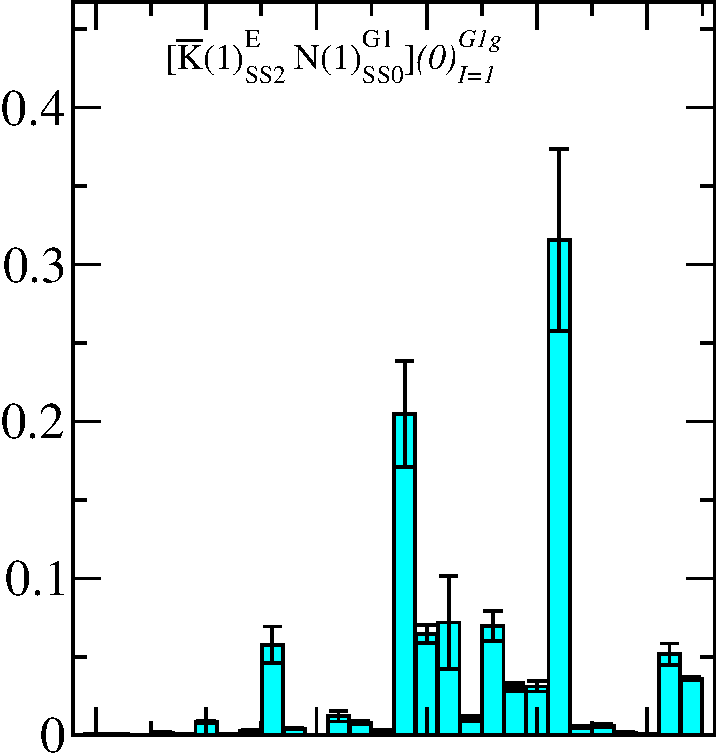
\includegraphics[width=.18\textwidth]{figures/sigmas/g1g/zfactors/zfactor_isotriplet_kbar_nucleon-G1g_1-P001-E-SS_2-P00-1-G1-SS_0.pdf}
    \hspace*{-0.1cm}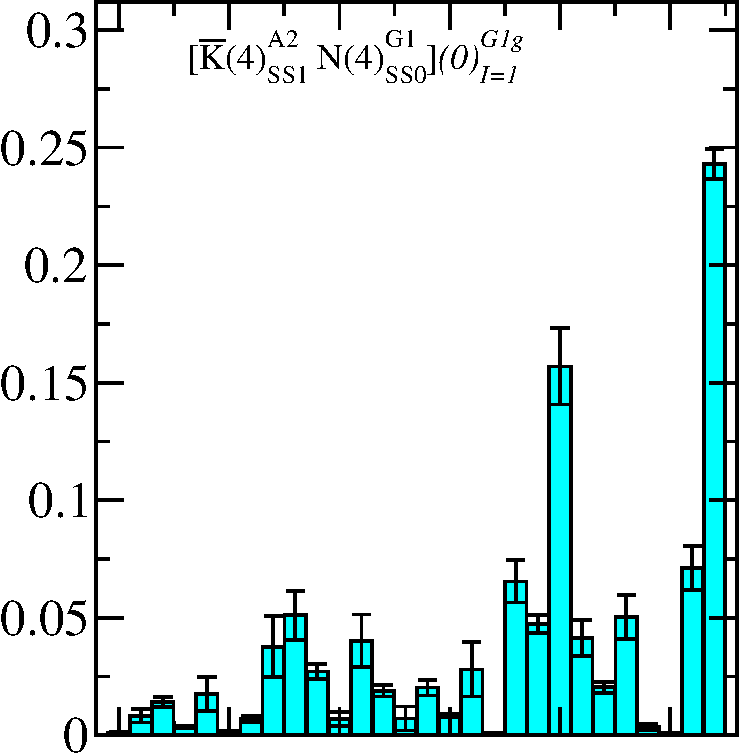
\includegraphics[width=.185\textwidth]{figures/sigmas/g1g/zfactors/zfactor_isotriplet_kbar_nucleon-G1g_1-P002-A2-SS_1-P00-2-G1-SS_0.pdf}\\
    \hspace*{-0.1cm}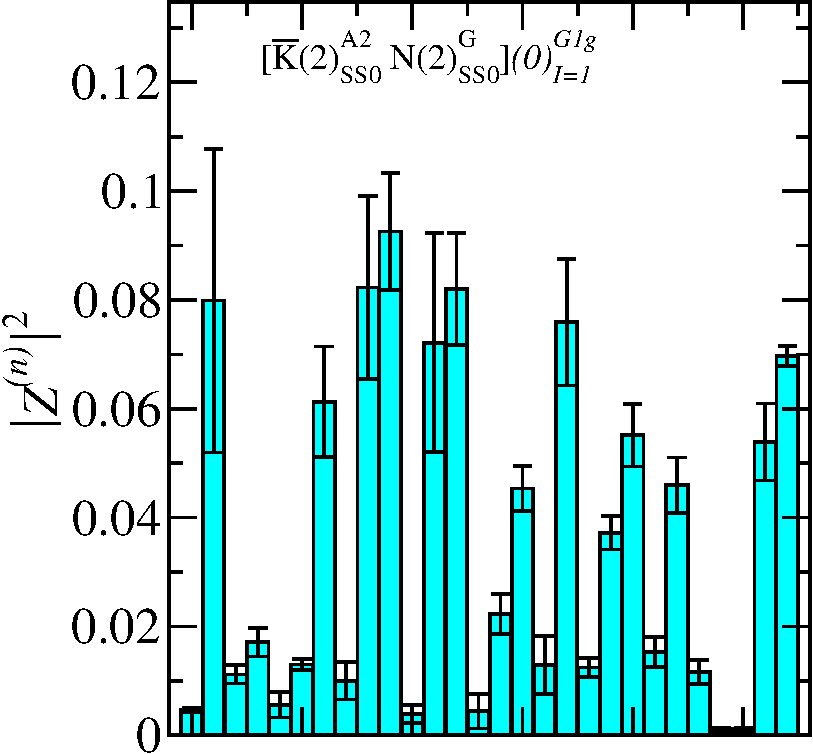
\includegraphics[width=.205\textwidth]{figures/sigmas/g1g/zfactors/zfactor_isotriplet_kbar_nucleon-G1g_1-P011-A2-SS_0-P0-1-1-G-SS_0.pdf}
    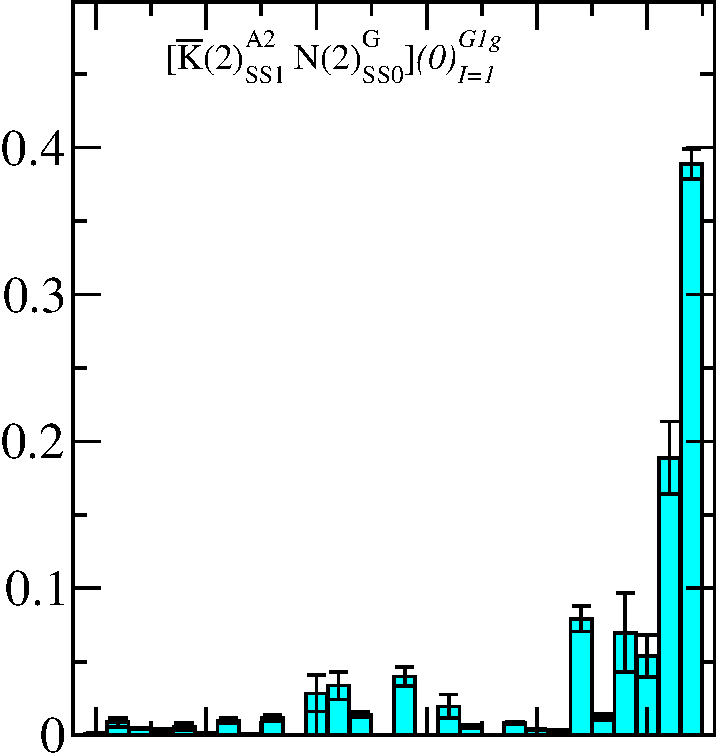
\includegraphics[width=.18\textwidth]{figures/sigmas/g1g/zfactors/zfactor_isotriplet_kbar_nucleon-G1g_1-P011-A2-SS_1-P0-1-1-G-SS_0.pdf}
    \hspace*{-0.1cm}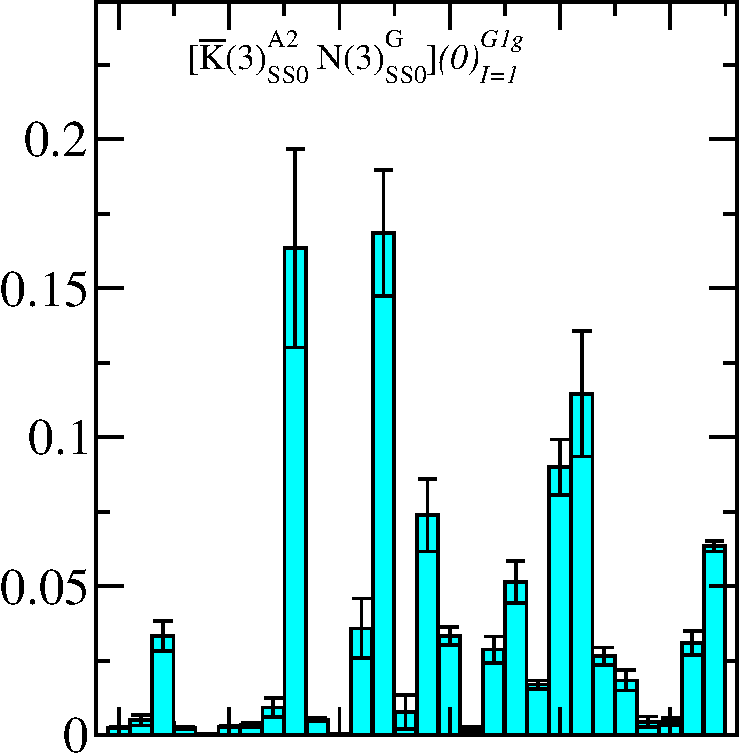
\includegraphics[width=.185\textwidth]{figures/sigmas/g1g/zfactors/zfactor_isotriplet_kbar_nucleon-G1g_1-P111-A2-SS_0-P-1-1-1-G-SS_0.pdf}
    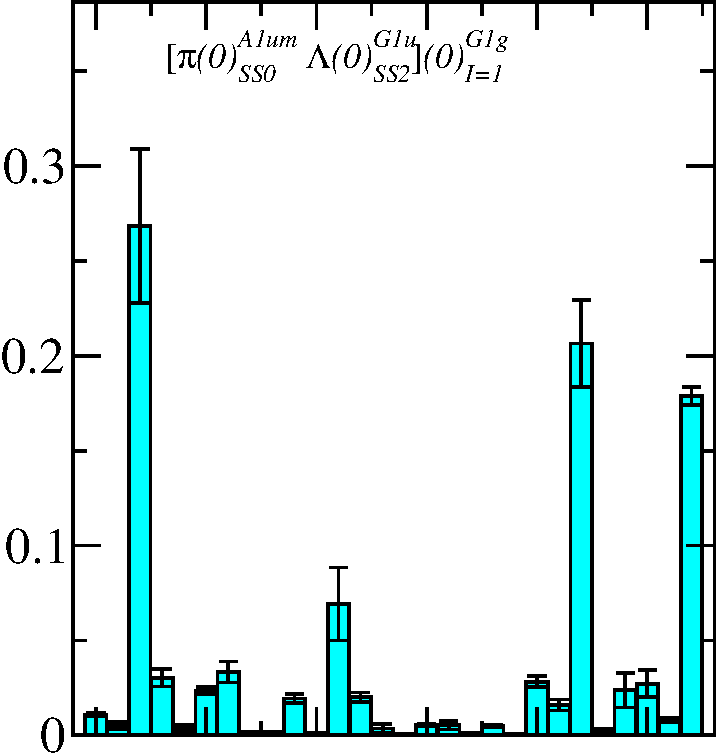
\includegraphics[width=.18\textwidth]{figures/sigmas/g1g/zfactors/zfactor_isotriplet_pion_lambda-G1g_1-P000-A1um-SS_0-P000-G1u-SS_2.pdf}
    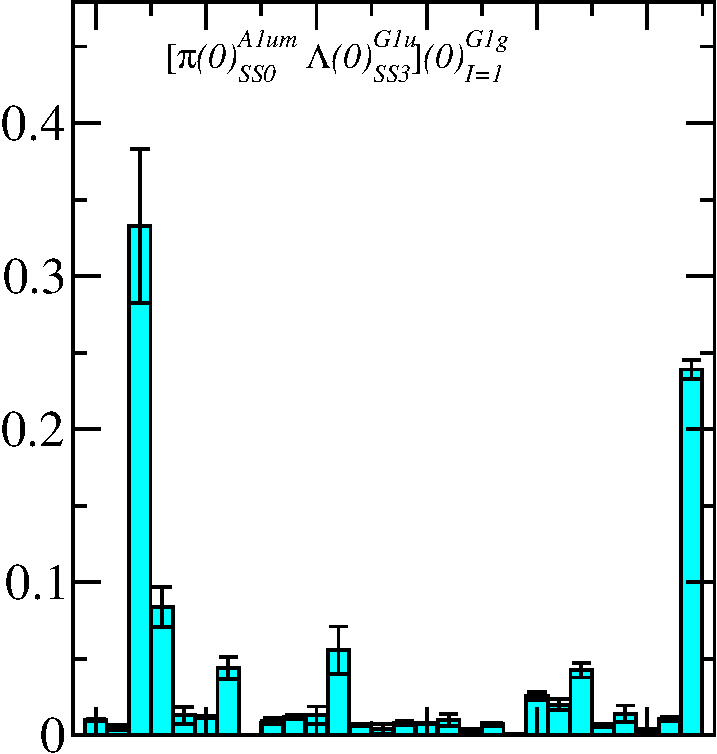
\includegraphics[width=.18\textwidth]{figures/sigmas/g1g/zfactors/zfactor_isotriplet_pion_lambda-G1g_1-P000-A1um-SS_0-P000-G1u-SS_3.pdf}\\
    \raisebox{0.5cm}{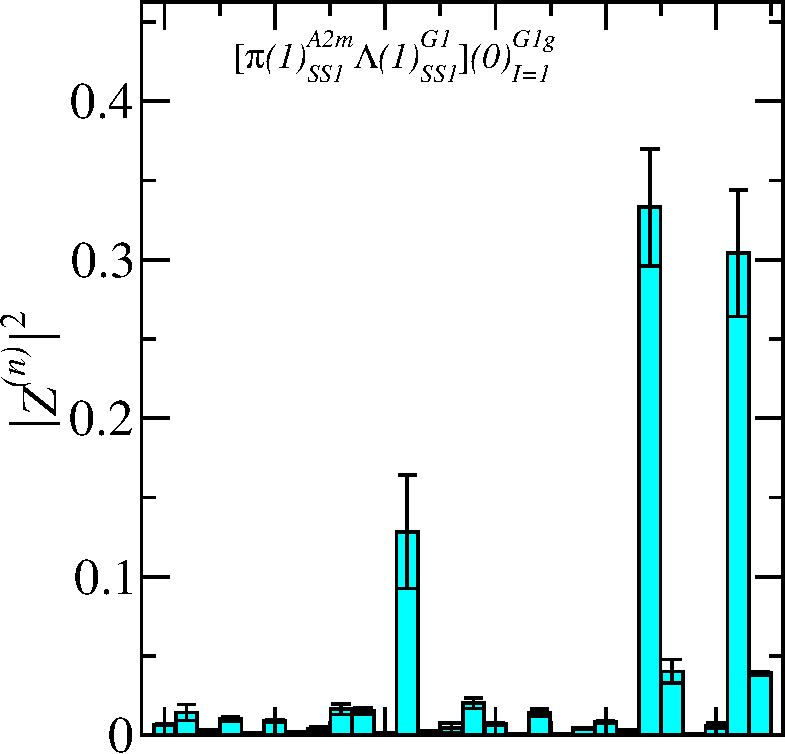
\includegraphics[width=.1975\textwidth]{figures/sigmas/g1g/zfactors/zfactor_isotriplet_pion_lambda-G1g_1-P001-A2m-SS_1-P00-1-G1-SS_1.pdf}}
    \raisebox{0.5cm}{\includegraphics[width=.18\textwidth]{figures/sigmas/g1g/zfactors/zfactor_isotriplet_pion_lambda-G1g_1-P011-A2m-SS_0-P0-1-1-G-SS_0.pdf}}
    \hspace*{-0.05cm}\raisebox{0.5cm}{\includegraphics[width=.185\textwidth]{figures/sigmas/g1g/zfactors/zfactor_isotriplet_pion_lambda-G1g_1-P111-A2m-SS_0-P-1-1-1-G-SS_0.pdf}}
    \raisebox{0.2cm}{\includegraphics[width=.18\textwidth]{figures/sigmas/g1g/zfactors/zfactor_isotriplet_pion_sigma-G1g_1-P001-A2m-SS_0-P00-1-G1-SS_0.pdf}}
    \raisebox{0.2cm}{\includegraphics[width=.18\textwidth]{figures/sigmas/g1g/zfactors/zfactor_isotriplet_pion_sigma-G1g_1-P001-A2m-SS_1-P00-1-G1-SS_0.pdf}}\\[-0.5cm]
    \includegraphics[width=.1975\textwidth]{figures/sigmas/g1g/zfactors/zfactor_isotriplet_pion_sigma-G1g_1-P001-A2m-SS_1-P00-1-G1-SS_2.pdf}
    \hspace*{-0.06cm}\includegraphics[width=.185\textwidth]{figures/sigmas/g1g/zfactors/zfactor_isotriplet_pion_sigma-G1g_1-P011-A2m-SS_0-P0-1-1-G-SS_1.pdf}
    \hspace*{-0.06cm}\includegraphics[width=.185\textwidth]{figures/sigmas/g1g/zfactors/zfactor_isotriplet_pion_sigma-G1g_1-P111-A2m-SS_0-P-1-1-1-G-SS_4.pdf}
    \caption{Overlap factors for the operators used in the rotated $28\times 28$ correlator matrix in the isotriplet $S=-1$ $G_{1g}$ symmetry channel.}\label{fig:g1g_zfactors}
\end{figure}
\renewcommand{\arraystretch}{1.2}
\begin{table}[H]
    \centering
    \begin{tabu}{c|c|c|c|c}
        $E / E_N$ & $a_t E$ & Fit model & $(t_{\mathrm{min}}, {t_\mathrm{max}})$ & $\chi^2 / \rm{d.o.f.}$\\
        \hline
        \rowfont{\color{red}}
        1.224(76)&0.2191(56)&2{-}exp&$(4, 25)$&1.34 \\
        1.81(19)&0.323(26)&2{-}exp&$(4, 20)$&1.45 \\
        1.81(13)&0.324(15)&2{-}exp&$(3, 22)$&0.96 \\
        1.82(13)&0.325(14)&2{-}exp&$(3, 25)$&1.1 \\
        1.85(20)&0.332(32)&2{-}exp&$(3, 17)$&0.98 \\
        1.90(12)&0.3403(76)&2{-}exp&$(3, 25)$&1.02 \\
        1.96(14)&0.350(16)&2{-}exp&$(3, 22)$&1.25 \\
        1.98(21)&0.355(32)&2{-}exp&$(3, 18)$&0.63 \\
        2.03(15)&0.364(20)&2{-}exp&$(3, 20)$&1.32 \\
        2.06(14)&0.369(13)&2{-}exp&$(3, 19)$&1.71 \\
        2.07(23)&0.370(36)&2{-}exp&$(3, 16)$&1.78 \\
        2.07(22)&0.371(34)&2{-}exp&$(3, 25)$&1.21 \\
        2.12(14)&0.380(13)&2{-}exp&$(3, 20)$&0.84 \\
        \rowfont{\color{red}}
        2.12(35)&0.380(59)&2{-}exp&$(3, 16)$&1.17 \\
        2.13(14)&0.381(16)&2{-}exp&$(3, 15)$&1.69 \\
        2.16(13)&0.387(11)&2{-}exp&$(3, 22)$&0.86 \\
        \rowfont{\color{red}}
        2.18(25)&0.389(39)&2{-}exp&$(3, 15)$&0.57 \\
        \rowfont{\color{red}}
        2.18(16)&0.390(19)&2{-}exp&$(3, 22)$&1.24 \\
        \rowfont{\color{red}}
        2.22(15)&0.397(15)&2{-}exp&$(3, 19)$&0.83 \\
        2.23(14)&0.3984(89)&2{-}exp&$(3, 19)$&1.29 \\
        2.25(13)&0.403(12)&2{-}exp&$(3, 21)$&1.3 \\
        2.27(18)&0.405(21)&2{-}exp&$(3, 18)$&1.59 \\
        2.28(15)&0.408(17)&1{-}exp&$(7, 17)$&1.39 \\
        \rowfont{\color{red}}
        2.30(19)&0.412(24)&1{-}exp&$(7, 17)$&1.51 \\
        2.44(27)&0.437(41)&1{-}exp&$(8, 15)$&1.32 \\
        \rowfont{\color{red}}
        2.55(23)&0.456(33)&1{-}exp&$(7, 15)$&1.16 \\
        2.63(22)&0.471(25)&1{-}exp&$(6, 15)$&0.51 \\
        3.02(18)&0.5411(75)&1{-}exp&$(3, 15)$&3.5 \\
    \end{tabu}
    \caption[Fit details for the spectrum obtained in the isotriplet $S=-1$ $G_{1g}$ symmetry channel using the operator basis given in Table~\ref{table:g1g_ops}.]{Fit details for the spectrum obtained in the isotriplet $S=-1$ $G_{1g}$ symmetry channel using the operator basis given in Table~\ref{table:g1g_ops}. Single-hadron-dominated energies are shown in red.}\label{table:g1g_fits}
\end{table}
\renewcommand{\arraystretch}{1.5}

\begin{figure}[H]
    \centering
    \hspace*{-1.5cm}\includegraphics[width=0.5\textwidth]{figures/nucleon.pdf}
    \caption{A fit to the nucleon mass, used as a reference for fits in this chapter.}\label{fig:nucleon_fit}
\end{figure}

\section{$G_{1u}$ Spectrum}
The isotriplet, $S=-1$, $G_{1u}$ symmetry channel is parity-negative and contains spins $\frac{1}{2}$, $\frac{7}{2}$, $\frac{9}{2}$, and beyond. In this channel, the only experimental resonance we expect to see is the spin-$\frac{1}{2}$ $\Sigma(1750)$. We also expect to see many multi-hadron states. We started with a basis of 10 single-hadron operators and pruned down to just 6. For the two-hadron operators, we started with a basis of 24 operators and pruned down to 20. The final basis of single- and two-hadron operators used to extract the spectrum in this channel is given in Table~\ref{table:g1u_ops}. We found that a normalization time, metric time, and diagonalization time of $\tau_N=3$, $\tau_0=4$, and $\tau_d=8$ ensured that the correlator matrix remained sufficiently diagonal.

The spectrum obtained in terms of the kaon mass is shown in Fig.~\ref{fig:g1u_spectrum}. Correlator fits are shown in Fig.~\ref{fig:g1u_fits}, and fit details are given in Table~\ref{table:g1u_fits}. A comparison of the experimentally observed $\Sigma(1750)$ resonance to the low-lying single-hadron-dominated states we obtain from the lattice is shown in Fig.~\ref{fig:g1u_exp}. As in the $G_{1g}$ channel, we do not include every single-hadron state that we extract, since we do not expect to reliably extract the masses of the higher lying states in a given channel. Our findings again seem to agree well with the results from Ref.~\cite{Edwards:2012fx}, shown in Fig.~\ref{fig:edwards}. In the Ref.~\cite{Edwards:2012fx}, they see three low-lying single-hadron states close together, followed by several higher lying states. In our comparison to experiment, we see decent agreement between the experimentally observed $\Sigma(1750)$ and our three lower lying single-hadron-dominated states.
\begin{table}[H]
    \centering
    \begin{tabular}{l|l}
        \textbf{Single-Hadron Operators} & \textbf{Two-Hadron Operators} \\
        \hline
        $\Sigma_{G_{1u}}^{DDI13}$ & $\pi(0)_{A_{1u}^-}^{SS0}\Lambda(0)_{G_{1g}}^{SS0}$\\
        $\Sigma_{G_{1u}}^{DDL34}$ & $\pi(0)_{A_{1u}^-}^{SS0}\Lambda(0)_{G_{1g}}^{SS3}$\\
        $\Sigma_{G_{1u}}^{SD5}$ & $\pi(1)_{A_2^-}^{SS0}\Lambda(1)_{G_1}^{SS1}$\\
        $\Sigma_{G_{1u}}^{SS0}$ & $\pi(1)_{A_2^-}^{SS1}\Lambda(1)_{G_1}^{SS1}$\\
        $\Sigma_{G_{1u}}^{SS2}$ & $\pi(1)_{A_2^-}^{SS1}\Lambda(1)_{G_1}^{SS2}$\\
        $\Sigma_{G_{1u}}^{TDT91}$ & $\pi(2)_{A_2^-}^{SS0}\Lambda(2)_{G}^{SS0}$\\
         & $\pi(3)_{A_2^-}^{SS0}\Lambda(3)_{G}^{SS0}$\\
         & $\pi(0)_{A_{1u}^-}^{SS0}\Sigma(0)_{G_{1g}}^{SS3}$\\
         & $\pi(1)_{A_2^-}^{SS0}\Sigma(1)_{G_1}^{SS0}$\\
         & $\pi(1)_{A_2^-}^{SS1}\Sigma(1)_{G_1}^{SS0}$\\
         & $\pi(1)_{A_2^-}^{SS1}\Sigma(1)_{G_1}^{SS2}$\\
         & $\pi(2)_{A_2^-}^{SS0}\Sigma(2)_{G}^{SS1}$\\
         & $\overline K(0)_{A_{1u}}^{SS0}N(0)_{G_{1g}}^{SS0}$\\
         & $\overline K(0)_{T_{1u}}^{SS1}N(0)_{G_{1g}}^{SS0}$\\
         & $\overline K(1)_{A_2}^{SS0}N(1)_{G_1}^{SS0}$\\
         & $\overline K(1)_{A_2}^{SS1}N(1)_{G_1}^{SS0}$\\
         & $\overline K(2)_{A_2}^{SS0}N(2)_{G}^{SS0}$\\
         & $\overline K(3)_{A_2}^{SS0}N(3)_{G}^{SS0}$\\
         & $\overline K(1)_{A_2}^{SS1}\Delta(1)_{G_1}^{SS0}$\\
         & $K(0)_{A_{1u}}^{SS0}\Xi(0)_{G_{1g}}^{SS0}$        
    \end{tabular}
    \caption{Operators used in the isotriplet $S=-1$ $G_{1u}$ symmetry sector.}\label{table:g1u_ops}
\end{table}

\begin{figure}[H]
    \centering
    \hspace*{-0.5in}\includegraphics[width=\textwidth]{figures/sigmas/g1u/staircase_mk.pdf}
    \caption[The spectrum for the isotriplet $S=-1$ $G_{1u}$ channel, obtained by fitting the energies and overlap factors of the diagonalized correlator matrix.]{The spectrum for the isotriplet $S=-1$ $G_{1u}$ channel, obtained by fitting the energies and overlap factors of the diagonalized correlator matrix. An explanation of the plot features is given in the caption of Fig.~\ref{fig:g1g_spectrum}.}\label{fig:g1u_spectrum}
\end{figure}

\begin{figure}[H]
    \centering
    \includegraphics[width=0.8\textwidth]{figures/sigmas/g1u/expvslat.pdf}
    \caption[The only experimentally observed resonance we expect to see in $G_{1u}$ compared to the finite-volume single-hadron-dominated stationary states we obtain from the lattice, in terms of the nucleon mass.]{The only experimentally observed resonance we expect to see in this channel compared to the finite-volume single-hadron-dominated stationary states we obtain from the lattice, in terms of the nucleon mass. For the experimental states, dark bands indicate experimental uncertainty and light bands indicate decay widths.}\label{fig:g1u_exp}
\end{figure}

\begin{figure}[H]
    \includegraphics[width=0.215\textwidth]{figures/sigmas/g1u/fits/fit_10.pdf}
    \includegraphics[width=0.18\textwidth]{figures/sigmas/g1u/fits/fit_0.pdf}
    \includegraphics[width=0.18\textwidth]{figures/sigmas/g1u/fits/fit_2.pdf}
    \includegraphics[width=0.18\textwidth]{figures/sigmas/g1u/fits/fit_1.pdf}
    \includegraphics[width=0.18\textwidth]{figures/sigmas/g1u/fits/fit_5.pdf}\\
    \includegraphics[width=0.215\textwidth]{figures/sigmas/g1u/fits/fit_3.pdf}
    \includegraphics[width=0.18\textwidth]{figures/sigmas/g1u/fits/fit_4.pdf}
    \includegraphics[width=0.18\textwidth]{figures/sigmas/g1u/fits/fit_9.pdf}
    \includegraphics[width=0.18\textwidth]{figures/sigmas/g1u/fits/fit_8.pdf}
    \includegraphics[width=0.18\textwidth]{figures/sigmas/g1u/fits/fit_6.pdf}\\
    \includegraphics[width=0.215\textwidth]{figures/sigmas/g1u/fits/fit_7.pdf}
    \includegraphics[width=0.18\textwidth]{figures/sigmas/g1u/fits/fit_13.pdf}
    \includegraphics[width=0.18\textwidth]{figures/sigmas/g1u/fits/fit_11.pdf}
    \includegraphics[width=0.18\textwidth]{figures/sigmas/g1u/fits/fit_15.pdf}
    \includegraphics[width=0.18\textwidth]{figures/sigmas/g1u/fits/fit_16.pdf}\\
    \raisebox{0.35cm}{\includegraphics[width=0.215\textwidth]{figures/sigmas/g1u/fits/fit_18.pdf}}
    \raisebox{0.35cm}{\includegraphics[width=0.18\textwidth]{figures/sigmas/g1u/fits/fit_12.pdf}}
    \raisebox{0.35cm}{\includegraphics[width=0.18\textwidth]{figures/sigmas/g1u/fits/fit_14.pdf}}
    \raisebox{0.35cm}{\includegraphics[width=0.18\textwidth]{figures/sigmas/g1u/fits/fit_17.pdf}}
    \includegraphics[width=0.18\textwidth]{figures/sigmas/g1u/fits/fit_20.pdf}\\[-0.35cm]
    \includegraphics[width=0.215\textwidth]{figures/sigmas/g1u/fits/fit_22.pdf}
    \includegraphics[width=0.18\textwidth]{figures/sigmas/g1u/fits/fit_19.pdf}
    \includegraphics[width=0.18\textwidth]{figures/sigmas/g1u/fits/fit_21.pdf}
    \includegraphics[width=0.18\textwidth]{figures/sigmas/g1u/fits/fit_23.pdf}
    \caption[Effective energies for the rotated $26\times 26$ correlator matrix in the isotriplet $S=-1$ $G_{1u}$ symmetry channel.]{Effective energies for the rotated $26\times 26$ correlator matrix in the isotriplet $S=-1$ $G_{1u}$ symmetry channel. Effective energy curves calculated from correlator fits are overlaid, and fit results are shown. The nucleon mass is used as a reference.}\label{fig:g1u_fits}
\end{figure}

\begin{figure}[H]
    \includegraphics[width=0.1975\textwidth]{figures/sigmas/g1u/zfactors/zfactor_isotriplet-S-1-P000-G1u_1-ROT-0.pdf}
    \includegraphics[width=0.18\textwidth]{figures/sigmas/g1u/zfactors/zfactor_isotriplet-S-1-P000-G1u_1-ROT-1.pdf}
    \includegraphics[width=0.18\textwidth]{figures/sigmas/g1u/zfactors/zfactor_isotriplet-S-1-P000-G1u_1-ROT-2.pdf}
    \includegraphics[width=0.18\textwidth]{figures/sigmas/g1u/zfactors/zfactor_isotriplet-S-1-P000-G1u_1-ROT-3.pdf}
    \includegraphics[width=0.18\textwidth]{figures/sigmas/g1u/zfactors/zfactor_isotriplet-S-1-P000-G1u_1-ROT-4.pdf}\\
    \includegraphics[width=0.1975\textwidth]{figures/sigmas/g1u/zfactors/zfactor_isotriplet-S-1-P000-G1u_1-ROT-5.pdf}
    \includegraphics[width=0.18\textwidth]{figures/sigmas/g1u/zfactors/zfactor_isotriplet_kaon_xi-G1u_1-P000-A1u-SS_0-P000-G1g-SS_0.pdf}
    \includegraphics[width=0.18\textwidth]{figures/sigmas/g1u/zfactors/zfactor_isotriplet_kbar_delta-G1u_1-P001-A2-SS_1-P00-1-G1-SS_0.pdf}
    \includegraphics[width=0.18\textwidth]{figures/sigmas/g1u/zfactors/zfactor_isotriplet_kbar_nucleon-G1u_1-P000-A1u-SS_0-P000-G1g-SS_0.pdf}
    \includegraphics[width=0.18\textwidth]{figures/sigmas/g1u/zfactors/zfactor_isotriplet_kbar_nucleon-G1u_1-P000-T1u-SS_1-P000-G1g-SS_0.pdf}\\
    \includegraphics[width=0.1975\textwidth]{figures/sigmas/g1u/zfactors/zfactor_isotriplet_kbar_nucleon-G1u_1-P001-A2-SS_0-P00-1-G1-SS_0.pdf}
    \includegraphics[width=0.18\textwidth]{figures/sigmas/g1u/zfactors/zfactor_isotriplet_kbar_nucleon-G1u_1-P001-A2-SS_1-P00-1-G1-SS_0.pdf}
    \includegraphics[width=0.18\textwidth]{figures/sigmas/g1u/zfactors/zfactor_isotriplet_kbar_nucleon-G1u_1-P011-A2-SS_0-P0-1-1-G-SS_0.pdf}
    \hspace{-0.1cm}\includegraphics[width=0.185\textwidth]{figures/sigmas/g1u/zfactors/zfactor_isotriplet_kbar_nucleon-G1u_1-P111-A2-SS_0-P-1-1-1-G-SS_0.pdf}
    \includegraphics[width=0.18\textwidth]{figures/sigmas/g1u/zfactors/zfactor_isotriplet_pion_lambda-G1u_1-P000-A1um-SS_0-P000-G1g-SS_0.pdf}\\
    \includegraphics[width=0.1975\textwidth]{figures/sigmas/g1u/zfactors/zfactor_isotriplet_pion_lambda-G1u_1-P000-A1um-SS_0-P000-G1g-SS_3.pdf}
    \includegraphics[width=0.18\textwidth]{figures/sigmas/g1u/zfactors/zfactor_isotriplet_pion_lambda-G1u_1-P001-A2m-SS_0-P00-1-G1-SS_1.pdf}
    \hspace{-0.1cm}\includegraphics[width=0.185\textwidth]{figures/sigmas/g1u/zfactors/zfactor_isotriplet_pion_lambda-G1u_1-P001-A2m-SS_1-P00-1-G1-SS_1.pdf}
    \hspace{-0.1cm}\includegraphics[width=0.185\textwidth]{figures/sigmas/g1u/zfactors/zfactor_isotriplet_pion_lambda-G1u_1-P001-A2m-SS_1-P00-1-G1-SS_2.pdf}
    \includegraphics[width=0.18\textwidth]{figures/sigmas/g1u/zfactors/zfactor_isotriplet_pion_lambda-G1u_1-P011-A2m-SS_0-P0-1-1-G-SS_0.pdf}\\
    \hspace*{-0.1cm}\raisebox{0.3cm}{\includegraphics[width=0.205\textwidth]{figures/sigmas/g1u/zfactors/zfactor_isotriplet_pion_lambda-G1u_1-P111-A2m-SS_0-P-1-1-1-G-SS_0.pdf}}
    \includegraphics[width=0.18\textwidth]{figures/sigmas/g1u/zfactors/zfactor_isotriplet_pion_sigma-G1u_1-P000-A1um-SS_0-P000-G1g-SS_3.pdf}
    \hspace{-0.1cm}\includegraphics[width=0.185\textwidth]{figures/sigmas/g1u/zfactors/zfactor_isotriplet_pion_sigma-G1u_1-P001-A2m-SS_0-P00-1-G1-SS_0.pdf}
    \hspace{-0.1cm}\includegraphics[width=0.185\textwidth]{figures/sigmas/g1u/zfactors/zfactor_isotriplet_pion_sigma-G1u_1-P001-A2m-SS_1-P00-1-G1-SS_0.pdf}
    \includegraphics[width=0.18\textwidth]{figures/sigmas/g1u/zfactors/zfactor_isotriplet_pion_sigma-G1u_1-P001-A2m-SS_1-P00-1-G1-SS_2.pdf}\\[-0.3cm]
    \hspace*{-0.1cm}\includegraphics[width=0.205\textwidth]{figures/sigmas/g1u/zfactors/zfactor_isotriplet_pion_sigma-G1u_1-P011-A2m-SS_0-P0-1-1-G-SS_1.pdf}
    \caption{Overlap factors for the operators used in the rotated $26\times 26$ correlator matrix in the isotriplet $S=-1$ $G_{1u}$ symmetry channel.}\label{fig:g1u_zfactors}
\end{figure}

\renewcommand{\arraystretch}{1.2}
\begin{table}[H]
    \centering
    \begin{tabu}{c|c|c|c|c}
        $E / E_N$ & $a_t E$ & Fit model & $(t_{\mathrm{min}}, {t_\mathrm{max}})$ & $\chi^2 / \rm{d.o.f.}$\\
        \hline
        1.60(12)&0.286(13)&2{-}exp&$(3, 25)$&0.47\\
        1.62(11)&0.290(11)&2{-}exp&$(3, 25)$&1.26\\
        1.64(12)&0.293(16)&2{-}exp&$(4, 25)$&1.05\\
        \rowfont{\color{red}}
        1.65(10)&0.2961(87)&2{-}exp&$(4, 25)$&1.27\\
        1.82(11)&0.3249(77)&2{-}exp&$(3, 25)$&1.37\\
        \rowfont{\color{red}}
        1.85(11)&0.3303(85)&2{-}exp&$(3, 25)$&1.56\\
        1.86(13)&0.334(12)&2{-}exp&$(3, 22)$&0.64\\
        1.91(13)&0.342(13)&2{-}exp&$(3, 20)$&1.22\\
        1.97(12)&0.3527(93)&2{-}exp&$(3, 24)$&1.43\\
        1.98(12)&0.3543(97)&2{-}exp&$(3, 25)$&1.64\\
        \rowfont{\color{red}}
        2.00(13)&0.358(10)&2{-}exp&$(3, 25)$&1.48\\
        2.02(17)&0.361(20)&2{-}exp&$(3, 20)$&1.53\\
        2.04(13)&0.366(12)&2{-}exp&$(3, 21)$&0.99\\
        2.09(17)&0.374(21)&2{-}exp&$(3, 17)$&0.63\\
        2.12(16)&0.379(19)&2{-}exp&$(3, 21)$&0.9\\
        2.13(28)&0.381(45)&2{-}exp&$(3, 15)$&1.3\\
        2.16(15)&0.386(16)&2{-}exp&$(3, 21)$&0.97\\
        2.25(15)&0.403(15)&2{-}exp&$(3, 19)$&1.13\\
        2.34(18)&0.418(23)&2{-}exp&$(3, 15)$&0.9\\
        2.50(20)&0.447(28)&1{-}exp&$(7, 15)$&0.93\\
        2.85(30)&0.509(46)&1{-}exp&$(7, 15)$&0.68\\
        \rowfont{\color{red}}
        2.88(18)&0.515(15)&1{-}exp&$(5, 15)$&0.38\\
        \rowfont{\color{red}}
        3.07(19)&0.549(15)&1{-}exp&$(5, 15)$&1.13\\
        \rowfont{\color{red}}
        3.16(20)&0.565(18)&1{-}exp&$(5, 15)$&0.82\\
        3.25(24)&0.582(25)&1{-}exp&$(4, 10)$&2.02\\
        3.60(22)&0.644(14)&1{-}exp&$(3, 10)$&2.42\\
    \end{tabu}
    \caption[Fit details for the spectrum obtained in the isotriplet $S=-1$ $G_{1u}$ symmetry channel using the operator basis given in Table~\ref{table:g1u_ops}.]{Fit details for the spectrum obtained in the isotriplet $S=-1$ $G_{1u}$ symmetry channel using the operator basis given in Table~\ref{table:g1u_ops}. Single-hadron-dominated energies are shown in red.}\label{table:g1u_fits}
\end{table}
\renewcommand{\arraystretch}{1.5}
\newpage
\section{$H_g$ Spectrum}
The isotriplet, $S=-1$, $H_g$ symmetry channel is parity-positive and contains spins $\frac{3}{2}$, $\frac{5}{2}$, $\frac{7}{2}$, and beyond. In addition to many multi-hadron states, we expect to see the experimentally observed $\Sigma(1385)$, $\Sigma(1915)$, and $\Sigma(2030)$ resonances, which have spins $\frac{3}{2}$, $\frac{5}{2}$, and $\frac{7}{2}$, respectively. Our initial basis contained 15 single-hadron operators, from which we pruned down to 10. We started with 33 two-hadron operators, all of which survived the pruning process and made it into the final set. The final basis of single- and two-hadron operators used to extract the spectrum in this channel is given in Table~\ref{table:hg_ops}. The normalization time, metric time, and diagonalization time used were $\tau_N=3$, $\tau_0=4$, and $\tau_d=7$. 

The spectrum obtained in terms of the kaon mass is shown in Fig.~\ref{fig:hg_spectrum}. Correlator fits are shown in Figs.~\ref{fig:hg_fits1} and~\ref{fig:hg_fits2}, and fit details are given in Tables~\ref{table:hg_fits1} and \ref{table:hg_fits2}. A comparison of the experimentally observed states in this channel to the low-lying single-hadron-dominated states we obtain from the lattice is shown in Fig.~\ref{fig:hg_exp}. As before, we do not include all of the single-hadron states in this comparison, since we cannot reliably extract the higher lying states in the spectrum. The first three single-hadron-dominated states lattice states agree within error to the experimentally observed resonances in this channel. Such a comparison cannot be taken too seriously without an extrapolation to the physical pion mass, however, which we do not do here. Our findings differ slightly from those of Ref.~\cite{Edwards:2012fx}. Comparing Fig.~\ref{fig:edwards} to Fig.~\ref{fig:hg_spectrum}, we find agreement in observing an isolated low-lying state corresponding to the $\Sigma(1385)$. Above that, Ref.~\cite{Edwards:2012fx} sees two closely grouped states, followed by a host of other states above those. In contrast to seeing two closely grouped states above the ground state, we see only one isolated single-hadron-dominated state in that region. (Above this region, we also see several other states.) We, however, see a very nearby two-hadron state with significant single-hadron mixing. This illustrates the necessity of using multi-hadron operators when performing an analysis such as this.
\begin{table}[H]
    \centering
    \begin{tabular}{l|l|l}
        \textbf{Single-Hadron Operators} & \textbf{Two-Hadron Operators} & \textbf{Two-Hadron Operators cont.}\\
        \hline
        $\Sigma_{H_g}^{DDI29}$ & $\pi(0)_{A_{1u}^-}^{SS0}\Lambda(0)_{H_u}^{SD37}$ & $\overline K(1)_{E}^{SS2}N(1)_{G_1}^{SS0}$\\
        $\Sigma_{H_g}^{DDI31}$ & $\pi(0)_{A_{1u}^-}^{SS0}\Lambda(0)_{H_u}^{SS0}$ & $\overline K(2)_{A_2}^{SS0}N(2)_{G}^{SS0}$\\
        $\Sigma_{H_g}^{DDI42}$ & $\pi(1)_{A_2^-}^{SS1}\Lambda(1)_{G_2}^{LSD1}$ & $\overline K(2)_{A_2}^{SS1}N(2)_{G}^{SS0}$\\
        $\Sigma_{H_g}^{DDL94}$ & $\pi(1)_{A_2^-}^{SS0}\Lambda(1)_{G_1}^{SS1}$ & $\overline K(1)_{A_2}^{SS1}\Delta(1)_{G_2}^{SS0}$\\
        $\Sigma_{H_g}^{SD35}$ & $\pi(1)_{A_2^-}^{SS1}\Lambda(1)_{G_1}^{SS1}$ & $\overline K(1)_{A_2}^{SS1}\Delta(1)_{G_1}^{SS0}$\\
        $\Sigma_{H_g}^{SD47}$ & $\pi(1)_{A_2^-}^{SS1}\Lambda(1)_{G_1}^{SS2}$ & $K(1)_{A_2}^{SS1}\Xi(1)_{G_1}^{SS0}$\\
        $\Sigma_{H_g}^{SS1}$ & $\pi(1)_{A_2^-}^{SS1}\Lambda(1)_{G_1}^{SS6}$ & $\eta(1)_{A_2^+}^{SS1}\Sigma(1)_{G_1}^{SS0}$\\
        $\Sigma_{H_g}^{TDT135}$ & $\pi(2)_{A_2^-}^{SS0}\Lambda(2)_{G}^{SS0}$ & \\
        $\Sigma_{H_g}^{TDT156}$ & $\pi(2)_{A_2^-}^{SS1}\Lambda(2)_{G}^{SS0}$ &\\
        $\Sigma_{H_g}^{TDT3}$ & $\pi(3)_{A_2^-}^{SS0}\Lambda(3)_{G}^{SS0}$ &\\
        & $\pi(0)_{A_{1u}^-}^{SS0}\Sigma(0)_{H_u}^{SS2}$ &\\
        & $\pi(1)_{A_2^-}^{SS1}\Sigma(1)_{G_2}^{SS0}$ &\\
        & $\pi(1)_{A_2^-}^{SS0}\Sigma(1)_{G_1}^{SS0}$ &\\
        & $\pi(1)_{A_2^-}^{SS1}\Sigma(1)_{G_1}^{SS0}$ &\\
        & $\pi(1)_{A_2^-}^{SS1}\Sigma(1)_{G_1}^{SS2}$ &\\
        & $\pi(2)_{A_2^-}^{SS0}\Sigma(2)_{G}^{SS1}$ &\\
        & $\pi(2)_{A_2^-}^{SS1}\Sigma(2)_{G}^{SS1}$ &\\
        & $\pi(3)_{A_2^-}^{SS0}\Sigma(3)_{G}^{SS4}$ &\\
        & $\overline K(1)_{E}^{SS2}N(1)_{G_1}^{SS0}$ &\\
        & $\overline K(1)_{A_1}^{SS2}N(1)_{G_1}^{SS0}$ &\\
        & $\overline K(1)_{A_2}^{SS0}N(1)_{G_1}^{SS0}$ &\\
        & $\overline K(1)_{A_2}^{SS1}N(1)_{G_1}^{SS0}$ &\\
         & $\overline K(2)_{A_2}^{SS0}N(2)_{G}^{SS0}$ &\\
         & $\overline K(2)_{A_2}^{SS1}N(2)_{G}^{SS0}$ &\\
         & $\overline K(4)_{A_2}^{SS1}N(4)_{G_1}^{SS0}$ &\\
         & $\overline K(3)_{A_2}^{SS0}N(3)_{G}^{SS0}$ &\\
    \end{tabular}
    \caption{Operators used in the isotriplet $S=-1$ $H_g$ symmetry sector.}\label{table:hg_ops}
\end{table}
\begin{figure}[H]
    \centering
    \hspace*{-0.5in}\includegraphics[width=\textwidth]{figures/sigmas/hg/staircase_mk.pdf}
    \caption[The spectrum for the isotriplet $S=-1$ $H_g$ channel, obtained by fitting the energies and overlap factors of the diagonalized correlator matrix.]{The spectrum for the isotriplet $S=-1$ $H_g$ channel, obtained by fitting the energies and overlap factors of the diagonalized correlator matrix. An explanation of the plot features is given in the caption of Fig.~\ref{fig:g1g_spectrum}.}\label{fig:hg_spectrum}
\end{figure}

\begin{figure}[H]
    \centering
    \includegraphics[width=0.8\textwidth]{figures/sigmas/hg/expvslat.pdf}
    \caption[Experimentally observed resonances compared with the finite-volume single-hadron-dominated stationary states we obtain from the lattice in $H_g$, in terms of the nucleon mass.]{Experimentally observed resonances compared with the finite-volume single-hadron-dominated stationary states we obtain from the lattice, in terms of the nucleon mass. For the experimental states, dark bands indicate experimental uncertainty and light bands indicate decay widths.}\label{fig:hg_exp}
\end{figure}

\begin{figure}[H]
    \raisebox{-0.063cm}{\includegraphics[width=0.215\textwidth]{figures/sigmas/hg/fits/fit_0.pdf}}
    \includegraphics[width=0.18\textwidth]{figures/sigmas/hg/fits/fit_2.pdf}
    \includegraphics[width=0.18\textwidth]{figures/sigmas/hg/fits/fit_4.pdf}
    \includegraphics[width=0.18\textwidth]{figures/sigmas/hg/fits/fit_6.pdf}
    \includegraphics[width=0.18\textwidth]{figures/sigmas/hg/fits/fit_5.pdf}\\
    \raisebox{-0.063cm}{\includegraphics[width=0.215\textwidth]{figures/sigmas/hg/fits/fit_10.pdf}}
    \includegraphics[width=0.18\textwidth]{figures/sigmas/hg/fits/fit_1.pdf}
    \includegraphics[width=0.18\textwidth]{figures/sigmas/hg/fits/fit_11.pdf}
    \includegraphics[width=0.18\textwidth]{figures/sigmas/hg/fits/fit_14.pdf}
    \includegraphics[width=0.18\textwidth]{figures/sigmas/hg/fits/fit_30.pdf}\\
    \raisebox{-0.063cm}{\includegraphics[width=0.215\textwidth]{figures/sigmas/hg/fits/fit_12.pdf}}
    \includegraphics[width=0.18\textwidth]{figures/sigmas/hg/fits/fit_3.pdf}
    \includegraphics[width=0.18\textwidth]{figures/sigmas/hg/fits/fit_8.pdf}
    \includegraphics[width=0.18\textwidth]{figures/sigmas/hg/fits/fit_9.pdf}
    \includegraphics[width=0.18\textwidth]{figures/sigmas/hg/fits/fit_18.pdf}\\
    \raisebox{-0.063cm}{\includegraphics[width=0.215\textwidth]{figures/sigmas/hg/fits/fit_23.pdf}}
    \includegraphics[width=0.18\textwidth]{figures/sigmas/hg/fits/fit_31.pdf}
    \includegraphics[width=0.18\textwidth]{figures/sigmas/hg/fits/fit_33.pdf}
    \includegraphics[width=0.18\textwidth]{figures/sigmas/hg/fits/fit_13.pdf}
    \includegraphics[width=0.18\textwidth]{figures/sigmas/hg/fits/fit_22.pdf}\\
    \raisebox{-0.063cm}{\includegraphics[width=0.215\textwidth]{figures/sigmas/hg/fits/fit_15.pdf}}
    \includegraphics[width=0.18\textwidth]{figures/sigmas/hg/fits/fit_26.pdf}
    \includegraphics[width=0.18\textwidth]{figures/sigmas/hg/fits/fit_16.pdf}
    \includegraphics[width=0.18\textwidth]{figures/sigmas/hg/fits/fit_20.pdf}
    \includegraphics[width=0.18\textwidth]{figures/sigmas/hg/fits/fit_17.pdf}\\
    \includegraphics[width=0.215\textwidth]{figures/sigmas/hg/fits/fit_28.pdf}
    \includegraphics[width=0.18\textwidth]{figures/sigmas/hg/fits/fit_32.pdf}
    \includegraphics[width=0.18\textwidth]{figures/sigmas/hg/fits/fit_39.pdf}
    \includegraphics[width=0.18\textwidth]{figures/sigmas/hg/fits/fit_27.pdf}
    \includegraphics[width=0.18\textwidth]{figures/sigmas/hg/fits/fit_29.pdf}
    \caption[The first 30 effective energies for the rotated $43\times 43$ correlator matrix in the isotriplet $S=-1$ $H_g$ symmetry channel.]{The first 30 effective energies for the rotated $43\times 43$ correlator matrix in the isotriplet $S=-1$ $H_g$ symmetry channel. Effective energy curves calculated from correlator fits are overlaid, and fit results are shown. The nucleon mass is used as a reference.}\label{fig:hg_fits1}
\end{figure}

\begin{figure}[H]
    \raisebox{-0.063cm}{\includegraphics[width=0.215\textwidth]{figures/sigmas/hg/fits/fit_25.pdf}}
    \includegraphics[width=0.18\textwidth]{figures/sigmas/hg/fits/fit_19.pdf}
    \includegraphics[width=0.18\textwidth]{figures/sigmas/hg/fits/fit_7.pdf}
    \includegraphics[width=0.18\textwidth]{figures/sigmas/hg/fits/fit_21.pdf}
    \includegraphics[width=0.18\textwidth]{figures/sigmas/hg/fits/fit_24.pdf}\\
    \raisebox{0.5cm}{\includegraphics[width=0.215\textwidth]{figures/sigmas/hg/fits/fit_34.pdf}}
    \raisebox{0.56cm}{\includegraphics[width=0.18\textwidth]{figures/sigmas/hg/fits/fit_35.pdf}}
    \raisebox{0.56cm}{\includegraphics[width=0.18\textwidth]{figures/sigmas/hg/fits/fit_42.pdf}}
    \raisebox{0.22cm}{\includegraphics[width=0.18\textwidth]{figures/sigmas/hg/fits/fit_40.pdf}}
    \raisebox{0.22cm}{\includegraphics[width=0.18\textwidth]{figures/sigmas/hg/fits/fit_38.pdf}}\\[-0.5cm]
    \includegraphics[width=0.215\textwidth]{figures/sigmas/hg/fits/fit_36.pdf}
    \includegraphics[width=0.18\textwidth]{figures/sigmas/hg/fits/fit_37.pdf}
    \includegraphics[width=0.18\textwidth]{figures/sigmas/hg/fits/fit_41.pdf}
    \caption[The rest of the effective energies for the rotated $43\times 43$ correlator matrix in the isotriplet $S=-1$ $H_g$ symmetry channel.]{The rest of the effective energies for the rotated $43\times 43$ correlator matrix in the isotriplet $S=-1$ $H_g$ symmetry channel. Effective energy curves calculated from correlator fits are overlaid, and fit results are shown. The nucleon mass is used as a reference.}\label{fig:hg_fits2}
\end{figure}

\begin{figure}[H]
    \includegraphics[width=0.1975\textwidth]{figures/sigmas/hg/zfactors/zfactor_isotriplet-S-1-P000-Hg_1-ROT-0.pdf}
    \includegraphics[width=0.185\textwidth]{figures/sigmas/hg/zfactors/zfactor_isotriplet-S-1-P000-Hg_1-ROT-1.pdf}
    \includegraphics[width=0.18\textwidth]{figures/sigmas/hg/zfactors/zfactor_isotriplet-S-1-P000-Hg_1-ROT-2.pdf}
    \includegraphics[width=0.185\textwidth]{figures/sigmas/hg/zfactors/zfactor_isotriplet-S-1-P000-Hg_1-ROT-3.pdf}
    \includegraphics[width=0.18\textwidth]{figures/sigmas/hg/zfactors/zfactor_isotriplet-S-1-P000-Hg_1-ROT-4.pdf}\\
    \hspace*{-0.1cm}\includegraphics[width=0.205\textwidth]{figures/sigmas/hg/zfactors/zfactor_isotriplet-S-1-P000-Hg_1-ROT-5.pdf}
    \hspace*{0.075cm}\includegraphics[width=0.18\textwidth]{figures/sigmas/hg/zfactors/zfactor_isotriplet-S-1-P000-Hg_1-ROT-6.pdf}
    \hspace*{-0.1cm}\includegraphics[width=0.185\textwidth]{figures/sigmas/hg/zfactors/zfactor_isotriplet-S-1-P000-Hg_1-ROT-7.pdf}
    \hspace*{0.1cm}\includegraphics[width=0.18\textwidth]{figures/sigmas/hg/zfactors/zfactor_isotriplet-S-1-P000-Hg_1-ROT-8.pdf}
    \includegraphics[width=0.18\textwidth]{figures/sigmas/hg/zfactors/zfactor_isotriplet-S-1-P000-Hg_1-ROT-9.pdf}\\
    \hspace*{-0.1cm}\includegraphics[width=0.205\textwidth]{figures/sigmas/hg/zfactors/zfactor_isotriplet_eta_sigma-Hg_1-P010-A2p-SS_1-P0-10-G1-SS_0.pdf}
    \includegraphics[width=0.185\textwidth]{figures/sigmas/hg/zfactors/zfactor_isotriplet_kaon_xi-Hg_1-P010-A2-SS_1-P0-10-G1-SS_0.pdf}
    \hspace*{-0.1cm}\includegraphics[width=0.185\textwidth]{figures/sigmas/hg/zfactors/zfactor_isotriplet_kbar_delta-Hg_1-P001-A2-SS_1-P00-1-G2-SS_0.pdf}
    \includegraphics[width=0.185\textwidth]{figures/sigmas/hg/zfactors/zfactor_isotriplet_kbar_delta-Hg_1-P010-A2-SS_1-P0-10-G1-SS_0.pdf}
    \hspace*{-0.075cm}\includegraphics[width=0.185\textwidth]{figures/sigmas/hg/zfactors/zfactor_isotriplet_kbar_nucleon-Hg_1-CG_1-P001-E-SS_2-P00-1-G1-SS_0.pdf}\\
    \hspace*{-0.1cm}\includegraphics[width=0.205\textwidth]{figures/sigmas/hg/zfactors/zfactor_isotriplet_kbar_nucleon-Hg_1-CG_1-P011-A2-SS_0-P0-1-1-G-SS_0.pdf}
    \hspace*{0.1cm}\includegraphics[width=0.18\textwidth]{figures/sigmas/hg/zfactors/zfactor_isotriplet_kbar_nucleon-Hg_1-CG_1-P011-A2-SS_1-P0-1-1-G-SS_0.pdf}
    \hspace*{-0.1cm}\includegraphics[width=0.185\textwidth]{figures/sigmas/hg/zfactors/zfactor_isotriplet_kbar_nucleon-Hg_1-P001-E-SS_2-P00-1-G1-SS_0.pdf}
    \includegraphics[width=0.185\textwidth]{figures/sigmas/hg/zfactors/zfactor_isotriplet_kbar_nucleon-Hg_1-P010-A1-SS_2-P0-10-G1-SS_0.pdf}
    \includegraphics[width=0.18\textwidth]{figures/sigmas/hg/zfactors/zfactor_isotriplet_kbar_nucleon-Hg_1-P010-A2-SS_0-P0-10-G1-SS_0.pdf}\\
    \includegraphics[width=0.20\textwidth]{figures/sigmas/hg/zfactors/zfactor_isotriplet_kbar_nucleon-Hg_1-P010-A2-SS_1-P0-10-G1-SS_0.pdf}
    \includegraphics[width=0.18\textwidth]{figures/sigmas/hg/zfactors/zfactor_isotriplet_kbar_nucleon-Hg_1-P011-A2-SS_0-P0-1-1-G-SS_0.pdf}
    \hspace*{0.1cm}\includegraphics[width=0.18\textwidth]{figures/sigmas/hg/zfactors/zfactor_isotriplet_kbar_nucleon-Hg_1-P011-A2-SS_1-P0-1-1-G-SS_0.pdf}
    \hspace*{-0.05cm}\includegraphics[width=0.185\textwidth]{figures/sigmas/hg/zfactors/zfactor_isotriplet_kbar_nucleon-Hg_1-P020-A2-SS_1-P0-20-G1-SS_0.pdf}
    \includegraphics[width=0.185\textwidth]{figures/sigmas/hg/zfactors/zfactor_isotriplet_kbar_nucleon-Hg_1-P111-A2-SS_0-P-1-1-1-G-SS_0.pdf}\\
    \hspace*{-0.1cm}\includegraphics[width=0.206\textwidth]{figures/sigmas/hg/zfactors/zfactor_isotriplet_pion_lambda-Hg_1-P000-A1um-SS_0-P000-Hu-SD_37.pdf}
    \hspace*{-0.05cm}\includegraphics[width=0.185\textwidth]{figures/sigmas/hg/zfactors/zfactor_isotriplet_pion_lambda-Hg_1-P000-A1um-SS_0-P000-Hu-SS_0.pdf}
    \includegraphics[width=0.185\textwidth]{figures/sigmas/hg/zfactors/zfactor_isotriplet_pion_lambda-Hg_1-P001-A2m-SS_1-P00-1-G2-LSD_1.pdf}
    \includegraphics[width=0.18\textwidth]{figures/sigmas/hg/zfactors/zfactor_isotriplet_pion_lambda-Hg_1-P010-A2m-SS_0-P0-10-G1-SS_1.pdf}
    \includegraphics[width=0.185\textwidth]{figures/sigmas/hg/zfactors/zfactor_isotriplet_pion_lambda-Hg_1-P010-A2m-SS_1-P0-10-G1-SS_1.pdf}
    \caption{Overlap factors for the first 30 operators in our $43\times 43$ correlator matrix in the isotriplet $S=-1$ $H_g$ symmetry channel.}\label{fig:hg_zfactors1}
\end{figure}

\begin{figure}[H]
    \includegraphics[width=0.205\textwidth]{figures/sigmas/hg/zfactors/zfactor_isotriplet_pion_lambda-Hg_1-P010-A2m-SS_1-P0-10-G1-SS_2.pdf}
    \includegraphics[width=0.185\textwidth]{figures/sigmas/hg/zfactors/zfactor_isotriplet_pion_lambda-Hg_1-P010-A2m-SS_1-P0-10-G1-SS_6.pdf}
    \includegraphics[width=0.185\textwidth]{figures/sigmas/hg/zfactors/zfactor_isotriplet_pion_lambda-Hg_1-P011-A2m-SS_0-P0-1-1-G-SS_0.pdf}
    \includegraphics[width=0.185\textwidth]{figures/sigmas/hg/zfactors/zfactor_isotriplet_pion_lambda-Hg_1-P011-A2m-SS_1-P0-1-1-G-SS_0.pdf}
    \includegraphics[width=0.185\textwidth]{figures/sigmas/hg/zfactors/zfactor_isotriplet_pion_lambda-Hg_1-P111-A2m-SS_0-P-1-1-1-G-SS_0.pdf}\\
    \raisebox{0.25cm}{\includegraphics[width=0.205\textwidth]{figures/sigmas/hg/zfactors/zfactor_isotriplet_pion_sigma-Hg_1-P000-A1um-SS_0-P000-Hu-SS_2.pdf}}
    \raisebox{0.25cm}{\includegraphics[width=0.186\textwidth]{figures/sigmas/hg/zfactors/zfactor_isotriplet_pion_sigma-Hg_1-P001-A2m-SS_1-P00-1-G2-SS_0.pdf}}
    \hspace*{0.1cm}\raisebox{0.25cm}{\includegraphics[width=0.18\textwidth]{figures/sigmas/hg/zfactors/zfactor_isotriplet_pion_sigma-Hg_1-P010-A2m-SS_0-P0-10-G1-SS_0.pdf}}
    \hspace*{0.05cm}\includegraphics[width=0.18\textwidth]{figures/sigmas/hg/zfactors/zfactor_isotriplet_pion_sigma-Hg_1-P010-A2m-SS_1-P0-10-G1-SS_0.pdf}
    \includegraphics[width=0.186\textwidth]{figures/sigmas/hg/zfactors/zfactor_isotriplet_pion_sigma-Hg_1-P010-A2m-SS_1-P0-10-G1-SS_2.pdf}\\[-0.2cm]
    \includegraphics[width=0.205\textwidth]{figures/sigmas/hg/zfactors/zfactor_isotriplet_pion_sigma-Hg_1-P011-A2m-SS_0-P0-1-1-G-SS_1.pdf}
    \includegraphics[width=0.187\textwidth]{figures/sigmas/hg/zfactors/zfactor_isotriplet_pion_sigma-Hg_1-P011-A2m-SS_1-P0-1-1-G-SS_1.pdf}
    \includegraphics[width=0.185\textwidth]{figures/sigmas/hg/zfactors/zfactor_isotriplet_pion_sigma-Hg_1-P111-A2m-SS_0-P-1-1-1-G-SS_4.pdf}
    \caption{Overlap factors for the rest of the operators in our $43\times 43$ correlator matrix in the isotriplet $S=-1$ $H_g$ symmetry channel.}\label{fig:hg_zfactors2}
\end{figure}

\newpage
\renewcommand{\arraystretch}{1.2}
\begin{table}[H]
    \centering
    \begin{tabu}{c|c|c|c|c}
        $E / E_N$ & $a_t E$ & Fit model & $(t_{\mathrm{min}}, {t_\mathrm{max}})$ & $\chi^2 / \rm{d.o.f.}$\\
        \hline
        \rowfont{\color{red}}
        1.540(98)&0.2755(69)&2{-}exp&$(4, 25)$&0.64 \\
        1.83(17)&0.327(27)&2{-}exp&$(3, 25)$&2.85 \\
        1.84(12)&0.330(11)&1{-}exp&$(10, 22)$&0.94 \\
        1.92(12)&0.344(11)&1{-}exp&$(10, 25)$&0.99 \\
        1.94(15)&0.348(20)&2{-}exp&$(3, 25)$&1.72 \\
        1.99(14)&0.356(14)&2{-}exp&$(3, 21)$&1.55 \\
        2.01(15)&0.360(15)&1{-}exp&$(8, 20)$&1.06 \\
        2.02(17)&0.361(22)&1{-}exp&$(11, 21)$&0.88 \\
        2.07(13)&0.371(11)&1{-}exp&$(8, 20)$&1.23 \\
        2.09(16)&0.375(20)&1{-}exp&$(9, 19)$&0.58 \\
        2.10(13)&0.376(10)&2{-}exp&$(3, 20)$&1.69 \\
        2.10(15)&0.376(16)&2{-}exp&$(3, 25)$&1.32 \\
        2.12(14)&0.379(13)&1{-}exp&$(9, 20)$&0.96 \\
        \rowfont{\color{red}}
        2.12(13)&0.3801(96)&2{-}exp&$(3, 21)$&1.57 \\
        2.13(17)&0.382(20)&2{-}exp&$(3, 18)$&1.15 \\
        2.14(21)&0.383(31)&2{-}exp&$(3, 16)$&1.07 \\
        2.19(23)&0.392(33)&2{-}exp&$(3, 16)$&1.0 \\
        2.20(27)&0.394(42)&2{-}exp&$(3, 16)$&0.56 \\
        2.26(15)&0.404(12)&2{-}exp&$(3, 22)$&1.16 \\
        2.26(17)&0.405(19)&2{-}exp&$(3, 18)$&0.82 \\
        2.27(14)&0.407(11)&2{-}exp&$(3, 21)$&0.81 \\
        2.30(15)&0.413(14)&2{-}exp&$(3, 22)$&0.53 \\
        2.31(14)&0.413(11)&2{-}exp&$(3, 22)$&1.28 \\
        2.33(16)&0.417(17)&2{-}exp&$(3, 20)$&0.85 \\
        \rowfont{\color{red}}
        2.34(15)&0.418(12)&2{-}exp&$(3, 19)$&1.02 \\
        \rowfont{\color{red}}
        2.35(19)&0.421(26)&2{-}exp&$(3, 16)$&0.32 \\
        \rowfont{\color{red}}
        2.37(16)&0.425(14)&1{-}exp&$(7, 19)$&1.37
    \end{tabu}
    \caption[Fit details for the first 27 fits in the spectrum obtained in the isotriplet $S=-1$ $H_g$ symmetry channel using the operator basis given in Table~\ref{table:hg_ops}.]{Fit details for the first 27 fits in the spectrum obtained in the isotriplet $S=-1$ $H_g$ symmetry channel using the operator basis given in Table~\ref{table:hg_ops}. Single-hadron-dominated energies are shown in red.}\label{table:hg_fits1}
\end{table}

\begin{table}[H]
    \centering
    \begin{tabu}{c|c|c|c|c}
        $E / E_N$ & $a_t E$ & Fit model & $(t_{\mathrm{min}}, {t_\mathrm{max}})$ & $\chi^2 / \rm{d.o.f.}$\\
        \hline
        2.38(21)&0.426(29)&1{-}exp&$(7, 15)$&1.06 \\
        2.39(14)&0.428(12)&1{-}exp&$(7, 15)$&0.28 \\
        2.43(15)&0.435(13)&1{-}exp&$(7, 16)$&0.85 \\
        2.44(16)&0.436(13)&1{-}exp&$(7, 15)$&0.98 \\
        \rowfont{\color{red}}
        2.44(14)&0.4362(79)&1{-}exp&$(6, 20)$&0.95 \\
        2.48(14)&0.4440(53)&1{-}exp&$(5, 20)$&1.17 \\
        \rowfont{\color{red}}
        2.49(15)&0.445(12)&2{-}exp&$(3, 19)$&0.84 \\
        \rowfont{\color{red}}
        2.50(14)&0.4481(93)&1{-}exp&$(6, 22)$&1.22 \\
        2.55(18)&0.456(19)&1{-}exp&$(7, 18)$&1.18 \\
        \rowfont{\color{red}}
        2.62(21)&0.469(27)&1{-}exp&$(7, 17)$&0.38 \\
        2.64(33)&0.473(54)&1{-}exp&$(8, 15)$&0.54 \\
        2.71(33)&0.484(50)&1{-}exp&$(8, 14)$&1.76 \\
        2.78(20)&0.498(22)&1{-}exp&$(6, 15)$&1.22 \\
        2.79(24)&0.499(29)&1{-}exp&$(7, 15)$&0.77 \\
        \rowfont{\color{red}}
        3.03(20)&0.542(15)&1{-}exp&$(5, 15)$&1.35 \\
        3.48(31)&0.622(42)&1{-}exp&$(6, 14)$&2.16 \\
    \end{tabu}
    \caption[Fit details for the rest of the fits in the spectrum obtained in the isotriplet $S=-1$ $H_g$ symmetry channel using the operator basis given in Table~\ref{table:hg_ops}.]{Fit details for the rest of the fits in the spectrum obtained in the isotriplet $S=-1$ $H_g$ symmetry channel using the operator basis given in Table~\ref{table:hg_ops}. Single-hadron-dominated energies are shown in red.}\label{table:hg_fits2}
\end{table}
\renewcommand{\arraystretch}{1.5}

\newpage
\section{$H_u$ Spectrum}
The isotriplet, $S=-1$, $H_u$ symmetry channel is parity-negative and consists of spins $\frac{3}{2}$, $\frac{5}{2}$, $\frac{7}{2}$, and beyond. In addition to many multi-hadron states, we expect to see the experimentally observed $\Sigma(1670)$, $\Sigma(1775)$, and $\Sigma(1940)$, which have spins $\frac{3}{2}$, $\frac{5}{2}$, and $\frac{3}{2}$, respectively. Our initial basis contained 14 single-hadron operators, and we pruned down to a set of just 7. We started with 27 two-hadron operators, and pruned down to 25. The final basis of single- and two-hadron operators used to extract the spectrum in this channel is given in Table~\ref{table:hu_ops}. The normalization time, metric time, and diagonalization time used were $\tau_N=3$, $\tau_0=4$, and $\tau_d=8$.

The spectrum obtained in terms of the kaon mass is shown in Fig.~\ref{fig:hu_spectrum}. A comparison to the experimentally observed states in this channel to the low-lying single-hadron-dominated states we obtain from the lattice is shown in Fig.~\ref{fig:hu_exp}. As in previous channels, higher lying states which we cannot reliably extract are excluded from this plot. We observe statistical agreement between the first three experimental resonances and the first three single-hadron-dominated finite-volume states in our spectrum. Again, we cannot take such a comparison too seriously without a physical-point extrapolation of the pion mass. The pattern of single-hadron-dominated states we observe also seems to qualitatively agree with that obtained by Ref.~\cite{Edwards:2012fx}: We see four low-lying states, followed by higher-lying states in a region where we cannot confidently extract the spectrum.

\begin{table}[H]
    \centering
    \begin{tabular}{l|l}
        \textbf{Single-Hadron Operators} & \textbf{Two-Hadron Operators} \\
        \hline
        $\Sigma_{H_u}^{DDI10}$ & $\pi(0)_{T_{1u}^+}^{SS0}\Lambda(0)_{G_{1g}}^{SS0}$\\
        $\Sigma_{H_u}^{DDI15}$ & $\pi(1)_{A_2^-}^{SS0}\Lambda(1)_{G_1}^{SS1}$\\
        $\Sigma_{H_u}^{SD44}$ & $\pi(1)_{A_2^-}^{SS1}\Lambda(1)_{G_1}^{SS1}$\\
        $\Sigma_{H_u}^{SS0}$ & $\pi(1)_{A_2^-}^{SS1}\Lambda(1)_{G_1}^{SS2}$\\
        $\Sigma_{H_u}^{TDT190}$ & $\pi(2)_{A_2^-}^{SS0}\Lambda(2)_{G}^{SS0}$\\
        $\Sigma_{H_u}^{TDT41}$ & $\pi(3)_{A_2^-}^{SS0}\Lambda(3)_{G}^{SS0}$\\
        $\Sigma_{H_u}^{TDT5}$ & $\pi(2)_{A_2^-}^{SS0}\Lambda(2)_{G}^{SS0}$\\
        & $\pi(0)_{A_{1u}^-}^{SS0}\Sigma(0)_{H_g}^{SS0}$\\
        & $\pi(0)_{A_{1u}^-}^{TDO1}\Sigma(0)_{H_g}^{SS0}$\\
        & $\pi(1)_{A_2^-}^{SS1}\Sigma(1)_{G_2}^{SS0}$\\
        & $\pi(1)_{A_2^-}^{SS0}\Sigma(1)_{G_1}^{SS0}$\\
        & $\pi(1)_{A_2^-}^{SS1}\Sigma(1)_{G_1}^{SS0}$\\
        & $\pi(1)_{A_2^-}^{SS1}\Sigma(1)_{G_1}^{SS2}$\\
        & $\pi(2)_{A_2^-}^{SS0}\Sigma(2)_{G}^{SS1}$\\
        & $\overline K(0)_{T_{1u}}^{SS1}N(0)_{G_{1g}}^{SS0}$\\
        & $\overline K(1)_{A_2}^{SS0}N(1)_{G_1}^{SS0}$\\
        & $\overline K(1)_{A_2}^{SS1}N(1)_{G_1}^{SS0}$\\
        & $\overline K(2)_{A_2}^{SS0}N(2)_{G}^{SS0}$\\
        & $\overline K(2)_{A_2}^{SS1}N(2)_{G}^{SS0}$\\
        & $\overline K(3)_{A_2}^{SS0}N(3)_{G}^{SS0}$\\
        & $\overline K(2)_{A_2}^{SS0}N(2)_{G}^{SS0}$\\
        & $\overline K(0)_{A_{1u}}^{SS0}\Delta(0)_{H_g}^{SS0}$\\
        & $\overline K(1)_{A_2}^{SS1}\Delta(1)_{G_2}^{SS0}$\\
        & $\overline K(1)_{A_2}^{SS1}\Delta(1)_{G_1}^{SS0}$\\
        & $\eta(1)_{A_2^+}^{SS1}\Sigma(1)_{G_1}^{SS0}$
    \end{tabular}
    \caption{Operators used in the isotriplet $S=-1$ $H_u$ symmetry sector.}\label{table:hu_ops}
\end{table}

\begin{figure}[H]
    \centering
    \hspace*{-0.5in}\includegraphics[width=\textwidth]{figures/sigmas/hu/staircase_mk.pdf}
    \caption[The spectrum for the isotriplet $S=-1$ $H_u$ channel, obtained by fitting the energies and overlap factors of the diagonalized correlator matrix.]{The spectrum for the isotriplet $S=-1$ $H_u$ channel, obtained by fitting the energies and overlap factors of the diagonalized correlator matrix. An explanation of the plot features is given in the caption of Fig.~\ref{fig:g1g_spectrum}.}\label{fig:hu_spectrum}
\end{figure}

\begin{figure}[H]
    \centering
    \includegraphics[width=0.8\textwidth]{figures/sigmas/hu/expvslat.pdf}
    \caption[Experimentally observed resonances compared with the finite-volume single-hadron-dominated stationary states we obtain from the lattice in $H_u$, in terms of the nucleon mass.]{Experimentally observed resonances compared with the finite-volume single-hadron-dominated stationary states we obtain from the lattice, in terms of the nucleon mass. For the experimental states, dark bands indicate experimental uncertainty and light bands indicate decay widths.}\label{fig:hu_exp}
\end{figure}

\begin{figure}[H]
    \raisebox{-0.07cm}{\includegraphics[width=0.215\textwidth]{figures/sigmas/hu/fits/fit_4.pdf}}
    \includegraphics[width=0.18\textwidth]{figures/sigmas/hu/fits/fit_0.pdf}
    \includegraphics[width=0.18\textwidth]{figures/sigmas/hu/fits/fit_8.pdf}
    \includegraphics[width=0.18\textwidth]{figures/sigmas/hu/fits/fit_3.pdf}
    \includegraphics[width=0.18\textwidth]{figures/sigmas/hu/fits/fit_1.pdf}\\
    \raisebox{-0.07cm}{\includegraphics[width=0.215\textwidth]{figures/sigmas/hu/fits/fit_13.pdf}}
    \includegraphics[width=0.18\textwidth]{figures/sigmas/hu/fits/fit_2.pdf}
    \includegraphics[width=0.18\textwidth]{figures/sigmas/hu/fits/fit_9.pdf}
    \includegraphics[width=0.18\textwidth]{figures/sigmas/hu/fits/fit_6.pdf}
    \includegraphics[width=0.18\textwidth]{figures/sigmas/hu/fits/fit_12.pdf}\\
    \raisebox{-0.07cm}{\includegraphics[width=0.215\textwidth]{figures/sigmas/hu/fits/fit_16.pdf}}
    \includegraphics[width=0.18\textwidth]{figures/sigmas/hu/fits/fit_11.pdf}
    \includegraphics[width=0.18\textwidth]{figures/sigmas/hu/fits/fit_7.pdf}
    \includegraphics[width=0.18\textwidth]{figures/sigmas/hu/fits/fit_23.pdf}
    \includegraphics[width=0.18\textwidth]{figures/sigmas/hu/fits/fit_21.pdf}\\
    \raisebox{-0.07cm}{\includegraphics[width=0.215\textwidth]{figures/sigmas/hu/fits/fit_5.pdf}}
    \includegraphics[width=0.18\textwidth]{figures/sigmas/hu/fits/fit_10.pdf}
    \includegraphics[width=0.18\textwidth]{figures/sigmas/hu/fits/fit_15.pdf}
    \includegraphics[width=0.18\textwidth]{figures/sigmas/hu/fits/fit_18.pdf}
    \includegraphics[width=0.18\textwidth]{figures/sigmas/hu/fits/fit_22.pdf}\\
    \raisebox{-0.07cm}{\includegraphics[width=0.215\textwidth]{figures/sigmas/hu/fits/fit_17.pdf}}
    \includegraphics[width=0.18\textwidth]{figures/sigmas/hu/fits/fit_14.pdf}
    \includegraphics[width=0.18\textwidth]{figures/sigmas/hu/fits/fit_20.pdf}
    \includegraphics[width=0.18\textwidth]{figures/sigmas/hu/fits/fit_19.pdf}
    \includegraphics[width=0.18\textwidth]{figures/sigmas/hu/fits/fit_25.pdf}\\
    \includegraphics[width=0.215\textwidth]{figures/sigmas/hu/fits/fit_29.pdf}
    \includegraphics[width=0.18\textwidth]{figures/sigmas/hu/fits/fit_30.pdf}
    \includegraphics[width=0.18\textwidth]{figures/sigmas/hu/fits/fit_27.pdf}
    \includegraphics[width=0.18\textwidth]{figures/sigmas/hu/fits/fit_26.pdf}
    \includegraphics[width=0.18\textwidth]{figures/sigmas/hu/fits/fit_24.pdf}
    \caption[The first 30 effective energies for the rotated $32\times 32$ correlator matrix in the isotriplet $S=-1$ $H_u$ symmetry channel. Effective energy curves calculated from correlator fits are overlaid, and fit results are shown.]{The first 30 effective energies for the rotated $32\times 32$ correlator matrix in the isotriplet $S=-1$ $H_u$ symmetry channel. Effective energy curves calculated from correlator fits are overlaid, and fit results are shown. The nucleon mass is used as a reference.}\label{fig:hu_fits1}
\end{figure}

\begin{figure}[H]
    \centering
    \includegraphics[width=0.215\textwidth]{figures/sigmas/hu/fits/fit_28.pdf}
    \includegraphics[width=0.18\textwidth]{figures/sigmas/hu/fits/fit_31.pdf}
    \caption[The last two effective energies for the rotated $32\times 32$ correlator matrix in the isotriplet $S=-1$ $H_u$ symmetry channel.]{The last two effective energies for the rotated $32\times 32$ correlator matrix in the isotriplet $S=-1$ $H_u$ symmetry channel. Effective energy curves calculated from correlator fits are overlaid, and fit results are shown. The nucleon mass is used as a reference.}\label{fig:hu_fits2}
\end{figure}

\begin{figure}[H]
    \includegraphics[width=0.1975\textwidth]{figures/sigmas/hu/zfactors/zfactor_isotriplet-S-1-P000-Hu_1-ROT-0.pdf}
    \includegraphics[width=0.18\textwidth]{figures/sigmas/hu/zfactors/zfactor_isotriplet-S-1-P000-Hu_1-ROT-1.pdf}
    \includegraphics[width=0.18\textwidth]{figures/sigmas/hu/zfactors/zfactor_isotriplet-S-1-P000-Hu_1-ROT-2.pdf}
    \includegraphics[width=0.18\textwidth]{figures/sigmas/hu/zfactors/zfactor_isotriplet-S-1-P000-Hu_1-ROT-3.pdf}
    \includegraphics[width=0.18\textwidth]{figures/sigmas/hu/zfactors/zfactor_isotriplet-S-1-P000-Hu_1-ROT-4.pdf}\\
    \includegraphics[width=0.1975\textwidth]{figures/sigmas/hu/zfactors/zfactor_isotriplet-S-1-P000-Hu_1-ROT-5.pdf}
    \includegraphics[width=0.18\textwidth]{figures/sigmas/hu/zfactors/zfactor_isotriplet-S-1-P000-Hu_1-ROT-6.pdf}
    \includegraphics[width=0.18\textwidth]{figures/sigmas/hu/zfactors/zfactor_isotriplet_eta_sigma-Hu_1-P010-A2p-SS_1-P0-10-G1-SS_0.pdf}
    \includegraphics[width=0.18\textwidth]{figures/sigmas/hu/zfactors/zfactor_isotriplet_kbar_delta-Hu_1-P000-A1u-SS_0-P000-Hg-SS_0.pdf}
    \includegraphics[width=0.18\textwidth]{figures/sigmas/hu/zfactors/zfactor_isotriplet_kbar_delta-Hu_1-P001-A2-SS_1-P00-1-G2-SS_0.pdf}\\
    \includegraphics[width=0.1975\textwidth]{figures/sigmas/hu/zfactors/zfactor_isotriplet_kbar_delta-Hu_1-P010-A2-SS_1-P0-10-G1-SS_0.pdf}
    \includegraphics[width=0.18\textwidth]{figures/sigmas/hu/zfactors/zfactor_isotriplet_kbar_nucleon-Hu_1-CG_1-P011-A2-SS_0-P0-1-1-G-SS_0.pdf}
    \includegraphics[width=0.18\textwidth]{figures/sigmas/hu/zfactors/zfactor_isotriplet_kbar_nucleon-Hu_1-P000-T1u-SS_1-P000-G1g-SS_0.pdf}
    \includegraphics[width=0.18\textwidth]{figures/sigmas/hu/zfactors/zfactor_isotriplet_kbar_nucleon-Hu_1-P010-A2-SS_0-P0-10-G1-SS_0.pdf}
    \includegraphics[width=0.18\textwidth]{figures/sigmas/hu/zfactors/zfactor_isotriplet_kbar_nucleon-Hu_1-P010-A2-SS_1-P0-10-G1-SS_0.pdf}\\
    \includegraphics[width=0.1975\textwidth]{figures/sigmas/hu/zfactors/zfactor_isotriplet_kbar_nucleon-Hu_1-P011-A2-SS_0-P0-1-1-G-SS_0.pdf}
    \includegraphics[width=0.18\textwidth]{figures/sigmas/hu/zfactors/zfactor_isotriplet_kbar_nucleon-Hu_1-P011-A2-SS_1-P0-1-1-G-SS_0.pdf}
    \includegraphics[width=0.18\textwidth]{figures/sigmas/hu/zfactors/zfactor_isotriplet_kbar_nucleon-Hu_1-P111-A2-SS_0-P-1-1-1-G-SS_0.pdf}
    \includegraphics[width=0.18\textwidth]{figures/sigmas/hu/zfactors/zfactor_isotriplet_pion_lambda-Hu_1-CG_1-P011-A2m-SS_0-P0-1-1-G-SS_0.pdf}
    \includegraphics[width=0.18\textwidth]{figures/sigmas/hu/zfactors/zfactor_isotriplet_pion_lambda-Hu_1-P000-T1up-SS_0-P000-G1g-SS_0.pdf}\\
    \includegraphics[width=0.1975\textwidth]{figures/sigmas/hu/zfactors/zfactor_isotriplet_pion_lambda-Hu_1-P010-A2m-SS_0-P0-10-G1-SS_1.pdf}
    \includegraphics[width=0.18\textwidth]{figures/sigmas/hu/zfactors/zfactor_isotriplet_pion_lambda-Hu_1-P010-A2m-SS_1-P0-10-G1-SS_1.pdf}
    \includegraphics[width=0.18\textwidth]{figures/sigmas/hu/zfactors/zfactor_isotriplet_pion_lambda-Hu_1-P010-A2m-SS_1-P0-10-G1-SS_2.pdf}
    \includegraphics[width=0.18\textwidth]{figures/sigmas/hu/zfactors/zfactor_isotriplet_pion_lambda-Hu_1-P011-A2m-SS_0-P0-1-1-G-SS_0.pdf}
    \includegraphics[width=0.18\textwidth]{figures/sigmas/hu/zfactors/zfactor_isotriplet_pion_lambda-Hu_1-P111-A2m-SS_0-P-1-1-1-G-SS_0.pdf}\\
    \includegraphics[width=0.1975\textwidth]{figures/sigmas/hu/zfactors/zfactor_isotriplet_pion_sigma-Hu_1-P000-A1um-SS_0-P000-Hg-SS_0.pdf}
    \includegraphics[width=0.18\textwidth]{figures/sigmas/hu/zfactors/zfactor_isotriplet_pion_sigma-Hu_1-P000-A1um-TDO_1-P000-Hg-SS_0.pdf}
    \includegraphics[width=0.18\textwidth]{figures/sigmas/hu/zfactors/zfactor_isotriplet_pion_sigma-Hu_1-P001-A2m-SS_1-P00-1-G2-SS_0.pdf}
    \includegraphics[width=0.18\textwidth]{figures/sigmas/hu/zfactors/zfactor_isotriplet_pion_sigma-Hu_1-P010-A2m-SS_0-P0-10-G1-SS_0.pdf}
    \includegraphics[width=0.18\textwidth]{figures/sigmas/hu/zfactors/zfactor_isotriplet_pion_sigma-Hu_1-P010-A2m-SS_1-P0-10-G1-SS_0.pdf}
    \caption{Overlap factors for the first 30 operators in our $32\times 32$ correlator matrix in the isotriplet $S=-1$ $H_u$ symmetry channel.}\label{fig:hu_zfactors1}
\end{figure}

\begin{figure}[H]
    \centering
    \includegraphics[width=0.1975\textwidth]{figures/sigmas/hu/zfactors/zfactor_isotriplet_pion_sigma-Hu_1-P010-A2m-SS_1-P0-10-G1-SS_2.pdf}
    \includegraphics[width=0.18\textwidth]{figures/sigmas/hu/zfactors/zfactor_isotriplet_pion_sigma-Hu_1-P011-A2m-SS_0-P0-1-1-G-SS_1.pdf}
    \caption{Overlap factors for the rest of the operators in our $32\times 32$ correlator matrix in the isotriplet $S=-1$ $H_u$ symmetry channel.}\label{fig:hu_zfactors2}
\end{figure}

\renewcommand{\arraystretch}{1.2}
\begin{table}[H]
    \centering
    \begin{tabu}{c|c|c|c|c}
        $E / E_N$ & $a_t E$ & Fit model & $(t_{\mathrm{min}}, {t_\mathrm{max}})$ & $\chi^2 / \rm{d.o.f.}$\\
        \hline
        1.82(11)&0.3255(84)&1{-}exp&$(11, 25)$&1.19 \\
        1.83(11)&0.3283(79)&1{-}exp&$(10, 25)$&1.25 \\
        1.86(11)&0.332(12)&1{-}exp&$(11, 22)$&1.45 \\
        1.86(12)&0.333(10)&2{-}exp&$(3, 25)$&1.01 \\
        1.91(11)&0.3422(76)&2{-}exp&$(3, 24)$&1.63 \\
        1.92(17)&0.343(25)&2{-}exp&$(3, 25)$&0.77 \\
        \rowfont{\color{red}}
        1.92(12)&0.3430(95)&2{-}exp&$(3, 23)$&1.26 \\
        1.97(12)&0.353(10)&2{-}exp&$(3, 20)$&1.53 \\
        1.98(12)&0.3539(77)&2{-}exp&$(3, 21)$&0.91 \\
        2.00(12)&0.3578(96)&2{-}exp&$(3, 21)$&0.95 \\
        2.01(13)&0.360(14)&2{-}exp&$(3, 22)$&1.44 \\
        2.02(14)&0.361(13)&2{-}exp&$(3, 20)$&1.59 \\
        \rowfont{\color{red}}
        2.03(13)&0.3630(94)&2{-}exp&$(3, 24)$&1.3 \\
        2.04(16)&0.365(19)&2{-}exp&$(3, 18)$&2.1 \\
        \rowfont{\color{red}}
        2.05(18)&0.367(23)&2{-}exp&$(3, 21)$&0.99 \\
        \rowfont{\color{red}}
        2.10(13)&0.3760(96)&1{-}exp&$(9, 22)$&1.45 \\
        2.10(13)&0.3766(91)&2{-}exp&$(3, 20)$&0.9 \\
        2.14(15)&0.383(14)&2{-}exp&$(3, 23)$&0.98 \\
        2.18(15)&0.390(13)&2{-}exp&$(3, 19)$&0.97 \\
        2.18(18)&0.391(23)&2{-}exp&$(3, 21)$&1.16 \\
        2.19(14)&0.392(13)&2{-}exp&$(3, 20)$&1.04 \\
        2.25(14)&0.403(14)&2{-}exp&$(3, 20)$&1.18 \\
        2.27(16)&0.406(17)&2{-}exp&$(3, 22)$&1.2 \\
        2.32(15)&0.415(17)&2{-}exp&$(3, 22)$&1.41 \\
        2.33(27)&0.417(41)&2{-}exp&$(3, 15)$&0.32 \\
        2.52(20)&0.452(25)&1{-}exp&$(7, 15)$&1.33 \\
        2.70(38)&0.484(63)&1{-}exp&$(9, 15)$&0.59 \\
        2.85(22)&0.511(22)&1{-}exp&$(6, 15)$&1.66 \\
        2.89(19)&0.518(15)&1{-}exp&$(6, 15)$&1.63 \\
        \rowfont{\color{red}}
        2.93(17)&0.524(13)&1{-}exp&$(5, 20)$&1.37 \\ 
        \rowfont{\color{red}}
        3.20(20)&0.573(17)&1{-}exp&$(5, 15)$&0.7 \\
        4.52(31)&0.809(30)&1{-}exp&$(3, 12)$&1.49
    \end{tabu}
    \caption[Fit details for the spectrum obtained in the isotriplet $S=-1$ $H_u$ symmetry channel using the operator basis given in Table~\ref{table:hg_ops}.]{Fit details for the spectrum obtained in the isotriplet $S=-1$ $H_u$ symmetry channel using the operator basis given in Table~\ref{table:hg_ops}. Single-hadron-dominated energies are shown in red.}\label{table:hu_fits}
\end{table}
\renewcommand{\arraystretch}{1.5}

\section{$G_{2g}$ Spectrum}
The isotriplet, $S=-1$, $G_{2g}$ symmetry channel is parity-positive and contains spins $\frac{5}{2}$, $\frac{7}{2}$, and beyond. Aside from the usual group of multi-hadron states, we expect to see the experimentally-observed $\Sigma(1915)$ and $\Sigma(2030)$, which have spins $\frac{5}{2}$ and $\frac{7}{2}$, respectively. Our initial basis contained 12 single-hadron operators, from which we formed a set of 7 pruned operators. We began with 27 two-hadron operators, all of which survived the pruning process. The final basis of operators used extract the spectrum in this channel is given in Table~\ref{table:g2g_ops}. The normalization time, metric time, and diagonalization time used were $\tau_N=3$, $\tau_0=4$, and $\tau_d=7$.

The spectrum obtained in terms of the kaon mass is shown in Fig~\ref{fig:g2g_spectrum}. Correlator fits are shown in Figs.~\ref{fig:g2g_fits1} and \ref{fig:g2g_fits2}, and fit details are given in Table~\ref{table:g2g_fits}. A comparison of the experimentally observed states in this channel to the low-lying single-hadron-dominated states we obtain from the lattice is shown in Fig.~\ref{fig:g2g_exp}. We do not include the highest single-hadron-dominated state, since it is too high to be reliably determined. We find agreement within error between the experimental states and the lowest two single-hadron-dominated states. As before, there are many other single-hadron-dominated states we see. Comparing to Ref.~\cite{Edwards:2012fx}, we do not find good agreement between our single-hadron spectrum and theirs, though as previously mentioned, they use a heavier pion than we do, and do not make use of two-hadron operators.

\begin{table}[H]
    \centering
    \begin{tabular}{l|l}
        \textbf{Single-Hadron Operators} & \textbf{Two-Hadron Operators} \\
        \hline
        $\Sigma_{G_{2g}}^{DDI11}$ & $\pi(1)_{A_2^-}^{SS1}\Lambda(1)_{G_2}^{LSD1}$\\
        $\Sigma_{G_{2g}}^{DDI2}$ & $\pi(1)_{E^+}^{SS1}\Lambda(1)_{G_1}^{SS1}$\\
        $\Sigma_{G_{2g}}^{DDI8}$ & $\pi(2)_{A_2^-}^{SS0}\Lambda(2)_{G}^{SS0}$\\
        $\Sigma_{G_{2g}}^{DDL24}$ & $\pi(2)_{A_2^-}^{SS0}\Lambda(2)_{G}^{SS1}$\\
        $\Sigma_{G_{2g}}^{DDL36}$ & $\pi(2)_{A_2^-}^{SS1}\Lambda(2)_{G}^{SS0}$\\
        $\Sigma_{G_{2g}}^{SD12}$ & $\pi(3)_{A_2^-}^{SS0}\Lambda(3)_{G}^{SS0}$\\
        $\Sigma_{G_{2g}}^{TDT29}$ & $\pi(0)_{A_{1u}^-}^{SS0}\Sigma(0)_{G_{2u}}^{SD8}$\\
        & $\pi(1)_{A_2^-}^{SS1}\Sigma(1)_{G_2}^{SS0}$\\
        & $\pi(1)_{A_2^-}^{SS1}\Sigma(1)_{G_2}^{SS1}$\\
        & $\pi(2)_{A_2^-}^{SS0}\Sigma(2)_{G}^{SS17}$\\
        & $\pi(2)_{A_2^-}^{SS0}\Sigma(2)_{G}^{SS18}$\\
        & $\pi(2)_{A_2^-}^{SS0}\Sigma(2)_{G}^{SS1}$\\
        & $\pi(2)_{A_2^-}^{SS1}\Sigma(2)_{G}^{SS1}$\\
        & $\pi(3)_{A_2^-}^{SS0}\Sigma(3)_{G}^{SS4}$\\
        & $\overline K(1)_{E}^{SS2}N(1)_{G_1}^{SS0}$\\
        & $\overline K(2)_{A_1}^{SS3}N(2)_{G}^{SS0}$\\
        & $\overline K(2)_{A_2}^{SS0}N(2)_{G}^{SS0}$\\
        & $\overline K(2)_{A_2}^{SS1}N(2)_{G}^{SS0}$\\
        & $\overline K(2)_{B_1}^{SS1}N(2)_{G}^{SS0}$\\
        & $\overline K(2)_{B_2}^{SS3}N(2)_{G}^{SS0}$\\
        & $\overline K(3)_{A_2}^{SS0}N(3)_{G}^{SS0}$\\
        & $\overline K(1)_{A_2}^{SS0}\Delta(1)_{G_2}^{SS0}$\\
        & $\overline K(1)_{A_2}^{SS1}\Delta(1)_{G_2}^{SS0}$\\
        & $\overline K(2)_{A_2}^{SS0}\Delta(2)_{G}^{SS0}$\\
        & $\overline K(2)_{A_2}^{SS1}\Delta(2)_{G}^{SS0}$\\
        & $\eta(1)_{A_2^+}^{SS1}\Sigma(1)_{G_2}^{SS0}$\\
        & $\eta(2)_{A_2^+}^{SS0}\Sigma(2)_{G}^{SS1}$
    \end{tabular}
    \caption{Operators used in the isotriplet $S=-1$ $G_{2g}$ symmetry sector.}\label{table:g2g_ops}
\end{table}
\begin{figure}[H]
    \centering
    \hspace*{-0.5in}\includegraphics[width=\textwidth]{figures/sigmas/g2g/staircase_mk.pdf}
    \caption[The spectrum for the isotriplet $S=-1$ $G_{2g}$ channel, obtained by fitting the energies and overlap factors of the diagonalized correlator matrix.]{The spectrum for the isotriplet $S=-1$ $G_{2g}$ channel, obtained by fitting the energies and overlap factors of the diagonalized correlator matrix. An explanation of the plot features is given in the caption of Fig.~\ref{fig:g1g_spectrum}.}\label{fig:g2g_spectrum}
\end{figure}

\begin{figure}[H]
    \centering
    \includegraphics[width=0.8\textwidth]{figures/sigmas/g2g/expvslat.pdf}
    \caption[Experimentally observed resonances compared with the finite-volume single-hadron-dominated stationary states we obtain from the lattice in $G_{2g}$, in terms of the nucleon mass.]{Experimentally observed resonances compared with the finite-volume single-hadron-dominated stationary states we obtain from the lattice, in terms of the nucleon mass. For the experimental states, dark bands indicate experimental uncertainty and light bands indicate decay widths.}\label{fig:g2g_exp}
\end{figure}

\begin{figure}[H]
    \raisebox{-0.07cm}{\includegraphics[width=0.215\textwidth]{figures/sigmas/g2g/fits/fit_4.pdf}}
    \includegraphics[width=0.18\textwidth]{figures/sigmas/g2g/fits/fit_0.pdf}
    \includegraphics[width=0.18\textwidth]{figures/sigmas/g2g/fits/fit_3.pdf}
    \includegraphics[width=0.18\textwidth]{figures/sigmas/g2g/fits/fit_6.pdf}
    \includegraphics[width=0.18\textwidth]{figures/sigmas/g2g/fits/fit_2.pdf}\\
    \raisebox{-0.07cm}{\includegraphics[width=0.215\textwidth]{figures/sigmas/g2g/fits/fit_1.pdf}}
    \includegraphics[width=0.18\textwidth]{figures/sigmas/g2g/fits/fit_23.pdf}
    \includegraphics[width=0.18\textwidth]{figures/sigmas/g2g/fits/fit_8.pdf}
    \includegraphics[width=0.18\textwidth]{figures/sigmas/g2g/fits/fit_5.pdf}
    \includegraphics[width=0.18\textwidth]{figures/sigmas/g2g/fits/fit_7.pdf}\\
    \raisebox{-0.07cm}{\includegraphics[width=0.215\textwidth]{figures/sigmas/g2g/fits/fit_26.pdf}}
    \includegraphics[width=0.18\textwidth]{figures/sigmas/g2g/fits/fit_31.pdf}
    \includegraphics[width=0.18\textwidth]{figures/sigmas/g2g/fits/fit_21.pdf}
    \includegraphics[width=0.18\textwidth]{figures/sigmas/g2g/fits/fit_12.pdf}
    \includegraphics[width=0.18\textwidth]{figures/sigmas/g2g/fits/fit_18.pdf}\\
    \raisebox{-0.07cm}{\includegraphics[width=0.215\textwidth]{figures/sigmas/g2g/fits/fit_24.pdf}}
    \includegraphics[width=0.18\textwidth]{figures/sigmas/g2g/fits/fit_17.pdf}
    \includegraphics[width=0.18\textwidth]{figures/sigmas/g2g/fits/fit_14.pdf}
    \includegraphics[width=0.18\textwidth]{figures/sigmas/g2g/fits/fit_15.pdf}
    \includegraphics[width=0.18\textwidth]{figures/sigmas/g2g/fits/fit_19.pdf}\\
    \raisebox{-0.07cm}{\includegraphics[width=0.215\textwidth]{figures/sigmas/g2g/fits/fit_13.pdf}}
    \includegraphics[width=0.18\textwidth]{figures/sigmas/g2g/fits/fit_20.pdf}
    \includegraphics[width=0.18\textwidth]{figures/sigmas/g2g/fits/fit_22.pdf}
    \includegraphics[width=0.18\textwidth]{figures/sigmas/g2g/fits/fit_11.pdf}
    \includegraphics[width=0.18\textwidth]{figures/sigmas/g2g/fits/fit_28.pdf}\\
    \includegraphics[width=0.215\textwidth]{figures/sigmas/g2g/fits/fit_9.pdf}
    \includegraphics[width=0.18\textwidth]{figures/sigmas/g2g/fits/fit_30.pdf}
    \includegraphics[width=0.18\textwidth]{figures/sigmas/g2g/fits/fit_27.pdf}
    \includegraphics[width=0.18\textwidth]{figures/sigmas/g2g/fits/fit_10.pdf}
    \includegraphics[width=0.18\textwidth]{figures/sigmas/g2g/fits/fit_16.pdf}
    \caption[The first 30 effective energies for the rotated $34\times 34$ correlator matrix in the isotriplet $S=-1$ $G_{2g}$ symmetry channel. Effective energy curves calculated from correlator fits are overlaid, and fit results are shown.]{The first 30 effective energies for the rotated $34\times 34$ correlator matrix in the isotriplet $S=-1$ $G_{2g}$ symmetry channel. Effective energy curves calculated from correlator fits are overlaid, and fit results are shown. The nucleon mass is used as a reference.}\label{fig:g2g_fits1}
\end{figure}

\begin{figure}[H]
    \centering
    \includegraphics[width=0.215\textwidth]{figures/sigmas/g2g/fits/fit_25.pdf}
    \includegraphics[width=0.18\textwidth]{figures/sigmas/g2g/fits/fit_29.pdf}
    \includegraphics[width=0.18\textwidth]{figures/sigmas/g2g/fits/fit_33.pdf}
    \includegraphics[width=0.18\textwidth]{figures/sigmas/g2g/fits/fit_32.pdf}
    \caption[The rest of the effective energies for the rotated $34\times 34$ correlator matrix in the isotriplet $S=-1$ $G_{2g}$ symmetry channel.]{The rest of the effective energies for the rotated $34\times 34$ correlator matrix in the isotriplet $S=-1$ $G_{2g}$ symmetry channel. Effective energy curves calculated from correlator fits are overlaid, and fit results are shown. The nucleon mass is used as a reference.}\label{fig:g2g_fits2}
\end{figure}

\begin{figure}[H]
    \includegraphics[width=0.1975\textwidth]{figures/sigmas/g2g/zfactors/zfactor_isotriplet-S-1-P000-G2g_1-ROT-0.pdf}
    \includegraphics[width=0.18\textwidth]{figures/sigmas/g2g/zfactors/zfactor_isotriplet-S-1-P000-G2g_1-ROT-1.pdf}
    \includegraphics[width=0.18\textwidth]{figures/sigmas/g2g/zfactors/zfactor_isotriplet-S-1-P000-G2g_1-ROT-2.pdf}
    \includegraphics[width=0.18\textwidth]{figures/sigmas/g2g/zfactors/zfactor_isotriplet-S-1-P000-G2g_1-ROT-3.pdf}
    \includegraphics[width=0.18\textwidth]{figures/sigmas/g2g/zfactors/zfactor_isotriplet-S-1-P000-G2g_1-ROT-4.pdf}\\
    \includegraphics[width=0.1975\textwidth]{figures/sigmas/g2g/zfactors/zfactor_isotriplet-S-1-P000-G2g_1-ROT-5.pdf}
    \includegraphics[width=0.18\textwidth]{figures/sigmas/g2g/zfactors/zfactor_isotriplet-S-1-P000-G2g_1-ROT-6.pdf}
    \includegraphics[width=0.18\textwidth]{figures/sigmas/g2g/zfactors/zfactor_isotriplet_eta_sigma-G2g_1-P001-A2p-SS_1-P00-1-G2-SS_0.pdf}
    \includegraphics[width=0.18\textwidth]{figures/sigmas/g2g/zfactors/zfactor_isotriplet_eta_sigma-G2g_1-P011-A2p-SS_0-P0-1-1-G-SS_1.pdf}
    \includegraphics[width=0.18\textwidth]{figures/sigmas/g2g/zfactors/zfactor_isotriplet_kbar_delta-G2g_1-P001-A2-SS_0-P00-1-G2-SS_0.pdf}\\
    \includegraphics[width=0.1975\textwidth]{figures/sigmas/g2g/zfactors/zfactor_isotriplet_kbar_delta-G2g_1-P001-A2-SS_1-P00-1-G2-SS_0.pdf}
    \includegraphics[width=0.18\textwidth]{figures/sigmas/g2g/zfactors/zfactor_isotriplet_kbar_delta-G2g_1-P011-A2-SS_0-P0-1-1-G-SS_0.pdf}
    \includegraphics[width=0.18\textwidth]{figures/sigmas/g2g/zfactors/zfactor_isotriplet_kbar_delta-G2g_1-P011-A2-SS_1-P0-1-1-G-SS_0.pdf}
    \includegraphics[width=0.18\textwidth]{figures/sigmas/g2g/zfactors/zfactor_isotriplet_kbar_nucleon-G2g_1-P001-E-SS_2-P00-1-G1-SS_0.pdf}
    \includegraphics[width=0.18\textwidth]{figures/sigmas/g2g/zfactors/zfactor_isotriplet_kbar_nucleon-G2g_1-P011-A1-SS_3-P0-1-1-G-SS_0.pdf}\\
    \includegraphics[width=0.1975\textwidth]{figures/sigmas/g2g/zfactors/zfactor_isotriplet_kbar_nucleon-G2g_1-P011-A2-SS_0-P0-1-1-G-SS_0.pdf}
    \includegraphics[width=0.18\textwidth]{figures/sigmas/g2g/zfactors/zfactor_isotriplet_kbar_nucleon-G2g_1-P011-A2-SS_1-P0-1-1-G-SS_0.pdf}
    \includegraphics[width=0.18\textwidth]{figures/sigmas/g2g/zfactors/zfactor_isotriplet_kbar_nucleon-G2g_1-P011-B1-SS_1-P0-1-1-G-SS_0.pdf}
    \includegraphics[width=0.18\textwidth]{figures/sigmas/g2g/zfactors/zfactor_isotriplet_kbar_nucleon-G2g_1-P011-B2-SS_3-P0-1-1-G-SS_0.pdf}
    \includegraphics[width=0.18\textwidth]{figures/sigmas/g2g/zfactors/zfactor_isotriplet_kbar_nucleon-G2g_1-P111-A2-SS_0-P-1-1-1-G-SS_0.pdf}\\
    \includegraphics[width=0.1975\textwidth]{figures/sigmas/g2g/zfactors/zfactor_isotriplet_pion_lambda-G2g_1-P001-A2m-SS_1-P00-1-G2-LSD_1.pdf}
    \includegraphics[width=0.18\textwidth]{figures/sigmas/g2g/zfactors/zfactor_isotriplet_pion_lambda-G2g_1-P001-Ep-SS_1-P00-1-G1-SS_1.pdf}
    \includegraphics[width=0.18\textwidth]{figures/sigmas/g2g/zfactors/zfactor_isotriplet_pion_lambda-G2g_1-P011-A2m-SS_0-P0-1-1-G-SS_0.pdf}
    \includegraphics[width=0.18\textwidth]{figures/sigmas/g2g/zfactors/zfactor_isotriplet_pion_lambda-G2g_1-P011-A2m-SS_0-P0-1-1-G-SS_1.pdf}
    \includegraphics[width=0.18\textwidth]{figures/sigmas/g2g/zfactors/zfactor_isotriplet_pion_lambda-G2g_1-P011-A2m-SS_1-P0-1-1-G-SS_0.pdf}\\
    \includegraphics[width=0.1975\textwidth]{figures/sigmas/g2g/zfactors/zfactor_isotriplet_pion_lambda-G2g_1-P111-A2m-SS_0-P-1-1-1-G-SS_0.pdf}
    \includegraphics[width=0.18\textwidth]{figures/sigmas/g2g/zfactors/zfactor_isotriplet_pion_sigma-G2g_1-P000-A1um-SS_0-P000-G2u-SD_8.pdf}
    \includegraphics[width=0.18\textwidth]{figures/sigmas/g2g/zfactors/zfactor_isotriplet_pion_sigma-G2g_1-P001-A2m-SS_1-P00-1-G2-SS_0.pdf}
    \includegraphics[width=0.18\textwidth]{figures/sigmas/g2g/zfactors/zfactor_isotriplet_pion_sigma-G2g_1-P001-A2m-SS_1-P00-1-G2-SS_1.pdf}
    \includegraphics[width=0.18\textwidth]{figures/sigmas/g2g/zfactors/zfactor_isotriplet_pion_sigma-G2g_1-P011-A2m-SS_0-P0-1-1-G-SS_1.pdf}
    \caption{Overlap factors for the first 30 operators in our $34\times 34$ correlator matrix in the isotriplet $S=-1$ $G_{2g}$ symmetry channel.}\label{fig:g2g_zfactors1}
\end{figure}

\begin{figure}[H]
    \centering
    \includegraphics[width=0.1975\textwidth]{figures/sigmas/g2g/zfactors/zfactor_isotriplet_pion_sigma-G2g_1-P011-A2m-SS_0-P0-1-1-G-SS_17.pdf}
    \includegraphics[width=0.18\textwidth]{figures/sigmas/g2g/zfactors/zfactor_isotriplet_pion_sigma-G2g_1-P011-A2m-SS_0-P0-1-1-G-SS_18.pdf}
    \includegraphics[width=0.18\textwidth]{figures/sigmas/g2g/zfactors/zfactor_isotriplet_pion_sigma-G2g_1-P011-A2m-SS_1-P0-1-1-G-SS_1.pdf}
    \includegraphics[width=0.18\textwidth]{figures/sigmas/g2g/zfactors/zfactor_isotriplet_pion_sigma-G2g_1-P111-A2m-SS_0-P-1-1-1-G-SS_4.pdf}
    \caption{Overlap factors for the rest of the operators in our $34\times 34$ correlator matrix in the isotriplet $S=-1$ $G_{2g}$ symmetry channel.}\label{fig:g2g_zfactors2}
\end{figure}

\renewcommand{\arraystretch}{1.2}
\begin{table}[H]
    \centering
    \begin{tabu}{c|c|c|c|c}
        $E / E_N$ & $a_t E$ & Fit model & $(t_{\mathrm{min}}, {t_\mathrm{max}})$ & $\chi^2 / \rm{d.o.f.}$\\
        \hline
        1.78(29)&0.318(47)&2{-}exp&$(4, 21)$&1.79\\
        1.84(19)&0.329(30)&1{-}exp&$(12, 25)$&0.96\\
        1.87(12)&0.334(15)&1{-}exp&$(11, 25)$&0.68\\
        2.02(14)&0.362(17)&1{-}exp&$(8, 23)$&1.4\\
        2.07(15)&0.371(16)&1{-}exp&$(9, 21)$&0.58\\
        2.08(12)&0.3715(86)&2{-}exp&$(3, 23)$&1.35\\
        2.08(27)&0.373(40)&2{-}exp&$(3, 21)$&1.36\\
        2.16(15)&0.387(15)&1{-}exp&$(8, 19)$&1.15\\
        2.16(15)&0.387(17)&1{-}exp&$(10, 20)$&0.54\\
        2.17(17)&0.388(20)&2{-}exp&$(3, 23)$&1.34\\
        2.17(22)&0.389(33)&2{-}exp&$(3, 20)$&0.96\\
        2.18(29)&0.389(48)&1{-}exp&$(7, 15)$&0.68\\
        2.25(16)&0.402(20)&1{-}exp&$(8, 19)$&1.03\\
        2.29(16)&0.410(18)&2{-}exp&$(3, 22)$&0.99\\
        2.30(19)&0.411(24)&2{-}exp&$(3, 18)$&1.84\\
        \rowfont{\color{red}}
        2.30(19)&0.411(24)&1{-}exp&$(8, 18)$&0.72\\
        \rowfont{\color{red}}
        2.30(16)&0.413(19)&2{-}exp&$(3, 20)$&1.24\\
        2.32(19)&0.415(26)&2{-}exp&$(3, 22)$&1.08\\
        \rowfont{\color{red}}
        2.32(15)&0.416(15)&2{-}exp&$(3, 20)$&0.39\\
        2.34(20)&0.419(25)&2{-}exp&$(3, 21)$&1.38\\
        2.38(17)&0.425(19)&2{-}exp&$(3, 19)$&1.39\\
        \rowfont{\color{red}}
        2.38(20)&0.426(28)&2{-}exp&$(3, 19)$&1.05\\
        \rowfont{\color{red}}
        2.39(22)&0.427(28)&2{-}exp&$(3, 19)$&1.1\\
        2.40(15)&0.429(10)&2{-}exp&$(3, 20)$&0.93\\
        2.40(23)&0.430(34)&1{-}exp&$(8, 20)$&1.24\\
        \rowfont{\color{red}}
        2.41(16)&0.431(14)&2{-}exp&$(3, 20)$&0.96\\
        2.44(26)&0.436(38)&1{-}exp&$(7, 15)$&0.98\\
        2.46(19)&0.440(22)&1{-}exp&$(7, 19)$&1.05\\
        2.46(15)&0.441(14)&2{-}exp&$(3, 20)$&0.68\\
        2.48(17)&0.444(18)&2{-}exp&$(3, 18)$&1.64\\
        2.92(18)&0.523(12)&1{-}exp&$(5, 15)$&1.18\\
        3.01(23)&0.539(27)&1{-}exp&$(6, 14)$&0.89\\
        3.61(23)&0.646(19)&1{-}exp&$(4, 15)$&2.0\\
        \rowfont{\color{red}}
        3.99(41)&0.715(59)&1{-}exp&$(5, 15)$&2.41
    \end{tabu}
    \caption[Fit details for the spectrum obtained in the isotriplet $S=-1$ $G_{2g}$ symmetry channel using the operator basis given in Table~\ref{table:g2g_ops}.]{Fit details for the spectrum obtained in the isotriplet $S=-1$ $G_{2g}$ symmetry channel using the operator basis given in Table~\ref{table:g2g_ops}. Single-hadron-dominated energies are shown in red.}\label{table:g2g_fits}
\end{table}
\renewcommand{\arraystretch}{1.5}

\section{$G_{2u}$ Spectrum}
The isotriplet, $S=-1$, $G_{2u}$ symmetry channel is parity-negative and contains spins $\frac{5}{2}$, $\frac{7}{2}$, and beyond. The only single-hadron resonances we expect to see is the spin-$\frac{5}{2}$ $\Sigma(1775)$. Our initial basis contained just 6 single-hadron operators, and we pruned down to just 2. We began with 26 two-hadron operators, all of which survived the pruning process. The final basis of operators used extract the spectrum in this channel is given in Table~\ref{table:g2u_ops}. The normalization time, metric time, and diagonalization time used were $\tau_N=3$, $\tau_0=4$, and $\tau_d=7$.

The spectrum obtained in terms of the kaon mass is shown in Fig~\ref{fig:g2u_spectrum}. Correlator fits are shown in Fig.~\ref{fig:g2u_fits}, and fit details are given in Table~\ref{table:g2u_fits}. A comparison of the experimentally observed $\Sigma(1775)$ to the lowest of the two single-hadron-dominated states we obtain from the lattice is shown in Fig.~\ref{fig:g2u_exp}. We do not include the highest single-hadron-dominated state, since it is too high to be reliably determined. We find agreement within error between the experimental $\Sigma(1775)$ state and the lowest single-hadron-dominated state. As before, there are many other single-hadron-dominated states we see. Our results compare well with Ref.~\cite{Edwards:2012fx}: we find one isolated low-lying single-hadron state corresponding to the $\Sigma(1775)$, and one isolated state much higher. We do not go high enough in energy to compare beyond that.
\renewcommand{\arraystretch}{1.4}
\begin{table}[H]
    \centering
    \begin{tabular}{l|l}
        \textbf{Single-Hadron Operators} & \textbf{Two-Hadron Operators} \\
        \hline
        $\Sigma_{G_{2u}}^{DDI10}$ & $\pi(1)_{A_2^-}^{SS1}\Lambda(1)_{G_2}^{LSD1}$\\
        $\Sigma_{G_{2u}}^{TDT78}$ & $\pi(1)_{E^+}^{SS1}\Lambda(1)_{G_1}^{SS1}$\\
        & $\pi(2)_{A_2^-}^{SS0}\Lambda(2)_{G}^{SS0}$\\
        & $\pi(2)_{A_2^-}^{SS0}\Lambda(2)_{G}^{SS1}$\\
        & $\pi(2)_{A_2^-}^{SS1}\Lambda(2)_{G}^{SS0}$\\
        & $\pi(3)_{A_2^-}^{SS0}\Lambda(3)_{G}^{SS0}$\\
        & $\pi(1)_{A_2^-}^{SS1}\Sigma(1)_{G_2}^{SS0}$\\
        & $\pi(1)_{A_2^-}^{SS1}\Sigma(1)_{G_2}^{SS1}$\\
        & $\pi(2)_{A_2^-}^{SS0}\Sigma(2)_{G}^{SS17}$\\
        & $\pi(2)_{A_2^-}^{SS0}\Sigma(2)_{G}^{SS18}$\\
        & $\pi(2)_{A_2^-}^{SS0}\Sigma(2)_{G}^{SS1}$\\
        & $\pi(2)_{A_2^-}^{SS1}\Sigma(2)_{G}^{SS1}$\\
        & $\pi(3)_{A_2^-}^{SS0}\Sigma(3)_{G}^{SS4}$\\
        & $\overline K(1)_{E}^{SS2}N(1)_{G_1}^{SS0}$\\
        & $\overline K(2)_{A_1}^{SS3}N(2)_{G}^{SS0}$\\
        & $\overline K(2)_{A_2}^{SS0}N(2)_{G}^{SS0}$\\
        & $\overline K(2)_{A_2}^{SS1}N(2)_{G}^{SS0}$\\
        & $\overline K(2)_{B_1}^{SS1}N(2)_{G}^{SS0}$\\
        & $\overline K(2)_{B_2}^{SS3}N(2)_{G}^{SS0}$\\
        & $\overline K(3)_{A_2}^{SS0}N(3)_{G}^{SS0}$\\
        & $\overline K(3)_{A_2}^{SS1}N(3)_{G}^{SS0}$\\
        & $\overline K(1)_{A_2}^{SS1}\Delta(1)_{G_2}^{SS0}$\\
        & $\overline K(2)_{A_2}^{SS0}\Delta(2)_{G}^{SS0}$\\
        & $\overline K(2)_{A_2}^{SS1}\Delta(2)_{G}^{SS0}$\\
        & $\eta(1)_{A_2^+}^{SS1}\Sigma(1)_{G_2}^{SS0}$\\
        & $\eta(2)_{A_2^+}^{SS0}\Sigma(2)_{G}^{SS1}$    
    \end{tabular}
    \caption{Operators used in the isotriplet $S=-1$ $G_{2u}$ symmetry sector.}\label{table:g2u_ops}
\end{table}
\renewcommand{\arraystretch}{1.5}

\begin{figure}[H]
    \centering
    \hspace*{-0.5in}\includegraphics[width=\textwidth]{figures/sigmas/g2u/staircase_mk.pdf}
    \caption[The spectrum for the isotriplet $S=-1$ $G_{2u}$ channel, obtained by fitting the energies and overlap factors of the diagonalized correlator matrix.]{The spectrum for the isotriplet $S=-1$ $G_{2u}$ channel, obtained by fitting the energies and overlap factors of the diagonalized correlator matrix. An explanation of the plot features is given in the caption of Fig.~\ref{fig:g1g_spectrum}.}\label{fig:g2u_spectrum}
\end{figure}

\begin{figure}[H]
    \centering
    \includegraphics[width=0.5\textwidth]{figures/sigmas/g2u/expvslat.pdf}
    \caption[The only experimentally observed resonance in this channel compared with the finite-volume single-hadron-dominated stationary state we obtain from the lattice, in terms of the nucleon mass.]{The only experimentally observed resonance in this channel compared with the finite-volume single-hadron-dominated stationary state we obtain from the lattice, in terms of the nucleon mass. For the experimental states, dark bands indicate experimental uncertainty and light bands indicate decay widths.}\label{fig:g2u_exp}
\end{figure}

\begin{figure}[H]
    \raisebox{-0.07cm}{\includegraphics[width=0.215\textwidth]{figures/sigmas/g2u/fits/fit_1.pdf}}
    \includegraphics[width=0.18\textwidth]{figures/sigmas/g2u/fits/fit_18.pdf}
    \includegraphics[width=0.18\textwidth]{figures/sigmas/g2u/fits/fit_4.pdf}
    \includegraphics[width=0.18\textwidth]{figures/sigmas/g2u/fits/fit_2.pdf}
    \includegraphics[width=0.18\textwidth]{figures/sigmas/g2u/fits/fit_14.pdf}\\
    \raisebox{-0.07cm}{\includegraphics[width=0.215\textwidth]{figures/sigmas/g2u/fits/fit_0.pdf}}
    \includegraphics[width=0.18\textwidth]{figures/sigmas/g2u/fits/fit_7.pdf}
    \includegraphics[width=0.18\textwidth]{figures/sigmas/g2u/fits/fit_5.pdf}
    \includegraphics[width=0.18\textwidth]{figures/sigmas/g2u/fits/fit_3.pdf}
    \includegraphics[width=0.18\textwidth]{figures/sigmas/g2u/fits/fit_11.pdf}\\
    \raisebox{-0.07cm}{\includegraphics[width=0.215\textwidth]{figures/sigmas/g2u/fits/fit_9.pdf}}
    \includegraphics[width=0.18\textwidth]{figures/sigmas/g2u/fits/fit_6.pdf}
    \includegraphics[width=0.18\textwidth]{figures/sigmas/g2u/fits/fit_25.pdf}
    \includegraphics[width=0.18\textwidth]{figures/sigmas/g2u/fits/fit_10.pdf}
    \includegraphics[width=0.18\textwidth]{figures/sigmas/g2u/fits/fit_17.pdf}\\
    \raisebox{-0.07cm}{\includegraphics[width=0.215\textwidth]{figures/sigmas/g2u/fits/fit_8.pdf}}
    \includegraphics[width=0.18\textwidth]{figures/sigmas/g2u/fits/fit_12.pdf}
    \includegraphics[width=0.18\textwidth]{figures/sigmas/g2u/fits/fit_13.pdf}
    \includegraphics[width=0.18\textwidth]{figures/sigmas/g2u/fits/fit_15.pdf}
    \includegraphics[width=0.18\textwidth]{figures/sigmas/g2u/fits/fit_16.pdf}\\
    \raisebox{0.27cm}{\includegraphics[width=0.215\textwidth]{figures/sigmas/g2u/fits/fit_21.pdf}}
    \includegraphics[width=0.18\textwidth]{figures/sigmas/g2u/fits/fit_22.pdf}
    \includegraphics[width=0.18\textwidth]{figures/sigmas/g2u/fits/fit_24.pdf}
    \includegraphics[width=0.18\textwidth]{figures/sigmas/g2u/fits/fit_19.pdf}
    \includegraphics[width=0.18\textwidth]{figures/sigmas/g2u/fits/fit_20.pdf}\\[-0.25cm]
    \includegraphics[width=0.215\textwidth]{figures/sigmas/g2u/fits/fit_23.pdf}
    \caption[Effective energies for the rotated $28\times 28$ correlator matrix in the isotriplet $S=-1$ $G_{2u}$ symmetry channel. Effective energy curves calculated from correlator fits are overlaid, and fit results are shown.]{Effective energies for the rotated $28\times 28$ correlator matrix in the isotriplet $S=-1$ $G_{2u}$ symmetry channel. Effective energy curves calculated from correlator fits are overlaid, and fit results are shown. The nucleon mass is used as a reference.}\label{fig:g2u_fits}
\end{figure}

\begin{figure}[H]
    \includegraphics[width=0.1975\textwidth]{figures/sigmas/g2u/zfactors/zfactor_isotriplet-S-1-P000-G2u_1-ROT-0.pdf}
    \includegraphics[width=0.18\textwidth]{figures/sigmas/g2u/zfactors/zfactor_isotriplet-S-1-P000-G2u_1-ROT-1.pdf}
    \includegraphics[width=0.18\textwidth]{figures/sigmas/g2u/zfactors/zfactor_isotriplet_eta_sigma-G2u_1-P001-A2p-SS_1-P00-1-G2-SS_0.pdf}
    \includegraphics[width=0.18\textwidth]{figures/sigmas/g2u/zfactors/zfactor_isotriplet_eta_sigma-G2u_1-P011-A2p-SS_0-P0-1-1-G-SS_1.pdf}
    \includegraphics[width=0.18\textwidth]{figures/sigmas/g2u/zfactors/zfactor_isotriplet_kbar_delta-G2u_1-P001-A2-SS_1-P00-1-G2-SS_0.pdf}\\
    \includegraphics[width=0.1975\textwidth]{figures/sigmas/g2u/zfactors/zfactor_isotriplet_kbar_delta-G2u_1-P011-A2-SS_0-P0-1-1-G-SS_0.pdf}
    \includegraphics[width=0.18\textwidth]{figures/sigmas/g2u/zfactors/zfactor_isotriplet_kbar_delta-G2u_1-P011-A2-SS_1-P0-1-1-G-SS_0.pdf}
    \includegraphics[width=0.18\textwidth]{figures/sigmas/g2u/zfactors/zfactor_isotriplet_kbar_nucleon-G2u_1-P001-E-SS_2-P00-1-G1-SS_0.pdf}
    \includegraphics[width=0.18\textwidth]{figures/sigmas/g2u/zfactors/zfactor_isotriplet_kbar_nucleon-G2u_1-P011-A1-SS_3-P0-1-1-G-SS_0.pdf}
    \includegraphics[width=0.18\textwidth]{figures/sigmas/g2u/zfactors/zfactor_isotriplet_kbar_nucleon-G2u_1-P011-A2-SS_0-P0-1-1-G-SS_0.pdf}\\
    \includegraphics[width=0.1975\textwidth]{figures/sigmas/g2u/zfactors/zfactor_isotriplet_kbar_nucleon-G2u_1-P011-A2-SS_1-P0-1-1-G-SS_0.pdf}
    \includegraphics[width=0.18\textwidth]{figures/sigmas/g2u/zfactors/zfactor_isotriplet_kbar_nucleon-G2u_1-P011-B1-SS_1-P0-1-1-G-SS_0.pdf}
    \includegraphics[width=0.18\textwidth]{figures/sigmas/g2u/zfactors/zfactor_isotriplet_kbar_nucleon-G2u_1-P011-B2-SS_3-P0-1-1-G-SS_0.pdf}
    \includegraphics[width=0.18\textwidth]{figures/sigmas/g2u/zfactors/zfactor_isotriplet_kbar_nucleon-G2u_1-P111-A2-SS_0-P-1-1-1-G-SS_0.pdf}
    \includegraphics[width=0.18\textwidth]{figures/sigmas/g2u/zfactors/zfactor_isotriplet_kbar_nucleon-G2u_1-P111-A2-SS_1-P-1-1-1-G-SS_0.pdf}\\
    \includegraphics[width=0.1975\textwidth]{figures/sigmas/g2u/zfactors/zfactor_isotriplet_pion_lambda-G2u_1-P001-A2m-SS_1-P00-1-G2-LSD_1.pdf}
    \includegraphics[width=0.18\textwidth]{figures/sigmas/g2u/zfactors/zfactor_isotriplet_pion_lambda-G2u_1-P001-Ep-SS_1-P00-1-G1-SS_1.pdf}
    \includegraphics[width=0.18\textwidth]{figures/sigmas/g2u/zfactors/zfactor_isotriplet_pion_lambda-G2u_1-P011-A2m-SS_0-P0-1-1-G-SS_0.pdf}
    \includegraphics[width=0.18\textwidth]{figures/sigmas/g2u/zfactors/zfactor_isotriplet_pion_lambda-G2u_1-P011-A2m-SS_0-P0-1-1-G-SS_1.pdf}
    \includegraphics[width=0.18\textwidth]{figures/sigmas/g2u/zfactors/zfactor_isotriplet_pion_lambda-G2u_1-P011-A2m-SS_1-P0-1-1-G-SS_0.pdf}\\
    \raisebox{0.27cm}{\includegraphics[width=0.1975\textwidth]{figures/sigmas/g2u/zfactors/zfactor_isotriplet_pion_lambda-G2u_1-P111-A2m-SS_0-P-1-1-1-G-SS_0.pdf}}
    \raisebox{0.27cm}{\includegraphics[width=0.18\textwidth]{figures/sigmas/g2u/zfactors/zfactor_isotriplet_pion_sigma-G2u_1-P001-A2m-SS_1-P00-1-G2-SS_0.pdf}}
    \raisebox{0.27cm}{\includegraphics[width=0.18\textwidth]{figures/sigmas/g2u/zfactors/zfactor_isotriplet_pion_sigma-G2u_1-P001-A2m-SS_1-P00-1-G2-SS_1.pdf}}
    \includegraphics[width=0.18\textwidth]{figures/sigmas/g2u/zfactors/zfactor_isotriplet_pion_sigma-G2u_1-P011-A2m-SS_0-P0-1-1-G-SS_1.pdf}
    \includegraphics[width=0.18\textwidth]{figures/sigmas/g2u/zfactors/zfactor_isotriplet_pion_sigma-G2u_1-P011-A2m-SS_0-P0-1-1-G-SS_17.pdf}\\[-0.2cm]
    \includegraphics[width=0.1975\textwidth]{figures/sigmas/g2u/zfactors/zfactor_isotriplet_pion_sigma-G2u_1-P011-A2m-SS_0-P0-1-1-G-SS_18.pdf}
    \includegraphics[width=0.18\textwidth]{figures/sigmas/g2u/zfactors/zfactor_isotriplet_pion_sigma-G2u_1-P011-A2m-SS_1-P0-1-1-G-SS_1.pdf}
    \includegraphics[width=0.18\textwidth]{figures/sigmas/g2u/zfactors/zfactor_isotriplet_pion_sigma-G2u_1-P111-A2m-SS_0-P-1-1-1-G-SS_4.pdf}
    \caption{Overlap factors for the operators used in our $28\times 28$ correlator matrix in the isotriplet $S=-1$ $G_{2u}$ symmetry channel.}\label{fig:g2u_zfactors}
\end{figure}

\renewcommand{\arraystretch}{1.2}
\begin{table}[H]
    \centering
    \begin{tabu}{c|c|c|c|c}
        $E / E_N$ & $a_t E$ & Fit model & $(t_{\mathrm{min}}, {t_\mathrm{max}})$ & $\chi^2 / \rm{d.o.f.}$\\
        \hline
        1.67(15)&0.298(19)&1{-}exp&$(12, 25)$&0.96\\
        1.86(25)&0.333(38)&2{-}exp&$(4, 17)$&1.54\\
        1.88(20)&0.336(28)&2{-}exp&$(4, 21)$&1.32\\
        \rowfont{\color{red}}
        1.88(15)&0.337(19)&1{-}exp&$(11, 25)$&1.57\\
        1.95(19)&0.349(30)&1{-}exp&$(10, 18)$&1.4\\
        1.97(15)&0.353(17)&1{-}exp&$(8, 20)$&1.25\\
        2.00(18)&0.358(26)&1{-}exp&$(11, 20)$&1.17\\
        2.02(13)&0.362(10)&1{-}exp&$(8, 22)$&1.12\\
        2.06(12)&0.3685(85)&2{-}exp&$(3, 25)$&1.55\\
        2.08(17)&0.373(20)&1{-}exp&$(9, 18)$&1.14\\
        2.19(15)&0.392(16)&2{-}exp&$(3, 23)$&1.34\\
        2.19(14)&0.392(10)&1{-}exp&$(8, 21)$&1.41\\
        2.21(20)&0.395(28)&1{-}exp&$(7, 13)$&1.63\\
        2.21(17)&0.396(19)&2{-}exp&$(3, 18)$&1.31\\
        2.22(19)&0.398(26)&2{-}exp&$(3, 16)$&1.1\\
        2.25(14)&0.403(12)&1{-}exp&$(8, 20)$&1.01\\
        2.26(15)&0.404(13)&2{-}exp&$(3, 18)$&0.25\\
        2.38(16)&0.427(19)&2{-}exp&$(3, 21)$&0.41\\
        2.40(17)&0.429(20)&1{-}exp&$(8, 20)$&1.09\\
        2.42(15)&0.433(11)&1{-}exp&$(7, 18)$&1.55\\
        \rowfont{\color{red}}
        2.45(19)&0.438(23)&1{-}exp&$(7, 17)$&1.95\\
        2.47(18)&0.442(25)&1{-}exp&$(7, 17)$&0.4\\
        2.48(22)&0.443(30)&1{-}exp&$(8, 14)$&1.8\\
        2.51(18)&0.450(20)&1{-}exp&$(7, 13)$&1.57\\
        2.53(19)&0.453(21)&1{-}exp&$(7, 17)$&0.48\\
        2.87(23)&0.514(32)&1{-}exp&$(8, 16)$&1.86
    \end{tabu}
    \caption[Fit details for the spectrum obtained in the isotriplet $S=-1$ $G_{2u}$ symmetry channel using the operator basis given in Table~\ref{table:g2u_ops}.]{Fit details for the spectrum obtained in the isotriplet $S=-1$ $G_{2u}$ symmetry channel using the operator basis given in Table~\ref{table:g2u_ops}. Single-hadron-dominated energies are shown in red.}\label{table:g2u_fits}
\end{table}
\renewcommand{\arraystretch}{1.5}